\documentclass[11pt,oneside,openany]{book}

% -------------------------------------------------------------
% General single-column book layout
% -------------------------------------------------------------
\usepackage[11,a5paper]{book}
\usepackage[T1]{fontenc}
\usepackage[utf8]{inputenc}
\usepackage{lmodern}
\usepackage{microtype}
\usepackage{setspace}
\setstretch{1.05}
\setlength{\parindent}{1.5em}
\setlength{\parskip}{0pt}

% -------------------------------------------------------------
% Mathematics
% -------------------------------------------------------------
\usepackage{amsmath,amssymb,amsfonts,amsthm}
\usepackage{bm}
\DeclareMathOperator*{\argmax}{arg\,max}
\DeclareMathOperator*{\argmin}{arg\,min}
\newtheorem{example}{Example}[chapter]

% -------------------------------------------------------------
% Algorithms
% -------------------------------------------------------------
\usepackage{algorithm}
\usepackage{algpseudocode}
\algnewcommand\algorithmicforeach{\textbf{for each}}
\algdef{S}[FOR]{ForEach}[1]{\algorithmicforeach\ #1\ \algorithmicdo}

% -------------------------------------------------------------
% Figures, tables, and graphics
% -------------------------------------------------------------
\usepackage[usenames,dvipsnames]{xcolor}
\usepackage{graphicx}
\usepackage{adjustbox}
\usepackage{array}
\usepackage{makecell}
\usepackage{multirow}
\usepackage{subcaption}
\usepackage{booktabs}
\usepackage{pifont}
\usepackage{textcomp}
\usepackage{ulem}
\normalem

\newcolumntype{R}[2]{%
    >{\adjustbox{angle=#1,lap=\width-(#2)}\bgroup}%
    l%
    <{\egroup}%
}
\newcommand*\rot{\multicolumn{1}{R{70}{1em}}}

\renewcommand\theadalign{bc}
\renewcommand\theadfont{\bfseries}
\renewcommand\theadgape{\Gape[4pt]}
\renewcommand\cellgape{\Gape[4pt]}

% -------------------------------------------------------------
% TikZ and PGFPlots
% -------------------------------------------------------------
\usepackage{tikz}
\usetikzlibrary{calc,intersections,arrows.meta,positioning}
\usepackage{pgfplots}
\usepgfplotslibrary{groupplots,fillbetween}
\pgfplotsset{compat=1.18}

% Colours used by figures and revision markup
\definecolor{EkfBlue}{RGB}{31,86,158}
\definecolor{TruthBlack}{RGB}{25,25,25}
\definecolor{MeasGrey}{RGB}{160,160,160}
\definecolor{BandGrey}{RGB}{225,225,225}
\definecolor{ManoeuvreOrange}{RGB}{244,177,131}
\definecolor{ZonoGreen}{RGB}{46,125,95}
\definecolor{BLUE}{rgb}{0,0,1}
\definecolor{RevisionBlue}{rgb}{0,0,1}
\definecolor{RevisionOlive}{rgb}{0.42,0.45,0.05}

\newcommand{\cmark}{\textcolor{ForestGreen}{\ding{51}}}
\newcommand{\pmark}{\textcolor{Orange}{\ding{108}}}
\newcommand{\xmark}{\textcolor{red}{\ding{55}}}
\newcommand{\added}[1]{\textcolor{RevisionBlue}{#1}}
\newcommand{\deleted}[1]{\textcolor{red}{\sout{#1}}}
\newcommand{\deletedmath}[1]{\textcolor{red}{#1}}
\newcommand{\addednew}[1]{\textcolor{RevisionOlive}{#1}}
\newcommand{\TC}[1]{\textcolor{cyan}{#1}}

\usepackage{soul}

% -------------------------------------------------------------
% Custom compact lists retained from the original manuscript
% -------------------------------------------------------------
\newenvironment{list1}{
  \begin{list}{\ding{113}}{%
      \setlength{\itemsep}{0in}
      \setlength{\parsep}{0in}
      \setlength{\parskip}{0in}
      \setlength{\topsep}{0in}
      \setlength{\partopsep}{0in}
      \setlength{\leftmargin}{0.2in}}}
      {\end{list}}

\newenvironment{list2}{
  \begin{list}{\ding{45}}{%
      \setlength{\itemsep}{0in}
      \setlength{\parsep}{0in}
      \setlength{\parskip}{0in}
      \setlength{\topsep}{0in}
      \setlength{\partopsep}{0in}
      \setlength{\leftmargin}{0.2in}}}
      {\end{list}}

\newenvironment{list3}{
  \begin{list}{\ding{43}}{%
      \setlength{\itemsep}{0in}
      \setlength{\parsep}{0in}
      \setlength{\parskip}{0in}
      \setlength{\topsep}{0in}
      \setlength{\partopsep}{0in}
      \setlength{\leftmargin}{0.2in}}}
      {\end{list}}

\newenvironment{list4}{
  \begin{list}{$\bullet$}{%
      \setlength{\itemsep}{0.05cm}
      \setlength{\labelsep}{0.2cm}
      \setlength{\labelwidth}{0.3cm}
      \setlength{\parsep}{0in}
      \setlength{\parskip}{0in}
      \setlength{\topsep}{0in}
      \setlength{\partopsep}{0in}
      \setlength{\leftmargin}{0.17in}}}
      {\end{list}}

\newenvironment{list4a}{
  \begin{list}{$\bullet$}{%
      \setlength{\itemsep}{0.05cm}
      \setlength{\labelsep}{0.2cm}
      \setlength{\labelwidth}{0.3cm}
      \setlength{\parsep}{0in}
      \setlength{\parskip}{0in}
      \setlength{\topsep}{0in}
      \setlength{\partopsep}{0in}
      \setlength{\leftmargin}{0.16in}}}
      {\end{list}}

\newenvironment{list5}{
  \begin{list}{\ding{52}}{%
      \setlength{\itemsep}{0in}
      \setlength{\parsep}{0in}
      \setlength{\parskip}{0in}
      \setlength{\topsep}{0in}
      \setlength{\partopsep}{0in}
      \setlength{\leftmargin}{0.2in}}}
      {\end{list}}

\newenvironment{list6}{
  \begin{list}{\ding{242}}{%
      \setlength{\itemsep}{0in}
      \setlength{\parsep}{0in}
      \setlength{\parskip}{0in}
      \setlength{\topsep}{0in}
      \setlength{\partopsep}{0in}
      \setlength{\leftmargin}{0.2in}}}
      {\end{list}}

% -------------------------------------------------------------
% Table-of-contents helpers retained from the original source
% -------------------------------------------------------------
\newcounter{oldtocdepth}
\newcommand{\hidefromtoc}{%
  \setcounter{oldtocdepth}{\value{tocdepth}}%
  \addtocontents{toc}{\protect\setcounter{tocdepth}{-10}}%
}
\newcommand{\unhidefromtoc}{%
  \addtocontents{toc}{\protect\setcounter{tocdepth}{\value{oldtocdepth}}}%
}

% -------------------------------------------------------------
% Citations, URLs, and PDF bookmarks
% -------------------------------------------------------------
\usepackage{cite}
\usepackage{url}
\usepackage[multiple]{footmisc}
\usepackage{hyperref}
\usepackage{bookmark}
\hypersetup{
  colorlinks=true,
  linkcolor=[rgb]{0.2,0.6,0.2},
  urlcolor=[rgb]{0,0,1},
  citecolor=[rgb]{0.9,0.5,0},
  anchorcolor=[rgb]{0.2,0.6,0.2},
  bookmarksopen=true,
  bookmarksnumbered=true,
  breaklinks=true,
  linktocpage=true,
  hyperindex=true
}

\def\BibTeX{{\rm B\kern-.05em{\sc i\kern-.025em b}\kern-.08em
    T\kern-.1667em\lower.7ex\hbox{E}\kern-.125emX}}

% -------------------------------------------------------------
% General author-biography environment (replaces IEEEbiography)
% -------------------------------------------------------------
\newenvironment{authorbiography}[2][]{%
  \par\medskip\noindent
  \begin{minipage}[t]{0.18\textwidth}
    #1
  \end{minipage}\hfill
  \begin{minipage}[t]{0.78\textwidth}
    \textbf{#2}\par\smallskip
}{%
  \end{minipage}\par\medskip
}

% -------------------------------------------------------------
% Title and authors
% -------------------------------------------------------------
\title{Towards a Unified View of Sensor Fusion:\\Theory, Methods, and Autonomous Driving Applications}
\author{%
Kyriakos M. Deliparaschos\\
\small Department of Electrical Engineering, and Computer Science and Engineering,\\
\small Cyprus University of Technology, Limassol, Cyprus
\and
Gabriele Oliva\\
\small Department of Engineering, University Campus Bio-Medico of Rome, Rome, Italy
\and
Themistoklis Charalambous\\
\small Department of Electrical and Computer Engineering, University of Cyprus, Nicosia, Cyprus\\
\small Department of Electrical Engineering and Automation, Aalto University, Espoo, Finland\\
\small FinEst Centre for Smart Cities, Tallinn, Estonia
}
\date{}

\begin{document}

\frontmatter
\maketitle

\chapter*{Abstract}
\addcontentsline{toc}{chapter}{Abstract}
Sensor fusion is a core enabling technology for autonomous driving vehicles, where heterogeneous sensors such as cameras, LiDAR, radar, ultrasonic sensors, GNSS, IMUs, wheel odometry, and high-definition maps must be integrated to support robust perception, localisation, tracking, prediction, and decision-making. No single sensing modality can provide reliable performance across all driving conditions, particularly in the presence of occlusions, adverse weather, poor illumination, sensor noise, calibration errors, or temporary sensor failures. This book presents a tutorial and survey of sensor fusion techniques for autonomous driving, covering classical probabilistic and statistical methods, evidence-theoretic approaches, optimisation-based methods, machine learning, deep multimodal fusion, and hybrid classical--learning architectures. We discuss fusion levels and architectures, including data-level, feature-level, object-level, decision-level, temporal, and bird's-eye-view fusion, and examine their roles in environment perception, 3D object detection, multi-object tracking, ego-localisation, mapping, occupancy estimation, and safety-critical decision support. The book also reviews autonomous-driving datasets, evaluation metrics, implementation considerations, and open challenges related to uncertainty estimation, adverse-weather robustness, calibration drift, domain shift, real-time embedded deployment, interpretability, and verification and validation. We further discuss multi-agent cooperative fusion and illustrate how the same fusion tools transfer to domains beyond autonomous driving, using maritime anomaly detection and submarine-cable monitoring as representative case studies. By connecting theoretical foundations with practical autonomous-driving applications, this survey aims to provide a structured reference for researchers, engineers, and practitioners developing robust and reliable sensor fusion systems for autonomous vehicles.

\medskip
\noindent\textbf{Keywords:} Autonomous driving, Bayesian filtering, deep learning, evidence theory, Kalman filtering, localisation, multimodal perception, object detection, sensor fusion, uncertainty estimation, Zonotopic estimation.
%OLD: Sensor fusion, autonomous driving, multimodal perception, LiDAR, radar, camera, Kalman filtering, SLAM, object detection, localisation, uncertainty estimation, evidence theory, deep learning, zonotopic estimation.

\setcounter{tocdepth}{2}
\tableofcontents

\mainmatter

% ============================================
\chapter{Introduction}
% ============================================

\section{Motivation}

Modern intelligent and cyber-physical systems increasingly rely on multiple heterogeneous sources of information to perceive their operating environment, estimate their own state, and support decision-making under uncertainty. Applications such as autonomous vehicles, mobile robots, unmanned aerial systems, industrial automation, smart infrastructure, healthcare monitoring, and human--machine interaction must operate in complex, dynamic, and often safety-critical conditions. In such settings, no single sensing modality is generally sufficient to provide complete, accurate, and reliable information across all operating scenarios.

Individual sensors provide only partial views of the physical world. Cameras offer rich semantic and appearance information, but they are sensitive to illumination changes, glare, shadows, occlusions, and adverse weather. LiDAR sensors provide accurate three-dimensional geometry, but their performance may degrade in rain, fog, snow, or highly reflective environments. Radar sensors provide long-range measurements and direct velocity information and are comparatively robust to poor visibility, but they typically offer lower angular resolution and may produce ambiguous or noisy detections. GNSS provides global positioning, but it is vulnerable to outages, multipath effects, tunnels, and urban canyon environments. IMUs and wheel odometry provide high-rate ego-motion estimates, but their errors accumulate over time. Other sensing sources, such as ultrasonic sensors, proprioceptive sensors, and prior maps, also have complementary strengths and limitations.

Sensor fusion addresses these limitations by integrating information from multiple sensors or information sources in order to obtain a more accurate, robust, and complete representation than would be possible from any individual source alone. At a conceptual level, fusion supports the combination of complementary measurements, the resolution of conflicting evidence, the reduction of uncertainty, and the propagation of confidence to downstream estimation, prediction, planning, and control modules. It is therefore not only a technique for improving numerical accuracy, but also a fundamental design principle for reliable autonomy and intelligent decision-making.

The key benefits of sensor fusion include:
\begin{list4a}
    \item \textbf{Enhanced estimation and perception accuracy}: Combining complementary sensing modalities can improve the estimation of position, velocity, orientation, object state, scene structure, semantic class, free space, and environmental context compared with relying on a single sensor alone.
    \item \textbf{Improved robustness and redundancy}: Multiple sensors can provide overlapping or complementary observations, allowing a system to remain functional when one modality is noisy, degraded, occluded, temporarily unavailable, or operating outside its optimal conditions.
    \item \textbf{Increased environmental completeness}: Different sensors capture different physical properties of the environment, such as appearance, geometry, range, motion, temperature, inertial motion, and prior spatial structure. Their fusion enables a richer and more coherent representation of both static and dynamic elements.
    \item \textbf{Uncertainty-aware decision support}: Fusion methods provide mechanisms for estimating confidence, handling ambiguous or conflicting measurements, and propagating uncertainty to higher-level reasoning, prediction, planning, and control.
    \item \textbf{Real-time operation in dynamic environments}: Many practical systems must process asynchronous, multi-rate sensor streams under strict computational and latency constraints. Effective fusion architectures support timely and reliable decisions in changing and uncertain environments.
\end{list4a}

Autonomous driving is one of the most demanding and representative application domains for sensor fusion. Automated vehicles must integrate information from cameras, LiDAR, radar, ultrasonic sensors, GNSS, IMUs, wheel encoders, and high-definition maps to support perception, localisation, tracking, prediction, planning, and control. For example, camera--LiDAR fusion can combine semantic image features with accurate three-dimensional geometry for object detection and scene understanding. Radar--camera and radar--LiDAR fusion can improve object tracking by combining appearance, shape, range, and velocity information. GNSS--IMU--wheel odometry fusion enables robust ego-localisation, particularly when global positioning signals are intermittent or unreliable. Similarly, the fusion of online sensor observations with high-definition maps can improve lane-level localisation and enhance the understanding of road topology.

Despite major progress, sensor fusion remains challenging across application domains. Fusion systems must handle multi-rate and asynchronous sensor streams, calibration errors, uncertain measurements, changing environmental conditions, domain shifts between training and deployment, sensor failures, limited computational resources, and strict latency requirements. In safety-critical applications such as autonomous driving, these challenges are amplified by the need for reliable behaviour not only under typical operating conditions, but also in rare, uncertain, and long-tail scenarios. This motivates the need for a unified treatment of sensor fusion theory, methods, architectures, and application-specific design considerations.

\section{Scope \& Contributions}

The rapid development of autonomous driving has led to significant advances in both classical and learning-based sensor fusion techniques. Classical approaches such as Bayesian filtering, statistical estimation, evidence theory, and optimisation-based fusion remain central to localisation, tracking, uncertainty propagation, and safety monitoring. At the same time, deep learning has transformed multimodal perception through camera--LiDAR, camera--radar, LiDAR--radar, bird's-eye-view, transformer-based, and occupancy-based fusion architectures. However, researchers, engineers, and practitioners still face the challenge of understanding how these methods relate to one another, when each method is appropriate, and how they can be implemented within a complete autonomous-driving system.

This book provides a tutorial and survey of sensor fusion techniques for autonomous driving vehicles. Rather than treating autonomous driving as one application among many, the book uses it as the central organising domain through which classical, learning-based, and hybrid fusion methods are introduced and compared. The main contributions of this book are as follows:
\begin{list4a}
    \item \textbf{Autonomous-driving-centred foundations}: We present the fundamental principles of sensor fusion in the context of autonomous driving, including sensing modalities, coordinate frames, calibration, synchronisation, fusion levels, and fusion architectures.
    \item \textbf{Review of classical fusion techniques}: We survey established methods such as Bayesian filtering, Kalman filtering, particle filtering, statistical fusion, evidence theory, and optimisation-based methods, with emphasis on their roles in vehicle localisation, object tracking, occupancy estimation, and uncertainty management.
    \item \textbf{Set-membership and zonotopic estimation}: We include deterministic bounded-error estimation as a complementary classical viewpoint, explaining how zonotopes propagate state enclosures, incorporate sensor measurements through strip intersections, and support safety-oriented fusion when probabilistic noise models are incomplete.
    \item \textbf{MCDM-based sensor weighting and reliability assessment}: We show how multi-criteria decision-making methods, in particular the Analytic Hierarchy Process, can be used to derive context-dependent sensor reliability weights and to audit fusion choices when several imperfect information sources must be balanced.
    \item \textbf{Review of learning-based multimodal fusion}: We discuss machine learning and deep learning approaches for autonomous-driving perception, including camera--LiDAR fusion, camera--radar fusion, LiDAR--radar fusion, bird's-eye-view fusion, temporal fusion, and occupancy-based scene representation.
    \item \textbf{Connection between theory and implementation}: We link mathematical foundations to practical autonomous-driving examples, including GNSS--IMU--wheel odometry fusion, camera--LiDAR feature-level fusion, radar-assisted tracking, and reliability-aware fusion under sensor degradation.
    \item \textbf{Multi-agent and cooperative sensor fusion}: We discuss centralised, decentralised, and hybrid architectures for cooperative fusion across vehicles, infrastructure nodes, and monitoring stations, including the information-exchange levels, consistency issues, and failure modes specific to multi-agent settings.
    \item \textbf{Applications beyond autonomous driving}: We illustrate how the same classical and hybrid fusion tools combine in other safety-critical domains, using maritime anomaly detection and submarine-cable monitoring as detailed case studies.
    \item \textbf{Discussion of datasets, benchmarks, and evaluation}: We review common autonomous-driving datasets, perception and localisation tasks, and evaluation metrics, including accuracy, robustness, latency, uncertainty calibration, and safety-relevant performance.
    \item \textbf{Identification of open challenges}: We discuss unresolved research problems, including adverse-weather robustness, calibration drift, sensor failure, out-of-distribution detection, interpretability, uncertainty estimation, real-time embedded deployment, and verification and validation for safety-critical operation.
\end{list4a}

By combining theoretical foundations, practical examples, and a review of recent developments, this book aims to serve as a structured resource for readers who wish to understand sensor fusion specifically for autonomous driving. It is intended for researchers entering the field, engineers developing perception and localisation systems, and practitioners seeking a coherent overview of how classical and modern fusion techniques contribute to safe and robust autonomous vehicles. 

\section{Related Surveys \& Positioning}
\label{subsec:related}

Sensor fusion has long been a central topic in signal processing, robotics, control, and artificial intelligence, enabling robust state estimation and decision-making by combining information from multiple heterogeneous sources. Foundational work in multisensor data fusion established theoretical frameworks and algorithmic principles for combining information across sensing modalities, with early tutorials and surveys providing comprehensive overviews of probabilistic, model-based, and architectural approaches \cite{hall_introduction_1997, luo_multisensor_1989}. These works, together with later consolidated treatments such as the multisensor data fusion handbook \cite{liggins_handbook_2009}, form the basis of much of the classical literature in the field.

Subsequent survey work has further systematised the state of the art, particularly with respect to uncertainty modelling, fusion levels, sensor heterogeneity, and application-driven design choices. A widely cited review by Khaleghi et al. \cite{khaleghi_multisensor_2013} provides a structured taxonomy of multisensor fusion methods and highlights key challenges related to heterogeneity, scalability, and robustness. These surveys remain essential references for understanding the general principles of multisensor fusion. However, the rapid development of autonomous driving has introduced new requirements that are not fully captured by generic fusion surveys, including real-time operation in safety-critical environments, large-scale multimodal datasets, learned perception models, high-definition maps, adverse-weather operation, and the integration of fusion outputs with prediction, planning, and control.

In parallel, advances in machine learning and deep learning have led to increased interest in data-driven and multimodal fusion methods. Surveys in the multimedia and machine learning communities have examined fusion strategies based on feature learning, representation alignment, and end-to-end neural architectures \cite{atrey_multimodal_2010, baltrusaitis_multimodal_2019}. These approaches have influenced modern autonomous-driving perception systems, where neural networks fuse information from cameras, LiDAR, radar, and temporal observations. Nevertheless, learning-based fusion methods often require large annotated datasets, can be sensitive to domain shift, and may provide limited transparency regarding sensor reliability, uncertainty, and failure modes.

Table~\ref{tab:related-surveys-comparison} summarises the positioning of the present book relative to the main surveys and reference works discussed above. The comparison is qualitative: \cmark{} indicates that the topic is treated as a substantial focus, \pmark{} indicates partial or indirect coverage, and \xmark{} indicates that the topic is not a main focus of the corresponding work. The selected features reflect the main requirements of a modern sensor-fusion survey: coverage of general fusion taxonomies, classical estimation and uncertainty modelling, conflict and reliability reasoning, bounded-error and set-membership methods, learning-based multimodal fusion, autonomous-driving pipelines and tasks, datasets and metrics, implementation and validation issues, and the integration of classical and learning-based viewpoints.
\begin{table}[!t]
    \centering
    \setlength{\tabcolsep}{4pt}
    \renewcommand{\arraystretch}{1.15}
    \caption{Qualitative comparison of related sensor-fusion surveys and reference works. \cmark{} denotes substantial coverage, \pmark{} partial or indirect coverage, and \xmark{} no major coverage.}
    \label{tab:related-surveys-comparison}
    {
        \begin{tabular}{p{0.30\textwidth}ccccccccc}
        \hline
        \textbf{Work} &
        \rot{General fusion taxonomy} &
        \rot{Classical estimation and uncertainty} &
        \rot{Conflict and reliability reasoning} &
        \rot{Set-membership / zonotopic fusion} &
        \rot{Learning-based multimodal fusion} &
        \rot{Autonomous-driving pipeline and tasks} &
        \rot{Datasets, benchmarks, and metrics} &
        \rot{Implementation, real-time, and validation} &
        \rot{Unified classical--learning view} \\
        \hline
        Luo and Kay~\cite{luo_multisensor_1989} &
        \cmark & \cmark & \pmark & \xmark & \xmark & \xmark & \xmark & \pmark & \xmark \\

        Hall and Llinas~\cite{hall_introduction_1997} &
        \cmark & \cmark & \pmark & \xmark & \xmark & \xmark & \xmark & \pmark & \xmark \\

        Liggins et al.~\cite{liggins_handbook_2009} &
        \cmark & \cmark & \cmark & \pmark & \xmark & \pmark & \xmark & \pmark & \xmark \\

        Khaleghi et al.~\cite{khaleghi_multisensor_2013} &
        \cmark & \cmark & \cmark & \pmark & \pmark & \pmark & \xmark & \pmark & \pmark \\

        Atrey et al.~\cite{atrey_multimodal_2010} &
        \pmark & \pmark & \pmark & \xmark & \cmark & \xmark & \pmark & \xmark & \pmark \\

        Baltru\v{s}aitis et al.~\cite{baltrusaitis_multimodal_2019} &
        \pmark & \xmark & \pmark & \xmark & \cmark & \pmark & \pmark & \xmark & \pmark \\

        Xiang et al.~\cite{2023:IEEE_ITSM} &
        \pmark & \pmark & \pmark & \xmark & \cmark & \cmark & \cmark & \pmark & \pmark \\

        Tang et al.~\cite{TANG2023109165} &
        \pmark & \pmark & \pmark & \xmark & \cmark & \cmark & \cmark & \pmark & \pmark \\

        \textbf{This book} &
        \cmark & \cmark & \cmark & \cmark & \cmark & \cmark & \cmark & \pmark & \cmark \\
        \hline
    \end{tabular}
    }
    % [CYAN v05] AUTHOR ACTION: the comparison stops at 2023 (Xiang et al., Tang et al.).
    % For a survey submitted in 2026 a reviewer will expect two or three 2024-2025
    % autonomous-driving / BEV-fusion surveys in this table. We deliberately did NOT invent
    % entries here: please add the ones you consider canonical, together with their bib keys.
\end{table}
As shown in Table~\ref{tab:related-surveys-comparison}, existing works provide important foundations, but they tend to emphasise different parts of the sensor-fusion landscape. Foundational multisensor-fusion surveys and handbooks provide general taxonomies, probabilistic estimation principles, and architectural viewpoints, but they predate the modern deep multimodal perception literature and do not focus on autonomous-driving datasets, real-time embedded deployment, or learning-based perception stacks. Multimodal-learning surveys provide detailed treatment of representation learning, feature fusion, and end-to-end neural architectures, but they typically do not cover classical estimation, tracking, bounded-error reasoning, or safety-oriented validation in depth. Autonomous-driving surveys address perception pipelines and benchmark-driven progress, but they often treat classical estimation, learning-based fusion, reliability reasoning, and system-level validation as separate topics.

Despite the breadth and depth of existing tutorials and surveys, ranging from early foundational works, such as \cite{luo_multisensor_1989, hall_introduction_1997, liggins_handbook_2009, khaleghi_multisensor_2013} to more recent overviews like \cite{baltrusaitis_multimodal_2019, 2023:IEEE_ITSM,TANG2023109165}, the field has evolved in ways that expose clear gaps in current syntheses. Much of the literature remains rooted in domain-specific viewpoints, reflecting the historical separation between robotics, signal processing, and machine learning communities, and thus lacks a unifying perspective that integrates these strands into a coherent whole.

At the same time, the dominant paradigm has shifted from model-based state estimation toward data-driven representation learning, a transition that is only partially captured in existing surveys and rarely analysed in a unified framework.

%
Classical methods remain indispensable for ego-localisation, tracking, state estimation, data association, and principled uncertainty propagation, while learning-based approaches provide powerful representations for object detection, semantic understanding, and multimodal perception. However, these two paradigms are often treated separately in the literature, with limited guidance on how they should be integrated in practice. This gap becomes particularly evident in safety-critical applications such as autonomous driving, where fusion systems must operate in real time, handle heterogeneous and large-scale multimodal data, and interface tightly with downstream modules such as prediction, planning, and control.
%
Furthermore, emerging application scenarios characterised by distributed sensing, limited communication resources, and real-time constraints challenge the traditional assumption of centralised fusion and call for a fundamentally different, communication-aware formulation of the problem.

%Despite the maturity of both classical and learning-based sensor fusion literature, a clear gap remains in unifying these perspectives within a single coherent framework that accounts for modern system-level requirements.  

%These factors motivate the need for a unified framework that bridges classical estimation, deep multimodal learning, and hybrid architectures, while explicitly addressing their interaction within complete systems.

These gaps collectively motivate the need for this combined tutorial and survey that not only consolidates prior knowledge but also reinterprets sensor fusion through a unified, modern lens that bridges disciplines, paradigms, and system-level constraints. More specifically, this short book bridges classical estimation with modern learning-based methods and system-level considerations. Autonomous driving is used as a \emph{representative, high-complexity application domain} through which key principles are consistently illustrated. By synthesising foundational concepts and recent methodological developments, the book offers a coherent tutorial overview of sensor fusion, supporting both newcomers and experienced researchers in developing a structured understanding of current challenges and future directions, as well as in designing robust fusion systems.

\section{Organization of the book}

The remainder of the book is organised as follows. Chapter~\ref{sec:Principles} introduces the components and system-level requirements of fusion pipelines. Chapter~\ref{sec:classicalSF} reviews classical techniques, from least squares and Bayesian filtering to set-membership estimation, evidence theory, and MCDM-based weighting. Chapter~\ref{sec:learning} covers learning-based and hybrid architectures. Chapter~\ref{sec:application} instantiates these methods in a complete autonomous-driving stack, including datasets, metrics, and implementation. Chapter~\ref{sec:MAS} extends the discussion to multi-agent fusion, Chapter~\ref{sec:applications} presents two case studies beyond driving, Chapter~\ref{sec:open-challenges} discusses open challenges, and Chapter~\ref{sec:conclusions} concludes.

% ============================================
%
%
\chapter{Principles and Components of Sensor Fusion Systems}
\label{sec:Principles}
%
%
% ============================================
%\textcolor{red}{[GAB: can we break this section in at least a couple of subsections? otherwise the Table of contents looks too empty for this section.]}

%\TC{[I do not see a way to break this section in a nice way and keep the good flow. I suggest we do not bother breaking it]}

Sensor fusion systems are organised around the principle that heterogeneous observations can be transformed into a common, uncertainty-aware representation that is more informative than any individual source alone. In practice, this requires more than simply combining measurements. A complete fusion system must acquire data from different sensors, compensate for sensor-specific errors, align measurements in time and space, choose an appropriate representation, apply a fusion rule or learning architecture, and deliver outputs that can be used by downstream inference, planning, control, or decision-making modules \cite{hall_introduction_1997,luo_multisensor_1989,liggins_handbook_2009,khaleghi_multisensor_2013}. These components form the conceptual bridge between the general motivation introduced above and the specific classical and learning-based methods reviewed in the following sections.

\begin{figure}[!t]
    \centering
    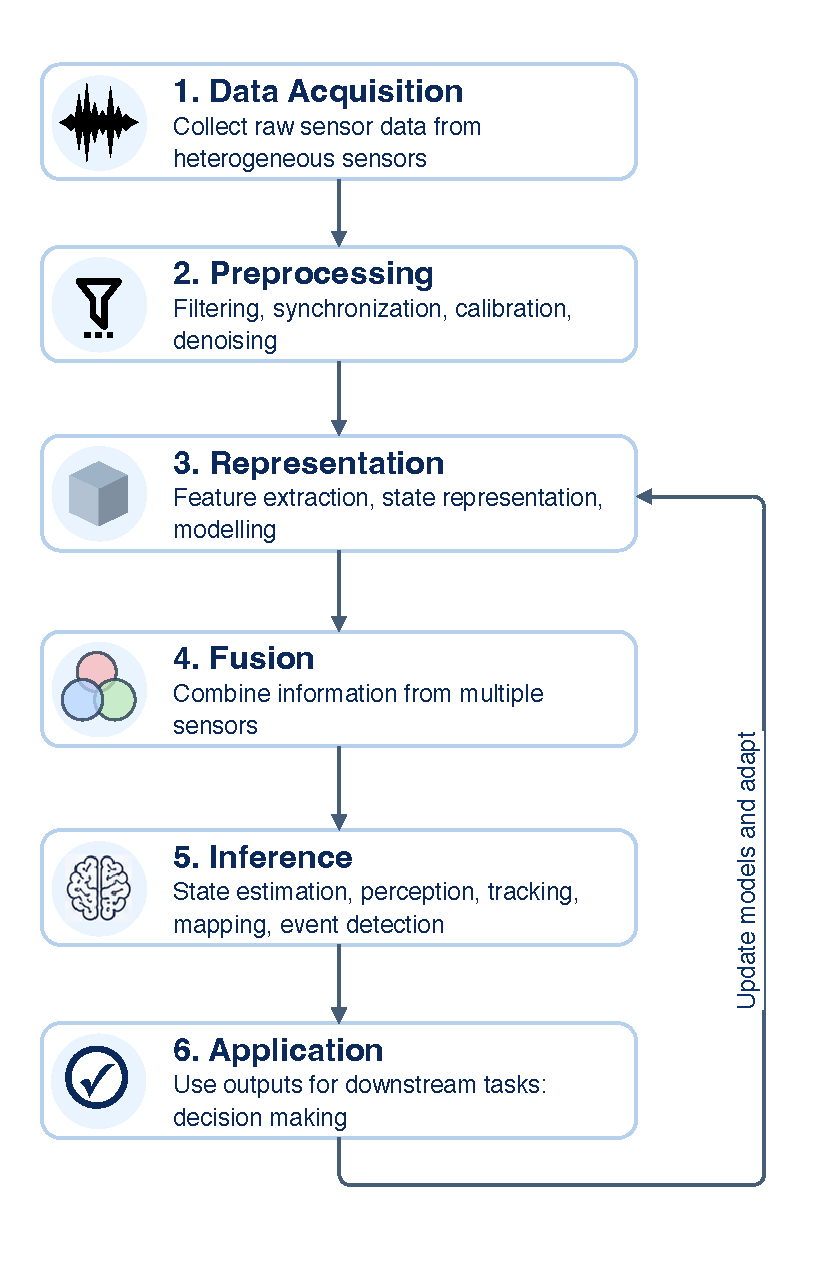
\includegraphics[width=0.85\columnwidth]{figures/fusion_pipeline_v02.pdf}
    \caption{A typical sensor fusion pipeline, from heterogeneous data acquisition to downstream application and feedback-based adaptation.}
    \label{fig:generic-sensor-fusion-pipeline}
\end{figure}

Figure~\ref{fig:generic-sensor-fusion-pipeline} summarises a generic fusion pipeline. The first stage is \emph{data acquisition}, where raw observations are collected from heterogeneous sensors or information sources. These measurements may differ in physical modality, sampling frequency, dimensionality, noise statistics, field of view, latency, and failure modes. The second stage is \emph{preprocessing}, which includes filtering, synchronisation, calibration, denoising, outlier rejection, missing-data handling, and coordinate-frame alignment. This stage is essential because fusion algorithms generally assume that measurements refer to compatible physical quantities, time instants, or spatial frames.

The third stage is \emph{representation}. Depending on the application, sensor measurements may be represented as raw signals, feature vectors, tracks, point clouds, occupancy grids, semantic objects, belief distributions, sets, or learned latent embeddings. The choice of representation strongly affects the level at which fusion is performed. Data-level fusion combines low-level measurements directly; feature-level fusion combines extracted attributes or learned representations; object-level fusion combines detections, tracks, or state estimates; and decision-level fusion combines classifier outputs, alarms, or symbolic decisions. The fourth stage is the actual \emph{fusion} step, in which information from multiple sources is combined using statistical estimation, Bayesian filtering, evidence theory, optimisation, set-membership methods, fuzzy reasoning, machine learning, or hybrid approaches.

The final stages convert fused information into task-relevant knowledge. The \emph{inference} stage estimates states, detects events, tracks objects, maps environments, classifies situations, or predicts future behaviour. The \emph{application} stage then uses these outputs to support downstream tasks such as monitoring, decision-making, planning, control, diagnosis, or human assistance. The feedback arrow in Fig.~\ref{fig:generic-sensor-fusion-pipeline} highlights that practical fusion systems are rarely one-pass pipelines: outputs can be used to update models, adapt sensor weights, refine calibration, select active sensing actions, or reconfigure the system when operating conditions change.

\begin{figure}[!t]
    \centering
    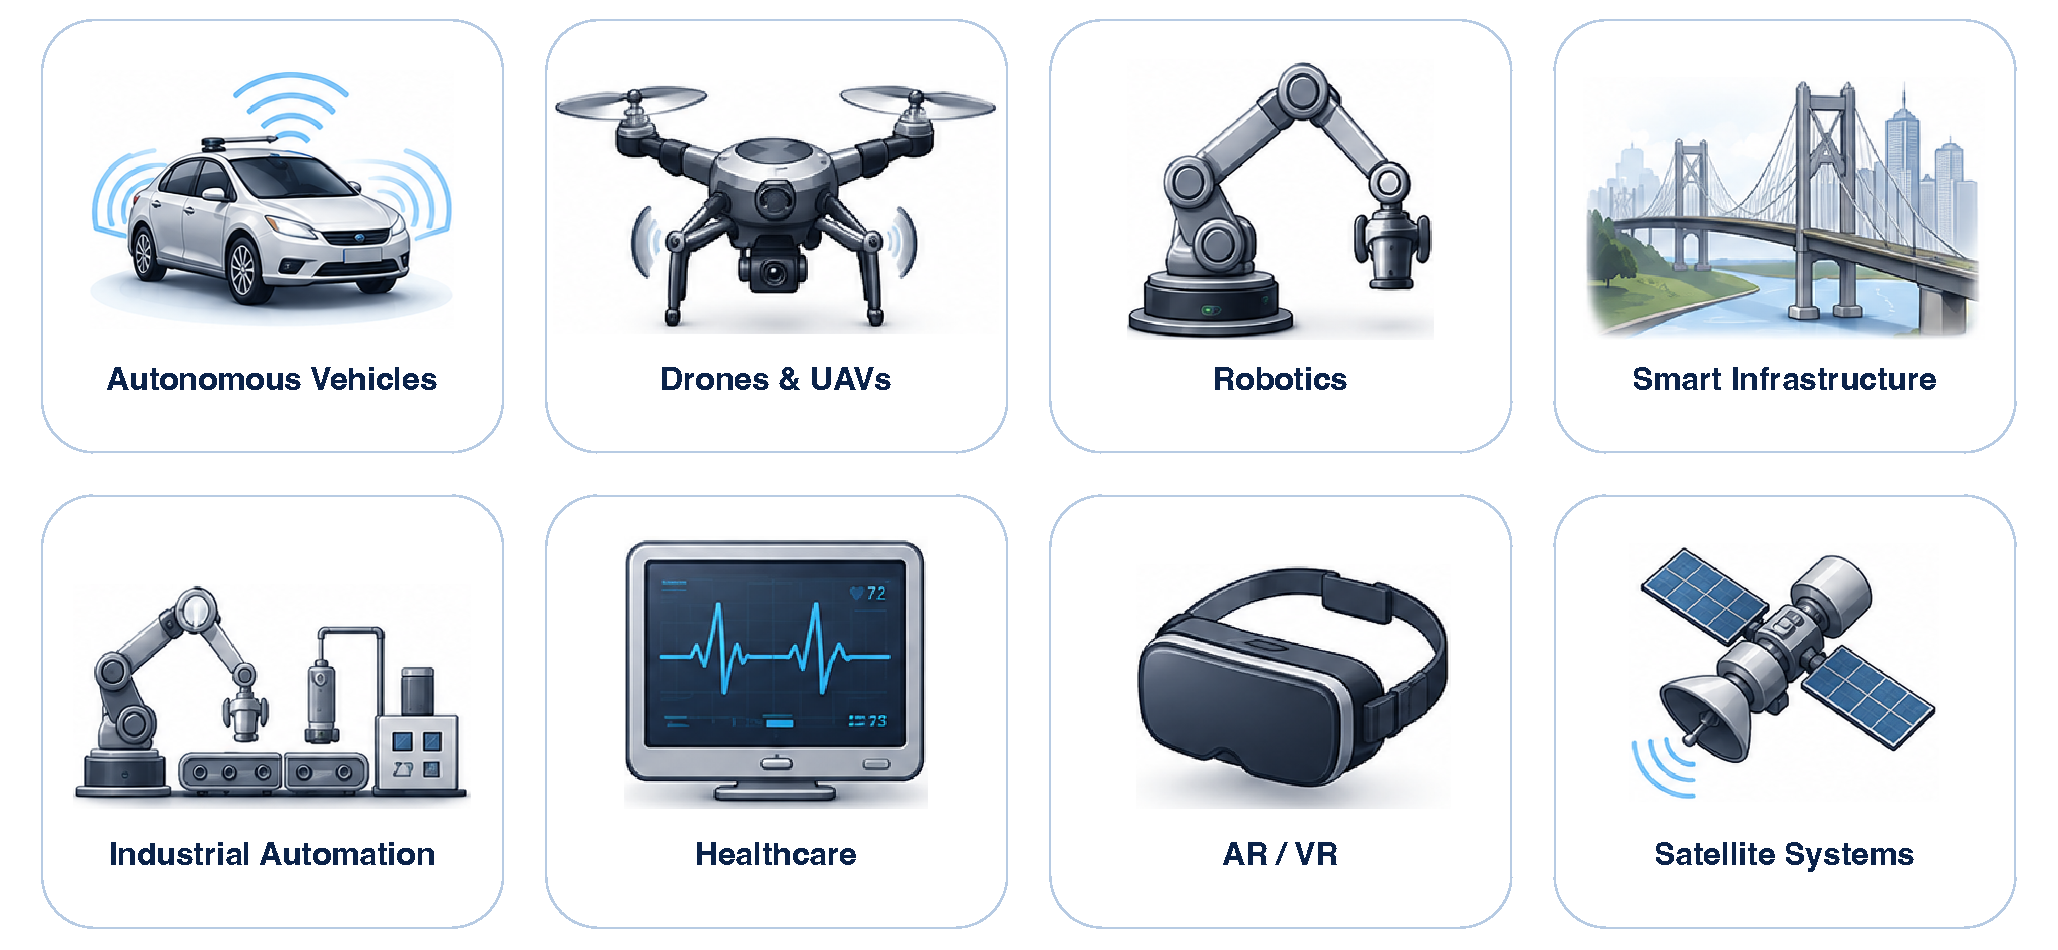
\includegraphics[width=1\columnwidth]{figures/application_areas.pdf}
    \caption{Representative application areas of sensor fusion.}
    \label{fig:application-areas}
\end{figure}

As illustrated in Fig.~\ref{fig:application-areas}, sensor fusion is a cross-domain design pattern rather than a technique restricted to a single field. Autonomous vehicles integrate cameras, radar, LiDAR, inertial sensors, positioning systems, and maps to perceive dynamic road scenes and estimate ego-motion. Drones and unmanned aerial vehicles combine inertial, visual, GNSS, barometric, and range measurements for navigation, stabilisation, obstacle avoidance, and mapping. Robotic systems fuse proprioceptive and exteroceptive sensing to support localisation, manipulation, force control, human--robot interaction, and task planning.

Smart infrastructure combines distributed structural, environmental, traffic, and communication data to monitor bridges, roads, buildings, and energy systems. Industrial automation uses fusion to improve quality control, predictive maintenance, process monitoring, and safe collaboration between humans and machines. Healthcare systems combine physiological, imaging, wearable, and contextual data for diagnosis, monitoring, rehabilitation, and decision support. AR/VR systems fuse cameras, IMUs, depth sensors, eye tracking, and environmental maps to provide robust pose estimation and spatial interaction. Satellite and remote-sensing systems combine optical, radar, thermal, multispectral, and communication data to observe large-scale environmental and human activity.

Although these domains differ substantially, they share a common set of system-level requirements. First, fusion must address \emph{heterogeneity}: the input data may describe appearance, geometry, motion, range, force, acceleration, temperature, physiology, or communication events. Second, fusion must handle \emph{uncertainty}: measurements may be noisy, ambiguous, delayed, intermittent, biased, or contradictory. Third, fusion must satisfy \emph{operational constraints}: many applications require real-time or near-real-time performance on embedded or distributed hardware. Fourth, fusion must support \emph{robustness}: safety-critical systems must continue operating under sensor degradation, environmental changes, communication losses, and out-of-distribution conditions. These requirements explain why the field contains both model-based methods, which provide explicit uncertainty handling and interpretability, and learning-based methods, which provide rich representations for complex multimodal data.

From a design perspective, the main components of a sensor fusion system can therefore be summarised as follows:
\begin{list4a}
    \item \textbf{Sensing sources}: physical sensors, virtual sensors, maps, communication messages, historical data, and model predictions that provide partial information about the system or environment.
    \item \textbf{Temporal and spatial alignment}: synchronisation, interpolation, latency compensation, intrinsic calibration, extrinsic calibration, and coordinate transformations that make heterogeneous data comparable.
    \item \textbf{Representation and abstraction level}: raw measurements, engineered features, learned embeddings, detections, tracks, occupancy maps, semantic maps, probability distributions, bounded sets, or decisions.
    \item \textbf{Uncertainty and reliability modelling}: probabilistic noise models, confidence scores, belief masses, fuzzy memberships, deterministic bounds, sensor-health indicators, and context-dependent reliability weights.
    \item \textbf{Fusion mechanism}: algorithms or architectures that combine information, resolve conflicts, exploit complementarity, handle redundancy, and propagate uncertainty to later stages.
    \item \textbf{Inference and downstream use}: state estimation, perception, tracking, mapping, event detection, prediction, planning, control, monitoring, diagnosis, or decision support.
    \item \textbf{Adaptation and validation}: mechanisms for online model update, failure detection, recalibration, robustness assessment, uncertainty calibration, and verification under representative and rare operating conditions.
\end{list4a}

This system-level view motivates the organisation of the rest of the book. Chapter~\ref{sec:classicalSF} first reviews classical fusion techniques, including probabilistic, statistical, evidence-theoretic, optimisation-based, and set-membership approaches. Chapter~\ref{sec:learning} then examines learning-based and hybrid techniques, where multimodal representations are learned directly from data and combined with model-based estimation or decision-making. Throughout the book, autonomous driving is used as a concrete reference domain, while the underlying principles remain applicable to the broader application areas shown in Fig.~\ref{fig:application-areas}.

\begin{figure}[!t]
    \centering
    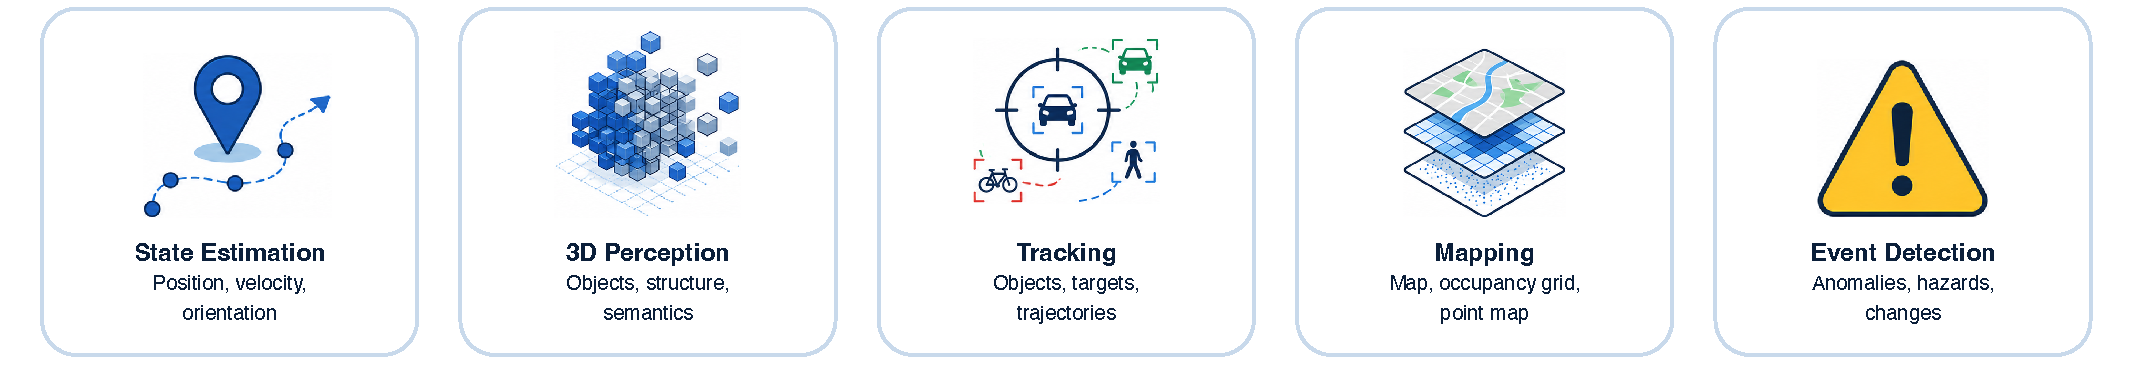
\includegraphics[width=1\columnwidth]{figures/estimates_outputs.pdf}
    \caption{Representative outputs produced by sensor-fusion systems, ranging from state estimates and tracks to maps, decisions, and uncertainty-aware alerts.}
    \label{fig:estimates-outputs}
\end{figure}

Figure~\ref{fig:estimates-outputs} emphasises that the output of a fusion system is not limited to a single point estimate. Depending on the application and abstraction level, fusion may produce filtered state estimates, covariance matrices, bounded state sets, object tracks, occupancy maps, semantic labels, anomaly scores, conflict indicators, reliability weights, or control-relevant decisions. These outputs should be interpreted together with their uncertainty and validity assumptions. For example, a vehicle pose estimate is useful only when accompanied by a covariance, confidence interval, or bounded error envelope; an object detection becomes more valuable when associated with a track identity and existence confidence; and a decision-level alert is safer when it exposes whether sensors agree, disagree, or are degraded. This motivates the transition from system components to the classical mathematical tools reviewed in the next section.

% ============================================
%
%
\chapter{Classical Sensor Fusion Techniques}
\label{sec:classicalSF}
%
%
% ============================================

% ============================================
\section{Mathematical introduction to sensor fusion}
% ============================================

Sensor fusion concerns the estimation of an unknown physical quantity from multiple measurements that may differ in modality, dimension, accuracy, sampling rate, and uncertainty. The quantity to be estimated may be a static parameter, such as the location of a stationary source, or a time-varying state, such as the position, velocity, and orientation of a moving vehicle. Table~\ref{tab:notation} collects the notation used throughout the book and records where symbols are reused with different meanings across the method families reviewed here.
\begin{table}[!t]
    \centering
    \small
    \caption{\textcolor{olive}{[To be updated at the end]} Principal notation. Symbols are reused across method families where the literatures conflict; the scope column states where each reading applies.}
    \label{tab:notation}
    \begin{tabular}{p{0.13\linewidth} p{0.44\linewidth} p{0.28\linewidth}}
        \hline
        \textbf{Symbol} & \textbf{Meaning} & \textbf{Scope} \\
        \hline
        $\mathbf{x}$, $\widehat{\mathbf{x}}$ & state, estimate & throughout \\
        $\mathbf{y}$, $\mathbf{r}$ & measurement, measurement noise & throughout \\
        $\mathbf{g}(\cdot)$, $\mathbf{G}$ & measurement function, measurement matrix & throughout \\
        $\mathbf{f}(\cdot)$, $\mathbf{q}$ & process model, process noise & dynamic models \\
        $\mathbf{R}$, $\mathbf{Q}$, $\mathbf{P}$ & measurement, process, state covariance & probabilistic fusion \\
        $\mathbf{\Lambda}$ & information matrix, $\mathbf{P}^{-1}$ & probabilistic fusion \\
        $\boldsymbol{\nu}$, $\mathbf{S}$, $\mathbf{K}$ & innovation, its covariance, gain & filtering \\
        $\mathbf{m}$ & prior mean & regularised least squares \\
        $p$, $H$, $\gamma$ & zonotope centre, generators, strip gain & set-membership \\
        $\Omega$, $m(\cdot)$, $K$ & frame of discernment, belief mass, conflict & evidence theory \\
        $w$, $q$, $\mu$ & fusion weight, quality indicator, membership & reliability-aware fusion \\
        $\mathcal{G}$, $\mathcal{N}_i$ & communication graph, neighbour set & multi-agent fusion \\
        \hline
    \end{tabular}
\end{table}





% ============================================
\subsection{Sensor fusion as an inverse problem}
% ============================================
Let $\mathbf{x}\in\mathbb{R}^{d_x}$ denote the unknown state or parameter vector. The $n$-th sensor measurement is modelled as
\begin{align}
\mathbf{y}_n=\mathbf{g}_n(\mathbf{x})+\mathbf{r}_n, \qquad n=1,\ldots,N,
\end{align}
where $\mathbf{y}_n\in\mathbb{R}^{d_n}$ is the observed measurement, $\mathbf{g}_n:\mathbb{R}^{d_x}\rightarrow\mathbb{R}^{d_n}$ is the measurement or observation function of sensor $n$, and $\mathbf{r}_n\in\mathbb{R}^{d_n}$ represents measurement noise and modelling error.

The sensor-fusion problem is therefore an inverse problem: the forward models $\mathbf{g}_n(\cdot)$ describe how a hypothetical state produces measurements, while fusion attempts to infer the state that most plausibly explains the measurements actually observed. 

Different sensors need not measure the state directly. For example, a GNSS receiver may provide a noisy position measurement,
\begin{align*}
\mathbf{y}_{\mathrm{GNSS}}=\mathbf{p}+\mathbf{r}_{\mathrm{GNSS}},
\end{align*}
whereas a range sensor located at $\mathbf{s}_n$ may provide
\begin{align*}
y_n=\left\|\mathbf{p}-\mathbf{s}_n\right\|_2+r_n.
\end{align*}
A camera may instead provide a perspective projection,
\begin{align*}
\Pi\left(\boldsymbol{\mathcal{R}}\,\mathbf{p}+\mathbf{t}\right) +\mathbf{r}_n,
\end{align*}
where $\Pi(\cdot)$ is a nonlinear projection operator and $\boldsymbol{\mathcal{R}}$ is a rotation matrix. Sensor fusion places all such measurements within a common estimation framework despite their different physical interpretations.

% ============================================
\subsection{Measurement uncertainty}
% ============================================
Measurements are not exact. Their uncertainty can arise from thermal noise, quantisation, imperfect calibration, environmental interference, finite resolution, unmodelled dynamics, or errors in the assumed sensor model.

A standard starting assumption is that the measurement error has zero mean, $\mathbb{E}[\mathbf{r}_n]=\mathbf{0}_{d_n}$, and covariance $\mathbf{R}_n\in\mathbb{R}^{d_n\times d_n}$. The covariance matrix $\mathbf{R}_n$ describes both the magnitude and the directional structure of the uncertainty. For a scalar measurement, $y_n=g_n(\mathbf{x})+r_n$, the covariance reduces to the variance $\operatorname{var}(r_n)=\sigma_n^2$. A larger $\sigma_n^2$ means that the measurement is less precise. For a vector measurement $\mathbf{y}\triangleq \begin{bmatrix} y_{1} & y_{2} & \cdots & y_{d_n} \end{bmatrix}^T \in \mathbb{R}^{d_n}$,
\begin{align*}
\mathbf{R}=
\begin{bmatrix}
\operatorname{var}(r_{1}) & \operatorname{cov}(r_{1},r_{2}) & \cdots & \operatorname{cov}(r_{1},r_{d_n})\\
\operatorname{cov}(r_{2},r_{1}) & \operatorname{var}(r_{2}) & \cdots & \operatorname{cov}(r_{2},r_{d_n}) \\
\vdots & \vdots & \ddots & \vdots\\
\operatorname{cov}(r_{d_n},r_{1})  & \operatorname{cov}(r_{d_n},r_{2}) & \cdots & \operatorname{var}(r_{d_n}) \\
\end{bmatrix},
\end{align*}
the diagonal entries represent component-wise variances, while the off-diagonal entries represent correlations between measurement components. When the off-diagonal terms are non-zero, the measurement components are correlated, and the uncertainty region is tilted with respect to the coordinate axes. An eigenvalue decomposition removes the tilt by rotating into the axes along which the errors are uncorrelated. For a two-dimensional position measurement
the correlated uncertainty region then becomes an ellipse,
%Geometrically, this means the shape of the uncertainty is tilted relative to our standard axes. To simplify this shape, we use eigenvalue decomposition. This tool rotates our coordinate system to align perfectly with the orientation of the uncertainty. In this new coordinate system, the correlation disappears, and the errors become completely independent. For a two-dimensional position measurement, this transformation maps the correlated uncertainty region into an uncertainty ellipse defined by:
\begin{align*}
\mathbf{R}=\mathbf{U}\left[\begin{matrix}\lambda _{1}&0\\ 0&\lambda _{2}\end{matrix}\right]\mathbf{U}^{\mathsf{T}} \;.
\end{align*}
In this decoupled form, the eigenvectors in $\mathbf{U}$ serve as a rotation matrix that determines the principal axes (directions) of the uncertainty ellipse. Meanwhile, the eigenvalues $\lambda _{1}$ and $\lambda _{2}$ represent the decoupled variances, directly dictating the lengths (magnitudes) of the ellipse's semi-axes along those new directions.

% ============================================
\subsection{Independent and correlated measurement errors}
% ============================================
A common simplifying assumption is that the errors of different measurements are mutually independent. Under this assumption, measurements may have different covariance matrices, but their errors do not share common random components. Independence is reasonable when measurements arise from physically separate noise processes. It may be violated, however, when sensors share calibration parameters, environmental disturbances, timing errors, communication links, or preprocessing algorithms. For example, two position estimates derived from the same camera images generally have correlated errors. Likewise, repeated measurements from the same biased sensor may be strongly correlated even when their high-frequency noise samples are independent. The distinction is important because treating correlated measurements as independent effectively counts shared information more than once, causing an estimator to become overconfident\footnote{The intuition is simple: if two sensors share a common disturbance, calibration error, map error, timing error, or modelling error, then their mistakes tend to point in the same direction. Seeing both sensors agree does not mean the estimate is twice as reliable. They may agree because they are affected by the same hidden error.}.

Mathematically, the absence of correlation between two different measurement errors can be described through their cross-covariance. For measurements indexed by $m$ and $n$, this cross-covariance is defined as
\begin{equation}
\operatorname{cov}(\mathbf{r}_m,\mathbf{r}_n) = \mathbb{E}\left[\left(\mathbf{r}_m-\mathbb{E}[\mathbf{r}_m]\right)\left(\mathbf{r}_n-\mathbb{E}[\mathbf{r}_n]\right)^{\mathsf T}\right].
\end{equation}
Thus, the assumption that different measurement errors are uncorrelated is written as
\begin{equation}
\operatorname{cov}(\mathbf{r}_m,\mathbf{r}_n) = \mathbf{0}, \quad m\neq n.
\end{equation}
It is useful to distinguish between being uncorrelated and being independent. Independence implies zero cross-covariance, provided the covariance exists. The reverse is not true in general. However, when the errors are jointly Gaussian, zero cross-covariance is sufficient to imply independence. This is one reason why Gaussian models are especially convenient in sensor fusion.

% ============================================
\subsection{Stacked measurement model}
% ============================================
Sensor fusion becomes particularly transparent when all measurements are written in a common stacked form. Starting from the individual measurement models
\begin{equation}
\mathbf{y}_n
=
\mathbf{g}_n(\mathbf{x})
+
\mathbf{r}_n,
\qquad n=1,\ldots,N,
\end{equation}
we define the stacked measurement vector as
\begin{equation}
\underbrace{\begin{bmatrix}
\mathbf{y}_1\\
\mathbf{y}_2\\
\vdots\\
\mathbf{y}_N
\end{bmatrix}}_{\triangleq \mathbf{y}} = 
\underbrace{\begin{bmatrix}
\mathbf{g}_1(\mathbf{x})\\
\mathbf{g}_2(\mathbf{x})\\
\vdots\\
\mathbf{g}_N(\mathbf{x})
\end{bmatrix}}_{\triangleq \mathbf{g}(\mathbf{x})} + 
\underbrace{\begin{bmatrix}
\mathbf{r}_1\\
\mathbf{r}_2\\
\vdots\\
\mathbf{r}_N
\end{bmatrix}.}_{\triangleq \mathbf{r}}
\end{equation}
This compact representation is important because it allows heterogeneous measurements to be handled in a unified way. The entries of $\mathbf{y}$ may include positions, velocities, accelerations, ranges, bearings, pixel coordinates, signal strengths, or other sensor outputs. The role of $\mathbf{g}(\mathbf{x})$ is to predict, for a given candidate state $\mathbf{x}$, what each sensor should observe.

The covariance of the stacked noise vector is
\begin{equation}
\mathbf{R}
\triangleq
\operatorname{cov}(\mathbf{r}) = \mathbb{E} \left[ \left( \mathbf{r}-\mathbb{E}[\mathbf{r}] \right) \left( \mathbf{r}-\mathbb{E}[\mathbf{r}] \right)^{\mathsf T} \right].
\end{equation}
If the measurement errors are mutually uncorrelated, then the covariance matrix has the block-diagonal structure
\begin{equation}
\mathbf{R}=
\begin{bmatrix}
\mathbf{R}_1 & \mathbf{0} & \cdots & \mathbf{0}\\
\mathbf{0} & \mathbf{R}_2 & \cdots & \mathbf{0}\\
\vdots & \vdots & \ddots & \vdots\\
\mathbf{0} & \mathbf{0} & \cdots & \mathbf{R}_N
\end{bmatrix}.
\end{equation}
If the measurement errors are correlated, the covariance matrix instead contains nonzero off-diagonal blocks:
\begin{equation}
\mathbf{R}
=
\begin{bmatrix}
\mathbf{R}_{11} & \mathbf{R}_{12} & \cdots & \mathbf{R}_{1N}\\
\mathbf{R}_{21} & \mathbf{R}_{22} & \cdots & \mathbf{R}_{2N}\\
\vdots & \vdots & \ddots & \vdots\\
\mathbf{R}_{N1} & \mathbf{R}_{N2} & \cdots & \mathbf{R}_{NN}
\end{bmatrix}.
\end{equation}
The diagonal block $\mathbf{R}_{nn}$ describes the uncertainty of the $n$th measurement, while the off-diagonal block $\mathbf{R}_{mn}$ is
\begin{equation}
\mathbf{R}_{mn} = \operatorname{cov}(\mathbf{r}_m,\mathbf{r}_n).
\end{equation}
These off-diagonal terms should not be ignored when sensors share common sources of uncertainty. If they are ignored, the estimator may behave as if more independent information is available than there really is.

% ============================================
\subsection{Gaussian measurement model}
% ============================================
A common and analytically convenient assumption is that the stacked measurement noise is Gaussian, i.e., $\mathbf{r} \sim \mathcal{N} \left( \mathbf{0}, \mathbf{R} \right)$. Since the measurement model is $\mathbf{y}=\mathbf{g}(\mathbf{x})+\mathbf{r}$, the conditional distribution of the measurements given the state is $\mathbf{y}\mid\mathbf{x} \sim \mathcal{N} \left( \mathbf{g}(\mathbf{x}), \mathbf{R} \right)$. 
The corresponding likelihood is
\begin{align}
\label{eq:Gaussianlikelihood}
p(\mathbf{y}\mid\mathbf{x}) =& \frac{1} {(2\pi)^{d_y/2}|\mathbf{R}|^{1/2}}\times  \\ 
&\exp \left( - \frac{1}{2} \left( \mathbf{y}-\mathbf{g}(\mathbf{x})\right)^{\mathsf T}\mathbf{R}^{-1}\left(\mathbf{y}-\mathbf{g}(\mathbf{x})\right)\right), \nonumber
\end{align}
where $d_y$ is the dimension of the stacked measurement vector. This expression shows that the plausibility of a state is not determined by the residual alone, but by the residual relative to the uncertainty. A residual of a given numerical size may be significant for a precise sensor and insignificant for a noisy sensor.

% ============================================
\subsection{Residuals, least squares, and optimality criteria}
% ============================================
For a candidate state $\mathbf{x}$, the residual is defined as
\begin{align}
\mathbf{e}(\mathbf{x}) \triangleq \mathbf{y} - \mathbf{g}(\mathbf{x}).
\end{align}
The residual measures the discrepancy between the actual measurements and the measurements predicted by the model. Sensor fusion can therefore be formulated as the problem of finding the state that makes the residual small in an appropriate sense.

An estimator is obtained by minimising a cost function:
\begin{align}
\widehat{\mathbf{x}} = \operatorname*{arg\,min}_{\mathbf{x}} J(\mathbf{x}).
\end{align}
Different choices of $J(\mathbf{x})$ correspond to different assumptions about the measurement errors and different notions of optimality. Least-squares methods use a quadratic cost. For scalar measurements, the ordinary least-squares cost is
\begin{align}
J_{\mathrm{LS}}(\mathbf{x}) = \sum_{n=1}^{N}\left(y_n-g_n(\mathbf{x})\right)^2.
\end{align}
For vector-valued measurements, this becomes
\begin{align}
J_{\mathrm{LS}}(\mathbf{x}) &=\sum_{n=1}^{N}\left(\mathbf{y}_n-\mathbf{g}_n(\mathbf{x})\right)^{\mathsf T}\left(\mathbf{y}_n-\mathbf{g}_n(\mathbf{x})\right) \nonumber \\
&= \left( \mathbf{y} - \mathbf{g}(\mathbf{x}) \right)^{\mathsf T}\left(\mathbf{y}-\mathbf{g}(\mathbf{x})\right) \nonumber \\
& = \left\|\mathbf{y} - \mathbf{g}(\mathbf{x}) \right\|_2^2 . % [July 2026 pass] removed stray {\color{blue}.} left over from a first-round edit
\end{align}
The corresponding ordinary least-squares estimate is
\begin{align}
\widehat{\mathbf{x}}_{\mathrm{LS}} = \operatorname*{arg\,min}_{\mathbf{x}} \left\| \mathbf{y} - \mathbf{g}(\mathbf{x}) \right\|_2^2.
\end{align}
Ordinary least squares is simple and often effective, but it treats all residual components equally. This can be inappropriate in sensor fusion because measurements may have different units, different noise levels, and different reliability.

Consider first the linear case, in which every measurement function is linear, so that the stacked model of the previous subsection reduces to
\begin{align}
\mathbf{y}=\mathbf{G}\mathbf{x}+\mathbf{r},
\label{eq:linear-measurement-model}
\end{align}
where $\mathbf{G}\in\mathbb{R}^{d_y\times d_x}$ in~\eqref{eq:linear-measurement-model} stacks the individual measurement matrices $\mathbf{G}_n$ vertically. Each row of $\mathbf{G}$ states how one scalar measurement responds to the unknown state.
For this linear model, the ordinary least-squares cost is
\begin{align}
J_{\mathrm{LS}}(\mathbf{x}) = \left( \mathbf{y} - \mathbf{G}\mathbf{x} \right)^{\mathsf T} \left( \mathbf{y} - \mathbf{G}\mathbf{x} \right).
\end{align}
The gradient with respect to $\mathbf{x}$ is
\begin{align}
\nabla_{\mathbf{x}} J_{\mathrm{LS}}(\mathbf{x}) = -2 \mathbf{G}^{\mathsf T} \mathbf{y} + 2 \mathbf{G}^{\mathsf T} \mathbf{G} \mathbf{x}.
\end{align}
At the minimum, the gradient is zero. Hence,
\begin{align}
\mathbf{G}^{\mathsf T} \mathbf{G} \widehat{\mathbf{x}}_{\mathrm{LS}} = \mathbf{G}^{\mathsf T} \mathbf{y}.
\end{align}
If $\mathbf{G}^{\mathsf T}\mathbf{G}$ is invertible, the solution is
\begin{align}
\widehat{\mathbf{x}}_{\mathrm{LS}} = \left( \mathbf{G}^{\mathsf T} \mathbf{G} \right)^{-1} \mathbf{G}^{\mathsf T} \mathbf{y}.
\end{align}
The invertibility of $\mathbf{G}^{\mathsf T}\mathbf{G}$ requires the columns of $\mathbf{G}$ to be linearly independent. In sensor-fusion terms, this means that the available measurements must contain enough independent information to identify all components of $\mathbf{x}$. If this condition fails, the estimate may be non-unique or highly sensitive to noise.
Substituting the model $\mathbf{y}=\mathbf{G}\mathbf{x}+\mathbf{r}$ into the estimator gives
\begin{align}
\widehat{\mathbf{x}}_{\mathrm{LS}} = \mathbf{x} + \left( \mathbf{G}^{\mathsf T} \mathbf{G} \right)^{-1} \mathbf{G}^{\mathsf T} \mathbf{r}.
\end{align}
Assuming the noise is zero mean, taking expectations yields
\begin{align}
\mathbb{E} \left[ \widehat{\mathbf{x}}_{\mathrm{LS}} \right] = \mathbf{x},
\end{align}
so the estimator is unbiased when the model is correct and the noise is zero mean. Its covariance is
\begin{align}
\operatorname{cov} \left( \widehat{\mathbf{x}}_{\mathrm{LS}} \right) =
\left(
\mathbf{G}^{\mathsf T}
\mathbf{G}
\right)^{-1}
\mathbf{G}^{\mathsf T}
\mathbf{R}
\mathbf{G}
\left(
\mathbf{G}^{\mathsf T}
\mathbf{G}
\right)^{-1}.
\end{align}
If the noise covariance is $\mathbf{R}=\sigma^2\mathbf{I}$, this simplifies to
\begin{align}
\operatorname{cov} \left(\widehat{\mathbf{x}}_{\mathrm{LS}} \right) = \sigma^2\left( \mathbf{G}^{\mathsf T} \mathbf{G} \right)^{-1}.
\end{align}
This expression shows that estimation uncertainty depends not only on the sensor noise level, but also on the geometry and conditioning of the measurement matrix.

\subsection{Weighted least squares and the information matrix}

Weighted least squares (WLS) incorporates measurement uncertainty directly into the cost function. Instead of penalising all residuals equally, it weights the residual according to the inverse covariance matrix:
\begin{align}
J_{\mathrm{WLS}}(\mathbf{x}) = \left( \mathbf{y} - \mathbf{G}\mathbf{x} \right)^{\mathsf T} \mathbf{R}^{-1} \left( \mathbf{y} - \mathbf{G}\mathbf{x} \right).
\end{align}
This quantity is the squared Mahalanobis norm of the residual:
\begin{align}
J_{\mathrm{WLS}}(\mathbf{x}) = \left\| \mathbf{y} - \mathbf{G}\mathbf{x} \right\|_{\mathbf{R}^{-1}}^2.
\end{align}
The interpretation is as follows: residuals are measured relative to their uncertainty. A residual from a precise sensor is penalised more strongly than the same residual from a noisy sensor. 
Proceeding exactly as in the unweighted case, the gradient
\begin{align}
\nabla_{\mathbf{x}}
J_{\mathrm{WLS}}(\mathbf{x}) = -2 \mathbf{G}^{\mathsf T} \mathbf{R}^{-1} \mathbf{y} + 2 \mathbf{G}^{\mathsf T} \mathbf{R}^{-1} \mathbf{G} \mathbf{x}
\end{align}
vanishes where $$\mathbf{G}^{\mathsf T}\mathbf{R}^{-1}\mathbf{G}\,\widehat{\mathbf{x}}_{\mathrm{WLS}}=\mathbf{G}^{\mathsf T}\mathbf{R}^{-1}\mathbf{y},$$ so that whenever $\mathbf{G}^{\mathsf T}\mathbf{R}^{-1}\mathbf{G}$ is invertible
%The gradient of the WLS cost is
%\begin{align}
%\nabla_{\mathbf{x}}
%J_{\mathrm{WLS}}(\mathbf{x}) = -2 \mathbf{G}^{\mathsf T} \mathbf{R}^{-1} \mathbf{y} %+ 2 \mathbf{G}^{\mathsf T} \mathbf{R}^{-1} \mathbf{G} \mathbf{x}.
%\end{align}
%Setting the gradient to zero gives:
%\begin{align}
%\mathbf{G}^{\mathsf T}
%\mathbf{R}^{-1}
%\mathbf{G}
%\widehat{\mathbf{x}}_{\mathrm{WLS}}
%=
%\mathbf{G}^{\mathsf T}
%\mathbf{R}^{-1}
%\mathbf{y}.
%\end{align}
%If $\mathbf{G}^{\mathsf T}\mathbf{R}^{-1}\mathbf{G}$ is invertible, then
\begin{align}
\widehat{\mathbf{x}}_{\mathrm{WLS}}
=
\left(
\mathbf{G}^{\mathsf T}
\mathbf{R}^{-1}
\mathbf{G}
\right)^{-1}
\mathbf{G}^{\mathsf T}
\mathbf{R}^{-1}
\mathbf{y}.
\end{align}
Substituting $\mathbf{y}=\mathbf{G}\mathbf{x}+\mathbf{r}$ gives
\begin{align}
\widehat{\mathbf{x}}_{\mathrm{WLS}}
=
\mathbf{x}
+
\left(
\mathbf{G}^{\mathsf T}
\mathbf{R}^{-1}
\mathbf{G}
\right)^{-1}
\mathbf{G}^{\mathsf T}
\mathbf{R}^{-1}
\mathbf{r}.
\end{align}
Therefore, for $\mathbb{E}
\left[\mathbf{r}\right]
=\mathbf{0}$, the estimator is unbiased, i.e., $\mathbb{E} \left[\widehat{\mathbf{x}}_{\mathrm{WLS}} \right] = \mathbf{x}$. The covariance of the WLS estimator is
\begin{align}
\operatorname{cov}
\left(
\widehat{\mathbf{x}}_{\mathrm{WLS}}
\right)
=
\left(
\mathbf{G}^{\mathsf T}
\mathbf{R}^{-1}
\mathbf{G}
\right)^{-1}.
\end{align}
The matrix
\begin{align}
\mathbf{\Lambda}
=
\mathbf{G}^{\mathsf T}
\mathbf{R}^{-1}
\mathbf{G}
\end{align}
is often called the \emph{information matrix}. It measures how much information the measurements provide about the unknown state. The covariance is the inverse of this information matrix, i.e., $\operatorname{cov} \left( \widehat{\mathbf{x}}_{\mathrm{WLS}} \right) = \mathbf{\Lambda}^{-1}$.

Weighted least squares has a direct maximum-likelihood interpretation. Assume that $\mathbf{r}
\sim
\mathcal{N}
\left(
\mathbf{0},
\mathbf{R}
\right)$. Then, $\mathbf{y}\mid\mathbf{x}
\sim
\mathcal{N}
\left(
\mathbf{g}(\mathbf{x}),
\mathbf{R}
\right)$.
The maximum-likelihood estimate is defined as
\begin{equation}
\widehat{\mathbf{x}}_{\mathrm{ML}}
=
\operatorname*{arg\,max}_{\mathbf{x}}
p(\mathbf{y}\mid\mathbf{x}).
\end{equation}
Equivalently, it minimises the negative log-likelihood. Ignoring terms that do not depend on $\mathbf{x}$, from~\eqref{eq:Gaussianlikelihood} we obtain
\begin{align*}
-\log p(\mathbf{y}\mid\mathbf{x}) =
\frac{1}{2}
\left(\mathbf{y} - \mathbf{g}(\mathbf{x}) \right)^{\mathsf T}
\mathbf{R}^{-1}
\left(
\mathbf{y}
-
\mathbf{g}(\mathbf{x})
\right)
+
C.
\end{align*}
Therefore,
\begin{equation}
\widehat{\mathbf{x}}_{\mathrm{ML}}
=
\operatorname*{arg\,min}_{\mathbf{x}}
\left(
\mathbf{y}
-
\mathbf{g}(\mathbf{x})
\right)^{\mathsf T}
\mathbf{R}^{-1}
\left(
\mathbf{y}
-
\mathbf{g}(\mathbf{x})
\right).
\end{equation}
Thus, under additive Gaussian measurement noise, $\widehat{\mathbf{x}}_{\mathrm{ML}} = \widehat{\mathbf{x}}_{\mathrm{WLS}}$. This result explains why least-squares methods are so widely used in sensor fusion. They can be derived either from an optimisation viewpoint, by minimising weighted residuals, or from a probabilistic viewpoint, by maximising a Gaussian likelihood.

\subsection{Prior information: regularised least squares and the MAP estimate}
In some problems, measurements alone are insufficient to estimate $\mathbf{x}$ reliably. This may occur when the number of measurements is small, when the measurement geometry is poor, when the inverse problem is ill-conditioned, or when some components of the state are weakly observable. Regularised least squares addresses this by incorporating prior information. Let $\mathbf{m}$ denote a prior estimate of $\mathbf{x}$, and let $\mathbf{P}$ denote the covariance associated with this prior. A small $\mathbf{P}$ means that the prior is trusted strongly; a large $\mathbf{P}$ means that the prior is weak. The regularised least-squares cost is
\begin{align}
J_{\mathrm{ReLS}}(\mathbf{x})
=&
\left(
\mathbf{y}
-
\mathbf{G}\mathbf{x}
\right)^{\mathsf T}
\mathbf{R}^{-1}
\left(
\mathbf{y}
-
\mathbf{G}\mathbf{x}
\right) \nonumber \\
&+
\left(
\mathbf{x}
-
\mathbf{m}
\right)^{\mathsf T}
\mathbf{P}^{-1}
\left(
\mathbf{x}
-
\mathbf{m}
\right).
\end{align}
The first term measures consistency with the sensor data. The second term measures consistency with the prior. Differentiating and setting the gradient to zero gives
\begin{equation}
\left(
\mathbf{G}^{\mathsf T}
\mathbf{R}^{-1}
\mathbf{G}
+
\mathbf{P}^{-1}
\right)
\widehat{\mathbf{x}}_{\mathrm{ReLS}}
=
\mathbf{G}^{\mathsf T}
\mathbf{R}^{-1}
\mathbf{y}
+
\mathbf{P}^{-1}
\mathbf{m}.
\end{equation}
Therefore,
\begin{equation}
\widehat{\mathbf{x}}_{\mathrm{ReLS}}
=
\left(
\mathbf{G}^{\mathsf T}
\mathbf{R}^{-1}
\mathbf{G}
+
\mathbf{P}^{-1}
\right)^{-1}
\left(
\mathbf{G}^{\mathsf T}
\mathbf{R}^{-1}
\mathbf{y}
+
\mathbf{P}^{-1}
\mathbf{m}
\right).
\end{equation}
This estimator combines measurement information and prior information. The measurement information matrix is
\begin{equation}
\mathbf{\Lambda}_{\mathrm{meas}}
=
\mathbf{G}^{\mathsf T}
\mathbf{R}^{-1}
\mathbf{G},
\end{equation}
and the prior information matrix is
\begin{equation}
\mathbf{\Lambda}_{\mathrm{prior}}
=
\mathbf{P}^{-1}.
\end{equation}
The posterior information matrix is their sum:
\begin{equation}
\mathbf{\Lambda}_{\mathrm{post}}
=
\mathbf{G}^{\mathsf T}
\mathbf{R}^{-1}
\mathbf{G}
+
\mathbf{P}^{-1}.
\end{equation}
Hence, the posterior covariance is
\begin{equation}
\mathbf{P}^{+}
=
\left(
\mathbf{G}^{\mathsf T}
\mathbf{R}^{-1}
\mathbf{G}
+
\mathbf{P}^{-1}
\right)^{-1}.
\end{equation}
Unlike ordinary LS and WLS, the regularised estimator is generally pulled toward the prior mean $\mathbf{m}$. From a frequentist perspective, this may introduce bias. From a Bayesian perspective, it reflects the deliberate use of prior knowledge.

Regularised least squares has a natural Bayesian interpretation. Suppose that the prior distribution of the unknown state is Gaussian, i.e., $\mathbf{x}
\sim
\mathcal{N}
\left(
\mathbf{m},
\mathbf{P}
\right)$. Suppose also that the measurement model is linear and Gaussian:
\begin{equation}
\mathbf{y}\mid\mathbf{x}
\sim
\mathcal{N}
\left(
\mathbf{G}\mathbf{x},
\mathbf{R}
\right).
\end{equation}
Bayes' rule gives
\begin{equation}
p(\mathbf{x}\mid\mathbf{y})
=
\frac{
p(\mathbf{y}\mid\mathbf{x})p(\mathbf{x})
}{
p(\mathbf{y})
}.
\end{equation}
The maximum a posteriori estimate is
\begin{equation}
\widehat{\mathbf{x}}_{\mathrm{MAP}}
=
\operatorname*{arg\,max}_{\mathbf{x}}
p(\mathbf{x}\mid\mathbf{y}).
\end{equation}
Equivalently, it minimises the negative log-posterior. Ignoring constants independent of $\mathbf{x}$, this gives
\begin{align}
\widehat{\mathbf{x}}_{\mathrm{MAP}}
=
\operatorname*{arg\,min}_{\mathbf{x}}
\bigg[
&\left(
\mathbf{y}
-
\mathbf{G}\mathbf{x}
\right)^{\mathsf T}
\mathbf{R}^{-1}
\left(
\mathbf{y}
-
\mathbf{G}\mathbf{x}
\right) \nonumber \\
&+
\left(
\mathbf{x}
-
\mathbf{m}
\right)^{\mathsf T}
\mathbf{P}^{-1}
\left(
\mathbf{x}
-
\mathbf{m}
\right)
\bigg].
\end{align}
Therefore,
\begin{equation}
\widehat{\mathbf{x}}_{\mathrm{MAP}}
=
\widehat{\mathbf{x}}_{\mathrm{ReLS}}.
\end{equation}
This result is important because it unifies deterministic optimisation and probabilistic inference. The same estimator can be interpreted either as the minimiser of a regularised cost or as the most probable state after combining a Gaussian prior with Gaussian measurements.

% ============================================
\subsection{Sequential least squares}
% ============================================
\label{subsubsec:sequential_least_squares}

In the batch formulation, all measurements are collected first and the estimate is computed by solving one weighted least-squares problem. This is suitable when the complete data set is available in advance. In many sensor-fusion applications, however, measurements arrive sequentially. For example, a mobile robot may receive one range measurement, then a camera feature, then an inertial reading, and so on. Recomputing the full batch solution after every new measurement is possible, but it is often computationally inefficient and unnecessary.

Sequential least squares provides an equivalent recursive way of updating the estimate. Instead of storing and reprocessing all previous measurements, it summarises the information contained in the past measurements by the current estimate and its covariance. When a new measurement arrives, the estimate is corrected using only the new measurement, the previous estimate, and the previous covariance.

Suppose that after processing measurements up to step $n-1$, the available estimate is $\widehat{\mathbf{x}}_{n-1}$, and its uncertainty is described by the covariance matrix $\mathbf{P}_{n-1}$. The covariance $\mathbf{P}_{n-1}$ quantifies how uncertain the estimator is about the current value of the unknown static parameter $\mathbf{x}$. A new measurement arrives according to the linear model
\begin{align*}
\mathbf{y}_n
=
\mathbf{G}_n\mathbf{x}
+
\mathbf{r}_n,
\quad
\mathbb{E}[\mathbf{r}_n]=\mathbf{0},
\quad
\operatorname{cov}(\mathbf{r}_n)=\mathbf{R}_n.
\end{align*}
Here, $\mathbf{G}_n$ is the measurement matrix of the new sensor observation, and $\mathbf{R}_n$ is the covariance of the new measurement error. We assume that the new measurement error is uncorrelated with the errors already incorporated into $\widehat{\mathbf{x}}_{n-1}$. This assumption is what allows information to be added recursively. The previous estimate can be interpreted as a prior estimate for the unknown vector $\mathbf{x}$. Therefore, after receiving $\mathbf{y}_n$, the updated estimate may be obtained by minimising a regularised weighted least-squares cost:
\begin{align}
J_n(\mathbf{x})
=&
\left(
\mathbf{x}
-
\widehat{\mathbf{x}}_{n-1}
\right)^{\mathsf T}
\mathbf{P}_{n-1}^{-1}
\left(
\mathbf{x}
-
\widehat{\mathbf{x}}_{n-1}
\right) \\
&+
\left(
\mathbf{y}_n
-
\mathbf{G}_n\mathbf{x}
\right)^{\mathsf T}
\mathbf{R}_n^{-1}
\left(
\mathbf{y}_n
-
\mathbf{G}_n\mathbf{x}
\right). \nonumber
\end{align}
The first term penalises deviation from the previous estimate, weighted by the inverse of its covariance. If $\mathbf{P}_{n-1}$ is small, the previous estimate is trusted strongly. If $\mathbf{P}_{n-1}$ is large, the previous estimate is uncertain and the new measurement can influence the update more strongly. The second term penalises disagreement with the new measurement, weighted by the inverse measurement covariance $\mathbf{R}_n^{-1}$. To derive the recursive estimator, we differentiate $J_n(\mathbf{x})$ with respect to $\mathbf{x}$ and set the gradient equal to zero. This gives
\begin{equation}
\mathbf{P}_{n-1}^{-1}
\left(
\widehat{\mathbf{x}}_n
-
\widehat{\mathbf{x}}_{n-1}
\right)
-
\mathbf{G}_n^{\mathsf T}
\mathbf{R}_n^{-1}
\left(
\mathbf{y}_n
-
\mathbf{G}_n
\widehat{\mathbf{x}}_n
\right)
=
\mathbf{0}.
\end{equation}
Rearranging terms gives the normal equation
\begin{align*}
&\left(\mathbf{P}_{n-1}^{-1}+\mathbf{G}_n^{\mathsf T}\mathbf{R}_n^{-1}\mathbf{G}_n\right)\widehat{\mathbf{x}}_n\\
&\qquad=
\mathbf{P}_{n-1}^{-1}\widehat{\mathbf{x}}_{n-1}
+\mathbf{G}_n^{\mathsf T}\mathbf{R}_n^{-1}\mathbf{y}_n.
\end{align*}
Hence, the updated estimate can be written in information form as
\begin{equation}
\begin{aligned}
\widehat{\mathbf{x}}_n
&=
\left(
\mathbf{P}_{n-1}^{-1}
+
\mathbf{G}_n^{\mathsf T}
\mathbf{R}_n^{-1}
\mathbf{G}_n
\right)^{-1}\\
&\quad{}\times
\left(
\mathbf{P}_{n-1}^{-1}
\widehat{\mathbf{x}}_{n-1}
+
\mathbf{G}_n^{\mathsf T}
\mathbf{R}_n^{-1}
\mathbf{y}_n
\right).
\end{aligned}
\end{equation}
The corresponding covariance update in information form is
\begin{equation}
\mathbf{P}_n^{-1}
=
\mathbf{P}_{n-1}^{-1}
+
\mathbf{G}_n^{\mathsf T}
\mathbf{R}_n^{-1}
\mathbf{G}_n.
\end{equation}
This equation is central. It says that the posterior information equals the previous information plus the information contributed by the new measurement. The previous information is $\mathbf{P}_{n-1}^{-1}$, while the new measurement information is $\mathbf{G}_n^{\mathsf T}\mathbf{R}_n^{-1}\mathbf{G}_n$. Thus, a precise and informative measurement increases the information matrix significantly, whereas a noisy or weakly informative measurement contributes little.

Although the information-form update is compact, it is often more intuitive to write the same recursion in correction form. Using the matrix inversion lemma, the updated covariance can be written as
\begin{equation}
\mathbf{P}_n
=
\mathbf{P}_{n-1}
-
\mathbf{P}_{n-1}
\mathbf{G}_n^{\mathsf T}
\left(
\mathbf{G}_n
\mathbf{P}_{n-1}
\mathbf{G}_n^{\mathsf T}
+
\mathbf{R}_n
\right)^{-1}
\mathbf{G}_n
\mathbf{P}_{n-1}.
\end{equation}
Define the gain matrix
\begin{equation}
\mathbf{K}_n
=
\mathbf{P}_{n-1}
\mathbf{G}_n^{\mathsf T}
\left(
\mathbf{G}_n
\mathbf{P}_{n-1}
\mathbf{G}_n^{\mathsf T}
+
\mathbf{R}_n
\right)^{-1}.
\end{equation}
Then the covariance update becomes
\begin{equation}
\mathbf{P}_n
=
\mathbf{P}_{n-1}
-
\mathbf{K}_n
\left(
\mathbf{G}_n
\mathbf{P}_{n-1}
\mathbf{G}_n^{\mathsf T}
+
\mathbf{R}_n
\right)
\mathbf{K}_n^{\mathsf T}.
\end{equation}
Equivalently, using the definition of $\mathbf{K}_n$, this can also be written as
\begin{equation}
\mathbf{P}_n
=
\mathbf{P}_{n-1}
-
\mathbf{K}_n
\mathbf{G}_n
\mathbf{P}_{n-1}.
\end{equation}
In numerical implementations, a symmetric Joseph-form covariance update is often preferred:
\begin{equation}
\mathbf{P}_n
=
\left(
\mathbf{I}
-
\mathbf{K}_n
\mathbf{G}_n
\right)
\mathbf{P}_{n-1}
\left(
\mathbf{I}
-
\mathbf{K}_n
\mathbf{G}_n
\right)^{\mathsf T}
+
\mathbf{K}_n
\mathbf{R}_n
\mathbf{K}_n^{\mathsf T}.
\end{equation}
This form is algebraically equivalent under exact arithmetic, but it is often more robust numerically because it better preserves symmetry and positive semidefiniteness of the covariance matrix.

The estimate itself can now be written in correction form:
\begin{equation}
\widehat{\mathbf{x}}_n
=
\widehat{\mathbf{x}}_{n-1}
+
\mathbf{K}_n
\left(
\mathbf{y}_n
-
\mathbf{G}_n
\widehat{\mathbf{x}}_{n-1}
\right).
\end{equation}
The quantity
\begin{equation}
\boldsymbol{\nu}_n
=
\mathbf{y}_n
-
\mathbf{G}_n
\widehat{\mathbf{x}}_{n-1}
\end{equation}
is called the innovation. It is the discrepancy between the actual measurement $\mathbf{y}_n$ and the measurement predicted from the previous estimate, $\mathbf{G}_n\widehat{\mathbf{x}}_{n-1}$. If the innovation is small, the new measurement is consistent with the current estimate. If the innovation is large, the new measurement suggests that the estimate should be corrected.

The covariance of the innovation is
\begin{equation}
\mathbf{S}_n
=
\mathbf{G}_n
\mathbf{P}_{n-1}
\mathbf{G}_n^{\mathsf T}
+
\mathbf{R}_n.
\end{equation}
The first term, $\mathbf{G}_n\mathbf{P}_{n-1}\mathbf{G}_n^{\mathsf T}$, represents the uncertainty in the predicted measurement caused by uncertainty in the previous estimate. The second term, $\mathbf{R}_n$, represents the uncertainty of the new sensor measurement itself. Therefore, $\mathbf{S}_n$ measures the total uncertainty associated with the innovation.

Using $\mathbf{S}_n$, the gain can be written compactly as
\begin{equation}
\mathbf{K}_n
=
\mathbf{P}_{n-1}
\mathbf{G}_n^{\mathsf T}
\mathbf{S}_n^{-1}.
\end{equation}
This expression shows how the gain balances prior uncertainty and measurement uncertainty. If the previous estimate is very uncertain, $\mathbf{P}_{n-1}$ is large, and the gain tends to be larger. The estimator then trusts the new measurement more. If the new measurement is very noisy, $\mathbf{R}_n$ is large, which increases $\mathbf{S}_n$ and reduces the gain. The estimator then changes only slightly.



Sequential least squares therefore has a clear interpretation. The previous estimate summarises all information from past measurements. The new measurement contributes additional information. The innovation tells us how much the new measurement disagrees with the current prediction. The gain determines how strongly the estimate should react to this disagreement. The covariance update quantifies how much uncertainty remains after the new information is incorporated.

For a static unknown $\mathbf{x}$, sequential least squares is algebraically equivalent to batch weighted least squares, provided the same measurements and covariance assumptions are used. Its advantage is computational and conceptual: it processes data recursively and maintains an explicit uncertainty estimate. When a process model is added so that the state evolves over time, the same prediction-correction structure becomes the basis of the Kalman filter~\cite{kalman_1960} and its extensions, which will be discussed later.

% ============================================
\subsection{Nonlinear sensor-fusion models}
% ============================================

Many practical sensors are nonlinear. Range sensors measure Euclidean distance, bearing sensors measure angles, cameras perform perspective projection, and radio-based localisation systems may depend nonlinearly on position and propagation parameters. The general nonlinear model remains
\begin{equation}
\mathbf{y} = \mathbf{g}(\mathbf{x}) + \mathbf{r}.
\end{equation}
The WLS estimate is defined as
\begin{equation}
\widehat{\mathbf{x}}_{\mathrm{WLS}} = \operatorname*{arg\,min}_{\mathbf{x}} \left( \mathbf{y} - \mathbf{g}(\mathbf{x}) \right)^{\mathsf T} \mathbf{R}^{-1} \left( \mathbf{y} - \mathbf{g}(\mathbf{x}) \right).
\end{equation}
Unlike the linear case, this optimisation problem usually does not have a closed-form solution. Iterative numerical methods are therefore used.

Let the Jacobian matrix of the measurement function be
\begin{equation}
\mathbf{G}_{\mathbf{x}}(\mathbf{x}) = \frac{\partial \mathbf{g}(\mathbf{x})}{\partial \mathbf{x}}.
\end{equation}
For the WLS cost, the gradient is
\begin{equation}
\nabla_{\mathbf{x}} J_{\mathrm{WLS}}(\mathbf{x}) = -2 \mathbf{G}_{\mathbf{x}}^{\mathsf T}(\mathbf{x}) \mathbf{R}^{-1} \left(\mathbf{y} - \mathbf{g}(\mathbf{x})\right).
\end{equation}
A gradient-descent update is
\begin{equation}
\widehat{\mathbf{x}}^{(i+1)} = \widehat{\mathbf{x}}^{(i)}+\gamma^{(i)} \mathbf{G}_{\mathbf{x}}^{\mathsf T} \left(\widehat{\mathbf{x}}^{(i)}\right)\mathbf{R}^{-1}\left(\mathbf{y}-\mathbf{g} \left( \widehat{\mathbf{x}}^{(i)} \right)\right),
\end{equation}
where $\gamma^{(i)}$ is a step size. The step size must be chosen carefully: a very small step leads to slow convergence, while a very large step can increase the cost or cause divergence.

Gauss--Newton method often converges faster because it solves a locally linearised least-squares problem at each iteration. Around the current estimate $\widehat{\mathbf{x}}^{(i)}$, the measurement function is approximated by
\begin{equation}
\mathbf{g}(\mathbf{x}) \approx \mathbf{g} \left( \widehat{\mathbf{x}}^{(i)} \right) + \mathbf{G}_{\mathbf{x}} \left( \widehat{\mathbf{x}}^{(i)} \right) \left( \mathbf{x} - \widehat{\mathbf{x}}^{(i)} \right).
\end{equation}
Define the current residual as
\begin{equation}
\mathbf{e}^{(i)} = \mathbf{y} - \mathbf{g} \left( \widehat{\mathbf{x}}^{(i)} \right).
\end{equation}
The Gauss--Newton increment is
\begin{align}
\Delta \mathbf{x}^{(i)} = &\left(
\mathbf{G}_{\mathbf{x}}^{\mathsf T}
\left(
\widehat{\mathbf{x}}^{(i)}
\right)
\mathbf{R}^{-1}
\mathbf{G}_{\mathbf{x}}
\left(
\widehat{\mathbf{x}}^{(i)}
\right)
\right)^{-1} \times \nonumber \\
&\mathbf{G}_{\mathbf{x}}^{\mathsf T}
\left(
\widehat{\mathbf{x}}^{(i)}
\right)
\mathbf{R}^{-1}
\mathbf{e}^{(i)}.
\end{align}
The estimate is then updated as
\begin{equation}
\widehat{\mathbf{x}}^{(i+1)} = \widehat{\mathbf{x}}^{(i)} + \Delta \mathbf{x}^{(i)}.
\end{equation}
Thus, nonlinear sensor fusion can be viewed as a sequence of locally linear WLS problems. At each iteration, the nonlinear model is linearised, a WLS problem is solved, and the estimate is updated. Near the final estimate, the covariance can be approximated using the local linearisation:
\begin{equation}
\operatorname{cov} \left( \widehat{\mathbf{x}}_{\mathrm{WLS}} \right) \approx \left(\mathbf{G}_{\mathbf{x}}^{\mathsf T}\left(\widehat{\mathbf{x}}_{\mathrm{WLS}}\right) \mathbf{R}^{-1} \mathbf{G}_{\mathbf{x}} \left( \widehat{\mathbf{x}}_{\mathrm{WLS}} \right)\right)^{-1}.
\end{equation}
This approximation is useful, but it should be interpreted as a local approximation. In strongly nonlinear problems, the quality of the covariance approximation depends on the accuracy of the linearisation and on the quality of the final estimate.

% ============================================
\subsection{Dynamic sensor fusion}
% ============================================

The preceding formulation treats $\mathbf{x}$ as static. In dynamic sensor fusion, the state evolves over time. A general state-space model consists of a process model and a measurement model. The process model is
\begin{equation}
\mathbf{x}_k
=
\mathbf{f}_{k-1}
\left(
\mathbf{x}_{k-1}
\right)
+
\mathbf{q}_{k-1},
\end{equation}
where $\mathbf{q}_{k-1}$ is process noise with covariance $\mathbf{Q}_{k-1}$. The measurement model is
\begin{equation}
\mathbf{y}_k
=
\mathbf{g}_k
\left(
\mathbf{x}_k
\right)
+
\mathbf{r}_k,
\end{equation}
where $\mathbf{r}_k$ is measurement noise with covariance $\mathbf{R}_k$.

Dynamic sensor fusion combines prediction and correction. The process model predicts how the state evolves, while the measurement model corrects that prediction using sensor data. In a batch least-squares formulation over a trajectory $\mathbf{x}_{0:K}$, one may write
\begin{align}
J(\mathbf{x}_{0:K})
=&
\left\|
\mathbf{x}_0
-
\mathbf{m}_0
\right\|_{\mathbf{P}_0^{-1}}^2
+
\sum_{k=1}^{K}
\left\|
\mathbf{x}_k
-
\mathbf{f}_{k-1}
\left(
\mathbf{x}_{k-1}
\right)
\right\|_{\mathbf{Q}_{k-1}^{-1}}^2 \nonumber \\
&+
\sum_{k=1}^{K}
\left\|
\mathbf{y}_k
-
\mathbf{g}_k
\left(
\mathbf{x}_k
\right)
\right\|_{\mathbf{R}_k^{-1}}^2.
\end{align}
The first term encodes prior information about the initial state. The second term enforces consistency with the dynamics. The third term enforces consistency with the sensor measurements. In this view, filtering and smoothing are extensions of regularised least squares to time-varying systems.



% GAB: I reduced it a bit as it was too long and a bit redundant. 
\subsection{Concluding perspective}

Two ideas from the preceding derivations survive into every method in this survey. The first is that a measurement means nothing without its model and its uncertainty. What a sensor reports does not by itself determine how much it should move the estimate; that is fixed by what the sensor observes, how sensitively it responds to the state, how noisy it is, and whether it is biased. This is why covariance matrices are not bookkeeping: they encode how much each measurement and each direction in measurement space is to be believed.

The second is that independence is what makes information additive. Two independent measurements contribute genuinely separate evidence; two correlated ones share part of theirs, and treating them as independent counts the shared part twice. The estimate then reports a confidence it has not earned. This is the characteristic failure mode of sensor fusion, and it is worse than plain inaccuracy, because a fused estimate that is confidently wrong will be acted upon. The remedy is not fewer sensors but honest models: an ignored bias, a miscalibrated covariance, or an unmodelled dependency degrades the fused estimate below what a single well-understood sensor would have delivered.

Sequential estimation adds the operational reading. Past measurements need not be stored, because their effect is summarised by the current estimate and its covariance; a new measurement is then weighed by how surprising it is, through the innovation, and by how reliable it is, through the gain. This prediction--correction structure is the bridge from static least squares to the recursive filters of the next subsection.
This is the essence of modern sensor fusion: \emph{not merely combining sensor outputs, but combining information with an explicit account of uncertainty.}



%OLD VERSION
%% ============================================
%\subsection{Concluding perspective}
%% ============================================
%
%The mathematical foundation of sensor fusion is the idea that measurements are not used as isolated numerical readings, but as uncertain pieces of information about an underlying quantity of interest. Thus, sensor fusion is fundamentally an inverse problem under uncertainty: the measurements are observed, the state is hidden, and the task is to infer which state best explains the data while respecting the reliability of each source. The key point is that a sensor measurement is meaningful only together with its model and uncertainty description. A number reported by a sensor does not, by itself, say how strongly it should influence the estimate. Its influence depends on what physical quantity it observes, how sensitive it is to the unknown state, how noisy it is, whether its error is biased or zero mean, and whether it shares uncertainty with other measurements. This is why covariance matrices play such a central role. They are not merely technical parameters; they encode the confidence assigned to different measurements and directions in the measurement space.
%
%%\deleted{From this perspective, least-squares estimation is not simply a curve-fitting tool. It is a way of formalising consistency between the state and the measurements. The residual measures how far the predicted measurements are from the observed ones. Minimising a residual-based cost therefore means selecting the state whose predicted sensor outputs are most compatible with the data. When uncertainty is included, the residual is judged relative to the reliability of the measurements: disagreement with a precise sensor is more serious than the same numerical disagreement with a noisy sensor.}
%
%%\deleted{The same interpretation applies when multiple sensors are fused. Fusion is beneficial because different measurements can provide complementary information about the same unknown state. Some sensors may observe one component of the state accurately but provide little information about another. Other sensors may be individually noisy but geometrically informative. The estimator combines these contributions according to both their sensitivity to the state and their uncertainty. Therefore, the value of a sensor is not determined only by its noise variance, but also by how its measurement model constrains the unknown state.}
%
%This viewpoint also explains why independence and correlation are critical. If two measurements are independent, their information can be combined as genuinely new evidence. If they are correlated, part of their information is shared. Treating correlated measurements as independent leads to double counting. The result is often an estimate that appears more accurate than it really is. In sensor fusion, this is one of the most important failure modes: the estimate may look statistically confident while being physically unreliable.
%
%Prior information has a similar interpretation. A prior is not an artificial mathematical addition; it represents information about the state that is available before the current measurements are processed. It may come from a previous estimate, a physical constraint, a map, a model, or domain knowledge. Regularisation incorporates this information by balancing consistency with the measurements against consistency with what is already known. The strength of the prior is determined by its uncertainty. A strong prior should dominate only when it is trustworthy; a weak prior should be easily corrected by informative measurements.
%
%Sequential estimation shows that fusion is also an information-processing mechanism. Past measurements need not always be stored explicitly. Their effect can be summarised by the current estimate and its covariance. A new measurement is then used to correct the previous estimate according to how surprising it is and how reliable it is. The innovation measures disagreement between prediction and observation, while the gain determines how much that disagreement should change the estimate. This prediction-correction interpretation is the conceptual bridge between static least squares and recursive filters such as the Kalman filter.
%
%%\deleted{For nonlinear sensors, the same principles remain valid, but the geometry becomes local. A nonlinear measurement does not constrain the state in a globally linear way. Instead, the estimator repeatedly approximates how the measurements change near the current estimate and uses this local sensitivity to compute a correction. Thus, nonlinear least squares and Gauss--Newton methods can be understood as repeatedly solving local fusion problems until the predicted measurements and observed measurements become sufficiently consistent.}
%
%The main lesson is that sensor fusion is not about blindly combining more measurements. More data are useful only when their models, uncertainties, and dependencies are represented correctly. A poorly calibrated sensor, an incorrect covariance matrix, an ignored bias, or an unmodelled correlation can make the fused estimate worse rather than better. Conversely, when the models and uncertainty descriptions are credible, fusion can exploit complementarity: one sensor may compensate for another sensor's weakness, reduce ambiguity, improve robustness, and quantify the remaining uncertainty.
%
%The mathematical foundation of sensor fusion is therefore the careful conversion of heterogeneous measurements into information about the unknown state. Each measurement contributes according to what it observes, how accurately it observes it, and how independent it is from the other information sources. 
%This is the essence of modern sensor fusion: \emph{not merely combining sensor outputs, but combining information with an explicit account of uncertainty}.
%
%% ============================================
%%



\section{Bayesian Filtering}
%
% ============================================

%Bayesian filtering provides a principled framework for estimating hidden states from noisy and incomplete measurements\addednew{~\cite{sarkka2013_bayesian}}. In autonomous driving, the hidden state may represent the ego-vehicle pose and velocity, the state of a surrounding object, the occupancy of a grid cell, or the motion of a tracked agent. The general Bayesian filtering process alternates between a prediction step, which propagates the state estimate using a motion model, and an update step, which incorporates new sensor measurements.


Bayesian filtering provides a probabilistic framework for recursively estimating a time-varying hidden state from noisy, incomplete, and possibly heterogeneous measurements~\cite{sarkka2013_bayesian}. For example, in autonomous driving, the state may represent the ego-vehicle pose, velocity, and inertial-sensor biases; the position, velocity, heading, and extent of a surrounding object; or the occupancy state of a spatial cell. Unlike static estimation, Bayesian filtering explicitly combines a dynamical model with measurements arriving over time.

Let $\mathbf{x}_k\in\mathbb{R}^{n_x}$ denote the hidden state at time $k$, $\mathbf{u}_{k-1}$ a known control or proprioceptive input, and $\mathbf{y}_k\in\mathbb{R}^{n_y}$ the measurements available at that time. A general state-space model is
\begin{subequations}
\begin{align}
\mathbf{x}_k &= \mathbf{f}_{k-1}(\mathbf{x}_{k-1},\mathbf{u}_{k-1})+\mathbf{q}_{k-1}, \label{eq:bayes_process_model}\\
\mathbf{y}_k &= \mathbf{g}_k(\mathbf{x}_k)+\mathbf{r}_k,
\label{eq:bayes_measurement_model}
\end{align}
\end{subequations}
where $\mathbf{q}_{k-1}$ and $\mathbf{r}_k$ denote process and measurement uncertainty, respectively. The process model describes how the state evolves, whereas the measurement model describes how the current state is observed by the sensors. The process noise accounts for manoeuvres, wheel slip, discretisation errors, and other imperfections in the motion model. The measurement noise represents sensor noise, calibration uncertainty, finite resolution, and modelling errors in the observation process. The filtering objective is to compute the posterior density
\begin{equation}
p(\mathbf{x}_k\mid\mathbf{y}_{1:k},\mathbf{u}_{0:k-1}),
\label{eq:filtering_posterior}
\end{equation}
where $\mathbf{y}_{1:k}\triangleq \{\mathbf{y}_1,\ldots,\mathbf{y}_k\}$. Under the usual first-order Markov assumption,
\begin{equation}
p(\mathbf{x}_k\mid\mathbf{x}_{0:k-1},\mathbf{u}_{0:k-1}) = p(\mathbf{x}_k\mid\mathbf{x}_{k-1},\mathbf{u}_{k-1}),
\end{equation}
and the conditional-independence assumption
\begin{equation}
p(\mathbf{y}_k\mid\mathbf{x}_{0:k},\mathbf{y}_{1:k-1}) = p(\mathbf{y}_k\mid\mathbf{x}_k),
\end{equation}
the posterior can be propagated recursively through prediction and
measurement-update steps. The \emph{prediction step} propagates the previous posterior through the state-transition model given by
\begin{align}
p&(\mathbf{x}_k\mid\mathbf{y}_{1:k-1}) \label{eq:bayes_prediction} \\
&= \int p(\mathbf{x}_k\mid\mathbf{x}_{k-1},\mathbf{u}_{k-1})
p(\mathbf{x}_{k-1}\mid\mathbf{y}_{1:k-1})
\,\mathrm{d}\mathbf{x}_{k-1}. \nonumber
\end{align}
This density is the prior belief about the current state before the new
measurement is processed. The \emph{update step} then applies Bayes'
rule:
\begin{equation}
p(\mathbf{x}_k\mid\mathbf{y}_{1:k}) = \frac{
p(\mathbf{y}_k\mid\mathbf{x}_k)
p(\mathbf{x}_k\mid\mathbf{y}_{1:k-1})
}{
p(\mathbf{y}_k\mid\mathbf{y}_{1:k-1})
},
\label{eq:bayes_update}
\end{equation}
where
\begin{equation}
p(\mathbf{y}_k\mid\mathbf{y}_{1:k-1}) = \int
p(\mathbf{y}_k\mid\mathbf{x}_k)
p(\mathbf{x}_k\mid\mathbf{y}_{1:k-1})
\,\mathrm{d}\mathbf{x}_k
\end{equation}
is the predictive likelihood, or evidence, of the new measurement. Hence, the posterior is obtained by weighting the predicted state distribution according to how well each candidate state explains the new sensor observation. This recursion provides the general mathematical foundation of Bayesian filtering. Different filters arise from different representations and approximations of the posterior distribution. 


%Kalman filtering and its variants are among the most widely used Bayesian methods in sensor fusion. The standard Kalman filter is appropriate for linear systems with Gaussian noise\addednew{~\cite{kalman_1960}}, while the extended Kalman filter linearises nonlinear models around the current estimate. The unscented Kalman filter uses deterministic sigma points to approximate nonlinear transformations\addednew{~\cite{julier2004_ukf}}, and particle filters represent the posterior distribution using weighted samples\addednew{~\cite{gordon1993_pf,arulampalam2002_pf_tutorial}}. These methods are widely used for GNSS--IMU fusion, vehicle state estimation, radar tracking, LiDAR-based object tracking, and camera--radar association.

When the process and measurement models are linear,
\begin{subequations}
\begin{align}
\mathbf{x}_k &= \mathbf{F}_{k-1}\mathbf{x}_{k-1} +\mathbf{B}_{k-1}\mathbf{u}_{k-1} + \mathbf{q}_{k-1}, \label{eq:kf_linear_process}\\
\mathbf{y}_k &= \mathbf{H}_k\mathbf{x}_k+\mathbf{r}_k,
\label{eq:kf_linear_measurement}
\end{align}    
\end{subequations}
and the noises are Gaussian, i.e, $\mathbf{q}_{k-1}\sim \mathcal{N}(\mathbf{0},\mathbf{Q}_{k-1})$ and $\mathbf{r}_k\sim \mathcal{N}(\mathbf{0},\mathbf{R}_k)$, the posterior remains Gaussian. It can therefore be represented exactly by its conditional mean and covariance, that is,
\begin{equation}
p(\mathbf{x}_k\mid\mathbf{y}_{1:k}) = \mathcal{N} \bigl(\widehat{\mathbf{x}}_{k|k}, \mathbf{P}_{k|k} \bigr).
\end{equation}
The resulting recursion is the Kalman filter~\cite{kalman_1960}. Its
prediction equations are
\begin{align}
\widehat{\mathbf{x}}_{k|k-1}
&=
\mathbf{F}_{k-1}\widehat{\mathbf{x}}_{k-1|k-1}
+
\mathbf{B}_{k-1}\mathbf{u}_{k-1},
\label{eq:kf_state_prediction}\\
\mathbf{P}_{k|k-1}
&=
\mathbf{F}_{k-1}\mathbf{P}_{k-1|k-1}
\mathbf{F}_{k-1}^{\mathsf T}
+
\mathbf{Q}_{k-1}.
\label{eq:kf_cov_prediction}
\end{align}
The new measurement is summarised by the innovation
\begin{equation}
\boldsymbol{\nu}_k
=
\mathbf{y}_k-
\mathbf{H}_k\widehat{\mathbf{x}}_{k|k-1},
\label{eq:kf_innovation}
\end{equation}
whose covariance is
\begin{equation}
\mathbf{S}_k
=
\mathbf{H}_k\mathbf{P}_{k|k-1}\mathbf{H}_k^{\mathsf T}
+
\mathbf{R}_k.
\label{eq:kf_innovation_covariance}
\end{equation}
The Kalman gain,
\begin{equation}
\mathbf{K}_k
=
\mathbf{P}_{k|k-1}\mathbf{H}_k^{\mathsf T}
\mathbf{S}_k^{-1},
\label{eq:kf_gain}
\end{equation}
balances uncertainty in the prediction against uncertainty in the new
measurement. The posterior mean and covariance are then updated as
\begin{align}
\widehat{\mathbf{x}}_{k|k} &= \widehat{\mathbf{x}}_{k|k-1} + \mathbf{K}_k\boldsymbol{\nu}_k, \label{eq:kf_state_update}\\
\mathbf{P}_{k|k} &= (\mathbf{I}-\mathbf{K}_k\mathbf{H}_k) \mathbf{P}_{k|k-1}. \label{eq:kf_cov_update}
\end{align} 
These equations have the same information-fusion interpretation as the sequential least-squares recursion developed in Section~\ref{subsubsec:sequential_least_squares}: the predicted state plays the role of a prior, the innovation measures disagreement between the prediction and the observation, and the gain determines how strongly the new information modifies the estimate.

When the models in \eqref{eq:bayes_process_model}--\eqref{eq:bayes_measurement_model} are nonlinear, the integrals in \eqref{eq:bayes_prediction} and
\eqref{eq:bayes_update} generally cannot be evaluated in closed form.
The extended Kalman filter (EKF) retains a Gaussian approximation and
linearises the models around the current estimate. Defining
\begin{subequations}
\begin{align}
\mathbf{F}_{k-1}
&=
\left.
\frac{\partial\mathbf{f}_{k-1}}
{\partial\mathbf{x}}
\right|_{\widehat{\mathbf{x}}_{k-1|k-1},
\mathbf{u}_{k-1}},
\\
\mathbf{H}_k
&=
\left.
\frac{\partial\mathbf{g}_k}
{\partial\mathbf{x}}
\right|_{\widehat{\mathbf{x}}_{k|k-1}},
\end{align}
\end{subequations}
the EKF applies the Kalman covariance and gain equations using these
local Jacobians, while evaluating the state and measurement predictions
through the original nonlinear functions. Its performance therefore
depends on the accuracy of the local linearisation; strong
nonlinearities or a poor initial estimate may lead to biased estimates,
inconsistent covariances, or divergence.

The unscented Kalman filter (UKF) avoids explicit
linearisation~\cite{julier2004_ukf}. It selects a deterministic set of
sigma points whose weighted mean and covariance match the current
Gaussian approximation, propagates these points through the nonlinear
models, and reconstructs the predicted moments from the transformed
points. The UKF can capture nonlinear transformations more accurately
than first-order linearisation, although it still represents the
posterior by a single Gaussian distribution. Particle filters provide a more general approximation for nonlinear and non-Gaussian problems~\cite{gordon1993_pf,arulampalam2002_pf_tutorial}. They represent the posterior by a weighted empirical distribution
\begin{equation}
p(\mathbf{x}_k\mid\mathbf{y}_{1:k})
\approx
\sum_{\ell=1}^{N_p}
w_k^{(\ell)}
\delta\!\left(
\mathbf{x}_k-\mathbf{x}_k^{(\ell)}
\right),
\label{eq:particle_posterior}
\end{equation}
where $\mathbf{x}_k^{(\ell)}$ is the $\ell$th particle,
$w_k^{(\ell)}\geq 0$, and
$\sum_{\ell=1}^{N_p}w_k^{(\ell)}=1$. Each particle is propagated
through the process model, and its weight is updated according to the
measurement likelihood:
\begin{equation}
\widetilde{w}_k^{(\ell)}
\propto
w_{k-1}^{(\ell)}
p\!\left(
\mathbf{y}_k\mid\mathbf{x}_k^{(\ell)}
\right).
\end{equation}
After normalisation, resampling is commonly used to remove particles
with negligible weight and replicate particles in regions of high
posterior probability. Particle filters can represent skewed,
multimodal, and non-Gaussian beliefs, but their computational cost
increases rapidly with the state dimension and the number of particles.


%For ego-localisation, Bayesian filters can combine high-rate inertial measurements with lower-rate GNSS updates, wheel odometry, visual odometry, or LiDAR odometry. The prediction step captures short-term motion, while external measurements correct accumulated drift. For object tracking, filters estimate object position, velocity, heading, and uncertainty over time. In this setting, the fusion problem is closely coupled with data association, because detections from different sensors and different time steps must be assigned to the correct tracks.

For ego-localisation, the state can, for example, contain position,
velocity, orientation, and IMU biases. High-rate IMU and wheel-odometry measurements propagate the state between external corrections, while GNSS, visual odometry, LiDAR
odometry, lane features, or map-matching constraints reduce accumulated drift. The covariance is propagated together with the state and quantifies how uncertainty grows during dead reckoning and contracts when informative external measurements become available.

For object tracking, a simple constant-velocity state may be characterized only by the position and velocity, although practical vehicle models may additionally include heading, turn rate, acceleration, dimensions, and object-existence variables. Camera, radar, and LiDAR detections then provide partial observations of this state. Radar may directly observe range and radial velocity, LiDAR may provide accurate position and extent, and cameras may provide bearing, class, and appearance information. The Bayesian update fuses these complementary observations according to their likelihoods and uncertainties.

In multi-object tracking, state estimation is inseparable from
\emph{data association}. Before a measurement can update a track, the
system must determine whether it originated from that track, from
another object, from a newly appearing object, or from clutter. A common
first step is innovation-based gating:
\begin{equation}
d_{k,j}^{2}
=
\boldsymbol{\nu}_{k,j}^{\mathsf T}
\mathbf{S}_{k,j}^{-1}
\boldsymbol{\nu}_{k,j}
\leq \gamma,
\label{eq:mahalanobis_gate}
\end{equation}
where $\boldsymbol{\nu}_{k,j}$ is the innovation obtained by assigning
measurement $j$ to the track and $\gamma$ is selected from a
$\chi^2$ distribution according to the measurement dimension and the
desired gate probability. Measurements outside the gate are considered
statistically incompatible with the predicted track. When several
measurements remain plausible, nearest-neighbour association,
probabilistic data association, joint probabilistic data association,
or multi-hypothesis tracking may be used to retain different degrees of
association uncertainty.



%\addednew{A practical caveat concerns filter consistency: the reported covariance is trustworthy only if the process- and measurement-noise models are credible, and standard diagnostics such as the normalised innovation squared (NIS) test can be monitored online to detect model mismatch \cite{barshalom2001_estimation}. This diagnostic viewpoint recurs throughout the paper, from the innovation-based maritime monitoring of Chapter~\ref{sec:applications} to the hybrid classical--learning consistency checks of Chapter~\ref{sec:learning}.} % [July 2026 pass] Added a consistency/diagnostics remark and citations; this subsection previously had no references at all.

A practical caveat concerns \emph{filter consistency}. The covariance
reported by a Bayesian filter is meaningful only when the dynamical
model, measurement model, process-noise covariance, measurement-noise
covariance, and assumed dependencies are credible. If uncertainty is
underestimated, the filter may reject valid measurements, react too
weakly to new information, or report an unrealistically precise state.
Conversely, excessive covariance produces unnecessarily noisy or
sluggish estimates. A standard online diagnostic is the normalised
innovation squared (NIS),
\begin{equation}
d^2_k
=
\boldsymbol{\nu}_k^{\mathsf T}
\mathbf{S}_k^{-1}
\boldsymbol{\nu}_k.
\label{eq:nis}
\end{equation}
Under a correctly specified linear--Gaussian model with an
$n_y$-dimensional measurement, $d^2_k$ follows a
$\chi^2_{n_y}$ distribution. Persistent violations of the corresponding
confidence bounds can indicate incorrect noise covariances, bias,
calibration drift, poor data association, sensor degradation, or
unmodelled dynamics~\cite{barshalom2001_estimation}. Innovation
whiteness, mean, and temporal correlation should also be monitored,
because a sequence may have approximately correct marginal variance
while still containing systematic or coloured modelling errors.

Bayesian filtering should therefore be understood not merely as a collection of recursive equations, but as a mechanism for propagating and revising beliefs about a hidden dynamic state. The prediction step encodes what the motion model implies before the new observation is seen; the update step determines how the observation changes that belief; and the posterior uncertainty records what remains unknown after both sources of information have been combined. This prediction--innovation--correction structure underlies localisation, tracking, navigation, occupancy estimation, and many hybrid classical--learning fusion architectures considered throughout this book.

Let us conclude this subsection with some examples.

\color{olive}
\begin{example}
\label{ex:ekf-radar-cutin}
Consider an ego vehicle travelling at $27$\,m/s and a target vehicle travelling
at $22$\,m/s in the adjacent lane, initially $60$\,m ahead. All quantities are
expressed in the ego-vehicle frame, with $x$ forward and $y$ to the left and the
origin at the front-bumper radar. The state
\begin{equation}
\mathbf{x}_k=
\begin{bmatrix}
p_{x,k} & p_{y,k} & v_{x,k} & v_{y,k}
\end{bmatrix}^{\mathsf T}
\end{equation}
collects the relative position and velocity of the target, and is propagated by
the constant-velocity model of the form
\eqref{eq:kf_linear_process}, with
\begin{equation}
\mathbf{F}=
\begin{bmatrix}
1&0&T&0\\
0&1&0&T\\
0&0&1&0\\
0&0&0&1
\end{bmatrix},
\qquad T=0.05\ \mathrm{s},
\end{equation}
and a discretised white-noise-acceleration process covariance
\begin{equation}
\mathbf{Q}=\sigma_a^{2}
\begin{bmatrix}
\tfrac{T^{4}}{4}&0&\tfrac{T^{3}}{2}&0\\[2pt]
0&\tfrac{T^{4}}{4}&0&\tfrac{T^{3}}{2}\\[2pt]
\tfrac{T^{3}}{2}&0&T^{2}&0\\[2pt]
0&\tfrac{T^{3}}{2}&0&T^{2}
\end{bmatrix},
\qquad \sigma_a=0.8\ \mathrm{m/s^{2}},
\end{equation}
in which $\sigma_a$ expresses how much unmodelled acceleration the target is
permitted between updates. 
Let us assume the availability of a radar, which observes
\begin{equation}
\mathbf{g}(\mathbf{x}_k)=
\begin{bmatrix}
\sqrt{p_x^{2}+p_y^{2}}\\[4pt]
\arctan\!\left(p_y/p_x\right)\\[4pt]
\dfrac{p_xv_x+p_yv_y}{\sqrt{p_x^{2}+p_y^{2}}}
\end{bmatrix},
\qquad
\mathbf{R}=\operatorname{diag}\!\left(\sigma_r^{2},\sigma_\theta^{2},\sigma_{\dot r}^{2}\right),
\label{eq:ekf-radar-meas}
\end{equation}
with $\sigma_r=0.30$\,m, $\sigma_\theta=0.5^{\circ}$, and
$\sigma_{\dot r}=0.10$\,m/s, values representative of an automotive
$77$\,GHz radar. Writing $d=\sqrt{p_x^{2}+p_y^{2}}$, the Jacobian required by
the EKF is
\begin{equation}
\mathbf{H}_k=
\begin{bmatrix}
\dfrac{p_x}{d} & \dfrac{p_y}{d} & 0 & 0\\[8pt]
-\dfrac{p_y}{d^{2}} & \dfrac{p_x}{d^{2}} & 0 & 0\\[8pt]
\dfrac{p_y(v_xp_y-v_yp_x)}{d^{3}} &
\dfrac{p_x(v_yp_x-v_xp_y)}{d^{3}} &
\dfrac{p_x}{d} & \dfrac{p_y}{d}
\end{bmatrix},
\label{eq:ekf-radar-jacobian}
\end{equation}
evaluated at $\widehat{\mathbf{x}}_{k|k-1}$. Three practical points are worth
noting, because each of them is a common source of divergence. First,
\eqref{eq:ekf-radar-jacobian} is singular at $d=0$, so a target crossing the
sensor origin must be handled separately. Second, the azimuth component of the
innovation \eqref{eq:kf_innovation} must be wrapped to $(-\pi,\pi]$ before it is
used, since the difference of two angles is not the angle of the difference.
Third, the track is initialised directly from the first detection,
$\widehat{p}_x=r\cos\theta$ and $\widehat{p}_y=r\sin\theta$, with the velocity
components set to zero and given a deliberately large prior variance; the
azimuth channel alone cannot resolve the velocity, and pretending otherwise
produces an overconfident initial covariance.

The scenario contains one event the model does not: between $t=5$\,s and
$t=8$\,s the target changes lane into the path of the ego vehicle, moving
laterally from $3.5$\,m to $0$\,m. Fig.~\ref{fig:ekf-radar-cutin} shows the
outcome over a $10$\,s run at $20$\,Hz. In the upper panel the raw detections,
converted to Cartesian coordinates for display, scatter visibly about the true
trajectory, chiefly in the lateral direction: at $60$\,m an azimuth error of
$0.5^{\circ}$ is already a lateral error of $0.5$\,m, which is why a bearing-only
lateral estimate degrades with range while the range estimate does not. Over the
run the EKF reduces the position RMSE from $0.42$\,m to $0.16$\,m, a reduction of
$62$\,\%, and it does so while also estimating the two velocity components, which
the radar never observes directly.

The lower panel shows why this example is placed after the discussion of filter
consistency. It plots the normalised innovation squared \eqref{eq:nis} against
the two-sided $95\,\%$ interval of the $\chi^{2}_{3}$ distribution. While the
constant-velocity assumption holds, the filter is statistically consistent: the
mean NIS is $2.57$ against an expected value of $3$, and $98.8\,\%$ of the
samples fall inside the interval. During the lane change the picture changes.
The mean NIS rises to $3.73$, only $90.2\,\%$ of the samples remain inside the
interval, and the peak reaches $13.5$. Nothing is wrong with the sensor; what
the diagnostic has detected is that the process model no longer describes the
target. The estimate degrades accordingly but gracefully, with a peak lateral
error of $0.40$\,m and a lateral velocity estimate that lags the true one by
roughly a factor of two at the middle of the manoeuvre, which is the
characteristic signature of a constant-velocity filter tracking a manoeuvring
object.

This is the practical lesson the example is meant to carry. The EKF is not
failing here, and enlarging $\mathbf{Q}$ until the NIS looks acceptable would
only trade the lag for a noisier estimate in the much longer intervals during
which the target is not manoeuvring. The structural answer is to stop insisting
on a single motion model, which is precisely the argument for the interacting
multiple-model filters mentioned earlier in this subsection, and for treating
the innovation sequence as a monitored signal in its own right rather than as an
intermediate quantity.
\end{example}

\begin{figure}[!t]
\centering
\resizebox{0.99\columnwidth}{!}{
\begin{tikzpicture}
\begin{groupplot}[
    group style={group size=1 by 2, vertical sep=17mm},
    width=0.95\columnwidth,
    scale only axis,
    tick label style={font=\scriptsize},
    label style={font=\scriptsize},
    legend style={font=\scriptsize, draw=none, fill=white, fill opacity=0.85,
                  text opacity=1},
    grid=major,
    grid style={line width=0.2pt, draw=gray!25},
    axis line style={line width=0.5pt},
    tick align=outside,
    title style={font=\scriptsize, yshift=0.5mm},
]

%% ---------------- panel (a): bird's-eye view ----------------
\nextgroupplot[
    height=3.3cm,
    xlabel={longitudinal range $p_x$ [m]},
    ylabel={lateral offset $p_y$ [m]},
    xmin=8, xmax=63,
    ymin=-1.4, ymax=6.4,
    ytick={0,1,2,3,4,5},
    legend pos=north west,
    legend cell align=left,
    legend columns=3,
    title={(a) bird's-eye view in the ego-vehicle frame},
]
% lane divider the target crosses (ego lane centred on y = 0, adjacent lane on y = 3.5)
\addplot[draw=gray!55, dashed, line width=0.4pt, forget plot]
    coordinates {(8,1.75) (63,1.75)};

\addplot[only marks, mark=*, mark size=0.5pt, draw=MeasGrey, fill=MeasGrey]
    table[x=px_meas, y=py_meas, col sep=comma] {./examples/ekf_example/ekf_radar_cutin.csv};
\addlegendentry{radar detections}

\addplot[TruthBlack, line width=1.0pt]
    table[x=px_true, y=py_true, col sep=comma] {./examples/ekf_example/ekf_radar_cutin.csv};
\addlegendentry{ground truth}

\addplot[EkfBlue, line width=0.9pt, densely dashed]
    table[x=px_est, y=py_est, col sep=comma] {./examples/ekf_example/ekf_radar_cutin.csv};
\addlegendentry{EKF}

% the target closes on the ego vehicle, so time runs right to left
\draw[->, >=stealth, gray!70, line width=0.5pt]
    (axis cs:52,-0.75) -- (axis cs:20,-0.75);
\node[anchor=south, font=\scriptsize, text=black!60] at (axis cs:36,-0.9)
    {closing: $t=0$ at $p_x=60$\,m};

%% ---------------- panel (b): NIS consistency ----------------
\nextgroupplot[
    height=3.1cm,
    xlabel={time $t$ [s]},
    ylabel={NIS $d_k^{2}$},
    xmin=0, xmax=10,
    ymin=0, ymax=15,
    ytick={0,3,6,9,12,15},
    title={(b) innovation consistency against the $\chi^{2}_{3}$ interval},
]
% two-sided 95% interval of chi^2_3: [0.216, 9.348]  (drawn first, so the
% manoeuvre band below remains visible across the full height of the axis)
\addplot[draw=none, fill=BandGrey, forget plot]
    coordinates {(0,0.216) (10,0.216) (10,9.348) (0,9.348)} \closedcycle;
% lane-change window
\addplot[draw=none, fill=ManoeuvreOrange, fill opacity=0.45, forget plot]
    coordinates {(5,0) (8,0) (8,15) (5,15)} \closedcycle;
% expected value E[d^2] = 3
\addplot[draw=gray!70, line width=0.5pt, densely dotted, forget plot]
    coordinates {(0,3) (10,3)};

\addplot[EkfBlue, line width=0.5pt]
    table[x=t, y=nis, col sep=comma] {./examples/ekf_example/ekf_radar_cutin.csv};

\node[anchor=south, font=\scriptsize, text=black!70] at (axis cs:6.5,13.2) {lane change};
\node[anchor=west, font=\scriptsize, text=black!55] at (axis cs:0.2,10.4) {$95\,\%$ interval};

\end{groupplot}
\end{tikzpicture}
}
\caption{\color{olive}Extended Kalman filtering from automotive-radar
range, azimuth, and range-rate detections (Example~\ref{ex:ekf-radar-cutin}).
(a)~Raw detections converted to Cartesian coordinates, ground truth, and EKF
estimate. The target closes on the ego vehicle, so time runs from right to left;
the excursion at the right-hand edge is the initialisation transient, before the
velocity components have been observed. The detection scatter is dominated by
the azimuth channel and therefore grows with range. (b)~Normalised innovation
squared against the two-sided $95\,\%$ interval of $\chi^{2}_{3}$. The filter is
consistent while the constant-velocity assumption holds and becomes measurably
inconsistent during the lane change (shaded), which is the intended behaviour of
the diagnostic: it reports a model mismatch, not a sensor fault.\color{black}}
\label{fig:ekf-radar-cutin}
\end{figure}

\begin{example}[Does the unscented transform help here?]
\label{ex:ukf-radar-cutin}
Example~\ref{ex:ekf-radar-cutin} is a natural place to ask whether the UKF
would do better, since it removes the first-order linearisation that the EKF
depends on. Running a UKF on the same measurement sequence, with the same
$\mathbf{F}$, $\mathbf{Q}$, and $\mathbf{R}$, answers the question. One
implementation detail is worth stating: the process model is linear, so the
prediction step remains the exact Kalman prediction and the unscented transform
is applied only to the measurement update. This is the usual choice when only
one of the two models is nonlinear, and it halves the number of sigma-point
propagations.

Over $200$ Monte Carlo runs the two filters are indistinguishable: the position
RMSE is $0.1775$\,m for the EKF and $0.1776$\,m for the UKF, the paired
difference averages $0.04\,\%$ of the RMSE, and the largest difference observed
on any single run is $9$\,mm. The reason is not that the measurement model is
mildly nonlinear in absolute terms, since the azimuth channel is decidedly not,
but that what governs the linearisation error is the curvature of
$\mathbf{g}$ \emph{over the support of the predicted covariance}. Here the
predicted lateral standard deviation settles around $0.11$\,m at ranges of tens
of metres, so the sigma points span an arc of roughly $0.2^{\circ}$, over which
$\arctan$ is affine to well below the noise floor. The EKF is not being
forgiven a poor approximation; there is no approximation error to speak of.

The comparison becomes interesting only when that support grows, which in
practice means sparse updates, long dead-reckoning intervals between external
corrections, or a poor initialisation. Table~\ref{tab:ekf-ukf-rate} varies the
radar update rate alone, leaving the geometry and all covariances unchanged.

\begin{table}[!t]
\centering
\small
\caption{EKF and UKF on the scenario of
Example~\ref{ex:ekf-radar-cutin} as the update rate is reduced, $100$ Monte
Carlo runs per row. The controlling quantity is $\sigma_y$, the predicted
lateral standard deviation entering the update, not the nonlinearity of
$\mathbf{g}$, which is the same in every row.}
\label{tab:ekf-ukf-rate}
\begin{tabular}{r c c c}
\hline
\textbf{Rate} & \textbf{$\sigma_y$ [m]} & \textbf{EKF RMSE [m]} & \textbf{UKF RMSE [m]}\\
\hline
$20$\,Hz  & $0.11$ & $0.098$ & $0.098$\\
$5$\,Hz   & $0.24$ & $0.188$ & $0.188$\\
$1$\,Hz   & $0.91$ & $0.335$ & $0.343$\\
$0.5$\,Hz & $2.56$ & $0.382$ & $0.508$\\
\hline
\end{tabular}
\end{table}

The UKF does not overtake the EKF anywhere in this problem, and at the lowest
rate it is clearly worse. That last row should be read with care rather than
as a general result: at $\sigma_y=2.56$\,m the sigma points straddle a genuinely
curved region of $\mathbf{g}$, the covariance update
$\mathbf{P}-\mathbf{K}\mathbf{P}_{zz}\mathbf{K}^{\mathsf T}$ has no Joseph-form
equivalent, and the outcome becomes sensitive to the sigma-point tuning. Two
practical remarks follow. First, that tuning is not innocuous: with the
frequently quoted $\alpha=10^{-3}$ the sigma points collapse to $0.002\sigma$
and the centre weight becomes $-8\times10^{5}$, so the UKF degenerates into a
central-difference EKF with poor conditioning; the values used here are
$\alpha=1$, $\beta=2$, $\kappa=1$, which keep all weights
positive~\cite{julier2004_ukf}. Second, the UKF costs $2n_x+1=9$ evaluations of
$\mathbf{g}$ per update against a single Jacobian. The conclusion for
automotive radar tracking is therefore narrow but useful: reach for the
unscented transform when the predicted uncertainty is large compared with the
scale on which the measurement model curves, and not merely because the
measurement model is nonlinear.
\end{example}



\color{black}



\section{Set-Membership and Zonotopic Estimation}

The probabilistic filters discussed above describe uncertainty through probability distributions, typically by propagating a mean and covariance or a set of weighted particles. In many sensor-fusion settings, however, only deterministic bounds are defensible. A sensor data sheet may provide a maximum error, a calibration procedure may certify a tolerance interval, or a safety monitor may need to guarantee that all states consistent with bounded disturbances remain inside an admissible region. Set-membership estimation addresses this case by propagating a set of all states compatible with the process model, measurements, and assumed error bounds, rather than a single most likely state \cite{alamo2005_zonotopes,rego2020_constrained_zonotopes}.

Zonotopes are a common representation for such bounded-error fusion because they are compact and closed under affine maps and Minkowski sums \cite{girard2005_zonotopes}. A zonotope in $\mathbb{R}^{d_x}$ can be written as
\begin{equation}
\mathcal{Z}=p\oplus H\mathbb{B}_{\infty}^{m}
=\left\{p+H\xi:\xi\in[-1,1]^m\right\},
\end{equation}
where $p$ is the centre, $H$ is the generator matrix, and $\mathbb{B}_{\infty}^{m}$ is the unit box. The centre can be interpreted as a nominal estimate, while the columns of $H$ describe the directions and magnitudes of admissible uncertainty. Compared with a full polytope, this centre--generator form is computationally attractive for embedded fusion because propagation mainly requires matrix products, column concatenation, and occasional order reduction.
The two algebraic operations used repeatedly by zonotopic estimators are exact in this representation. If $\mathcal{Z}_a=p_a\oplus H_a\mathbb{B}_{\infty}^{m_a}$ and $\mathcal{Z}_b=p_b\oplus H_b\mathbb{B}_{\infty}^{m_b}$, then
\begin{align}
A\mathcal{Z}_a+b
&=(Ap_a+b)\oplus AH_a\mathbb{B}_{\infty}^{m_a},\\
\mathcal{Z}_a\oplus\mathcal{Z}_b
&=(p_a+p_b)\oplus
\begin{bmatrix}H_a&H_b\end{bmatrix}
\mathbb{B}_{\infty}^{m_a+m_b}.
\end{align}
Thus\added{,} affine propagation changes the centre and generator directions, while adding independent uncertainty simply appends new generator columns.

Consider a dynamic sensor-fusion model
\begin{align}
\mathbf{x}_{k+1}&=\mathbf{f}_k(\mathbf{x}_k,\mathbf{u}_k)+\mathbf{w}_k,\\
\mathbf{y}_k&=\mathbf{h}_k(\mathbf{x}_k)+\mathbf{v}_k,
\end{align}
where $\mathbf{w}_k\in\mathcal{W}_k$ and $\mathbf{v}_k\in\mathcal{V}_k$ are unknown but bounded
\textcolor{olive}{, in contrast with the zero-mean stochastic $\mathbf{q}_k$ and $\mathbf{r}_k$ assumed earlier: the model is the same, only the description of the noise changes from a covariance to a set}. 

If the current state enclosure is $\mathcal{X}_k=p_k\oplus H_k\mathbb{B}_{\infty}^{m_k}$, the prediction step maps this set through the dynamics and adds the process-noise set. For nonlinear dynamics, a practical extended zonotopic estimator linearises the model around $p_k$ and appends a bounded Taylor-remainder zonotope:
\begin{equation}
\widetilde{\mathcal{X}}_{k+1}
\supseteq
\mathbf{f}_k(p_k,\mathbf{u}_k)
\oplus F_k H_k\mathbb{B}_{\infty}^{m_k}
\oplus \mathcal{Q}_k
\oplus \mathcal{E}^{f}_k,
\end{equation}
where $F_k=\partial \mathbf{f}_k/\partial \mathbf{x}|_{p_k}$ and $\mathcal{E}^{f}_k$ bounds the local linearisation error. This is analogous in form to the extended Kalman filter prediction, but the covariance update is replaced by a guaranteed set enclosure.

This prediction alone should be interpreted as a reachable-set propagation step, not yet as a complete estimator. It becomes zonotopic estimation only after the predicted enclosure is corrected by the measurements. To make this distinction explicit, let $\widetilde{\mathcal{X}}_{k+1}$ denote the predicted state set and let each scalar measurement channel define the measurement-consistent strip
\begin{equation}
\mathcal{S}_{i,k}
=
\left\{\mathbf{x}:\left|c_{i,k}^{\mathsf T}\mathbf{x}-\bar y_{i,k}\right|
\leq \bar\phi_{i,k}\right\},
\end{equation}
where $c_{i,k}^{\mathsf T}$ is the local measurement Jacobian row, $\bar y_{i,k}$ is the linearised measurement value, and $\bar\phi_{i,k}$ combines the sensor-noise bound with a nonlinear remainder bound. The exact set of states compatible with both the model prediction and the measurements is
\begin{equation}
\mathcal{F}_{k+1}
=
\widetilde{\mathcal{X}}_{k+1}
\cap
\bigcap_{i=1}^{d_y}\mathcal{S}_{i,k}.
\end{equation}
This expression is the set-membership analogue of the Bayesian update: the prediction supplies the prior enclosure, while each strip removes states inconsistent with a bounded-error sensor reading. The exact intersection $\mathcal{F}_{k+1}$ is generally a polytope rather than a zonotope. The filter therefore stores a corrected zonotope $\hat{\mathcal{X}}_{k+1}=\hat p\oplus\hat H\mathbb{B}_{\infty}^{\hat m}$ satisfying $\mathcal{F}_{k+1}\subseteq\hat{\mathcal{X}}_{k+1}$, so that the next prediction step can again use the efficient centre--generator calculus.

A standard multi-output strip correction gives such an outer enclosure directly from the predicted zonotope $\widetilde{\mathcal{X}}_{k+1}=\tilde p\oplus \tilde H\mathbb{B}_{\infty}^{\tilde m}$ \cite{le2013_zonotope_multioutput,narri2021_set_membership_shared_awareness}. For gain vectors $\lambda_{i,k}\in\mathbb{R}^{d_x}$, define
\begin{align}
\hat p
&=
\tilde p+
\sum_{i=1}^{d_y}
\lambda_{i,k}\left(\bar y_{i,k}-c_{i,k}^{\mathsf T}\tilde p\right),\\
H_{\mathrm{old}}
&=
\left(I-\sum_{i=1}^{d_y}\lambda_{i,k}c_{i,k}^{\mathsf T}\right)\tilde H,\\
H_{\mathrm{meas}}
&=
\begin{bmatrix}
\bar\phi_{1,k}\lambda_{1,k}&\cdots&\bar\phi_{d_y,k}\lambda_{d_y,k}
\end{bmatrix},\\
\hat H&=
\begin{bmatrix}
H_{\mathrm{old}}&H_{\mathrm{meas}}
\end{bmatrix}.
\end{align}
Here $\hat p$ is the centre of the corrected zonotope. Before any order reduction, $\hat H$ has $\hat m=\tilde m+d_y$ columns: $\tilde m$ inherited from the predicted enclosure and $d_y$ appended from the measurement strips. Each residual $\bar y_{i,k}-c_{i,k}^{\mathsf T}\tilde p$ measures the mismatch between the predicted centre and the $i$th measurement strip, and $\lambda_{i,k}$ determines how that residual shifts the centre toward the measurement-consistent region. The block $H_{\mathrm{old}}$ reshapes the previously predicted uncertainty directions after imposing all strip constraints, while $H_{\mathrm{meas}}$ appends one generator per measurement channel to preserve the full bounded-noise width. For a single strip this reduces to the familiar update
\begin{align}
\hat p&=\tilde p+\lambda_{i,k}\left(\bar y_{i,k}-c_{i,k}^{\mathsf T}\tilde p\right),\\
\hat H&=
\left[
\left(I-\lambda_{i,k}c_{i,k}^{\mathsf T}\right)\tilde H
\quad
\bar\phi_{i,k}\lambda_{i,k}
\right].
\end{align}
The gain is therefore not a stochastic Kalman gain, but a design variable chosen to reduce the size of the outer approximation while preserving containment.

\begin{figure}[t]
\color{blue}
\centering
\resizebox{\columnwidth}{!}{%
\begin{tikzpicture}[scale=0.78,>=Stealth]
    \coordinate (p) at (0,0);
    \coordinate (v1) at ( 2.2,  2.9);
    \coordinate (v2) at ( 3.2,  1.3);
    \coordinate (v3) at ( 1.8, -1.5);
    \coordinate (v4) at (-2.2, -2.9);
    \coordinate (v5) at (-3.2, -1.3);
    \coordinate (v6) at (-1.8,  1.5);
    \def\yc{1.0}
    \def\phi{0.6}
    \coordinate (phat) at (0,\yc);
    \def\hx{3.2}
    \def\hy{\phi}

    \filldraw[fill=gray!16,draw=gray!65,thick]
      (v1)--(v2)--(v3)--(v4)--(v5)--(v6)--cycle;
    \path[fill=yellow!22,draw=yellow!55!black,thick]
      (-4,\yc+\phi) -- (4,\yc+\phi) -- (4,\yc-\phi) -- (-4,\yc-\phi) -- cycle;
    \begin{scope}
      \clip (v1)--(v2)--(v3)--(v4)--(v5)--(v6)--cycle;
      \fill[orange!70,opacity=0.82]
        (-4,\yc+\phi) -- (4,\yc+\phi) -- (4,\yc-\phi) -- (-4,\yc-\phi) -- cycle;
    \end{scope}
    \draw[gray!70,thick] (v1)--(v2)--(v3)--(v4)--(v5)--(v6)--cycle;
    \draw[yellow!55!black,thick] (-4,\yc+\phi)--(4,\yc+\phi);
    \draw[yellow!55!black,thick] (-4,\yc-\phi)--(4,\yc-\phi);
    \draw[dashed,orange!80!black,thick] (-4,\yc)--(4,\yc)
      node[right] {$c^\top x=y$};
    \draw[very thick,dashed,blue!75,fill=blue!8,fill opacity=0.42,draw opacity=1]
      ($ (phat)+(\hx,\hy)$) -- ($ (phat)+(\hx,-\hy)$) --
      ($ (phat)+(-\hx,-\hy)$) -- ($ (phat)+(-\hx,\hy)$) -- cycle;
    \fill (p) circle (1.7pt) node[below left] {$p$};
    \fill (phat) circle (1.7pt) node[above left] {$\hat p$};
    \node[draw,fill=gray!16,inner sep=2pt,anchor=west] at (-3.8,-3.45) {\scriptsize predicted $\widetilde{\mathcal X}_{k+1}$};
    \node[draw,fill=orange!70,inner sep=2pt,anchor=west] at (-0.7,-3.45) {\scriptsize exact intersection};
    \node[draw=blue!75,dashed,fill=blue!8,inner sep=2pt,anchor=west] at (2.25,-3.45) {\scriptsize kept zonotope};
\end{tikzpicture}}
\caption{Geometric interpretation of one strip correction. The grey set is the predicted zonotope, the yellow band is the bounded-error measurement strip, the orange region is the exact feasible intersection, and the dashed blue set is the zonotopic outer approximation propagated to the next step.}
\label{fig:zonotope_strip_correction}
\end{figure}
\begin{example}[Single-strip correction]
\label{ex:zonotope-strip}
Consider
\begin{equation}
p=
\begin{bmatrix}
0\\
0
\end{bmatrix},
\quad
H=
\begin{bmatrix}
2.0 & 0.7 & -0.5\\
0.7 & 1.4 & 0.8
\end{bmatrix}.
\end{equation}
With
\begin{equation}
c=
\begin{bmatrix}
0\\
1
\end{bmatrix},
\quad
y=1.0,\quad
\phi=0.6.
\end{equation}
The strip is $0.4\le x_2\le1.6$. With $\gamma=c$, the centre moves to $\hat p=[0\;1]^{\mathsf T}$, the corrected generator matrix is
\begin{equation}
\hat H=
\begin{bmatrix}
2.0 & 0.7 & -0.5 & 0\\
0 & 0 & 0 & 0.6
\end{bmatrix},
\end{equation}
and the retained zonotope encloses the exact intersection shown in Fig.~\ref{fig:zonotope_strip_correction}. \textcolor{olive}{The price of that guarantee is visible in the same figure: the retained set spans $x_1\in[-3.2,3.2]$, the full width of the prediction, because a zonotope cannot represent the slanted cut that the strip actually makes. Containment is exact; tightness is not.} Processing several sensor channels sequentially gives a corrected zonotope that still contains all measurement-consistent states, provided the assumed bounds are valid.
Processing several sensor channels sequentially gives a corrected zonotope that still contains all measurement-consistent states, provided the assumed bounds are valid.
\end{example}



\textcolor{olive}{Example~\ref{ex:zonotope-strip} shows such a correction mechanism from a numerical perspective.} The number of columns of the generator matrix is the number of independent uncertainty directions retained by the filter. Prediction appends process-noise and linearisation-remainder generators, and each strip correction appends a measurement-noise generator. Without compression, the matrix $H$ therefore grows at every time step, increasing memory use and making subsequent matrix products more expensive. Practical zonotopic estimators control this growth by order reduction. If
\begin{equation}
H=\left[H_{\mathrm{keep}}\quad H_{\mathrm{red}}\right],
\end{equation}
where $H_{\mathrm{keep}}$ contains the most important columns and $H_{\mathrm{red}}$ contains columns to be compressed, then a common enclosure-preserving reduction replaces $H_{\mathrm{red}}$ by an interval generator
\begin{equation}
D=\operatorname{diag}\!\left(\sum_j |(H_{\mathrm{red}})_{1j}|,\ldots,
\sum_j |(H_{\mathrm{red}})_{d_xj}|\right),
\end{equation}
and uses the reduced zonotope
\begin{equation}
\mathcal{Z}_{\mathrm{red}}
=
p\oplus
\left[H_{\mathrm{keep}}\quad D\right]\mathbb{B}_{\infty}.
\end{equation}
This replacement reduces many low-priority columns to only $d_x$ axis-aligned generators while preserving containment, because the discarded generators are enclosed by a box. The kept columns are typically selected according to their norm, their contribution to the zonotope size, or their alignment with dynamically important state directions. Thus the estimator trades a controlled amount of additional conservatism for bounded computational complexity.


% GAB: i shortened this as it vas too verbose.
\textcolor{olive}{A recent extension replaces the purely deterministic description with probabilistic zonotopes, in which a bounded component and a Gaussian component coexist in the same geometric object~\cite{modares2026reachability}. The motivation is that real uncertainty budgets are mixed: a calibration tolerance or a certified sensor limit is a hard bound, whereas thermal noise is not. The framework additionally separates disturbances already realised, which can be inferred from logged trajectories and used to tighten the data-consistent model set, from future aleatory ones, which must still be propagated to obtain high-probability reachable sets. The practical consequence for fusion is that data can be used not only to confirm that a conservative uncertainty model is safe, but to shrink it.}


%A recent extension of this line of work is the use of probabilistic zonotopes for data-driven reachability analysis and uncertainty refinement \cite{modares2026reachability}. While classical zonotopic estimators treat uncertainty mainly through deterministic bounded sets, probabilistic zonotopes combine bounded deterministic components with Gaussian stochastic components, thereby retaining the geometric advantages of zonotopes while also representing probabilistic uncertainty. This is particularly relevant for safety-oriented sensor fusion, where some uncertainty sources are best described by hard bounds, such as calibration tolerances or certified sensor error limits, whereas others are naturally stochastic, such as measurement noise or environmental variability. The framework in \cite{modares2026reachability} further distinguishes between realized disturbances, which are inferred from collected trajectories and used to tighten the data-consistent model set, and future aleatory disturbances, which must still be propagated to obtain high-probability reachable sets. This distinction is important for autonomous and robotic systems because data should not only validate whether a conservative prior uncertainty model is safe, but also refine it to reduce unnecessary conservatism. In this sense, probabilistic zonotopes provide a bridge between deterministic set-membership fusion and stochastic uncertainty propagation: they preserve containment-oriented reasoning while allowing data-driven refinement of the uncertainty model.

\color{olive}
\begin{example}
\label{ex:zono-radar-cutin}
The machinery of this subsection can be applied to the scenario of
Example~\ref{ex:ekf-radar-cutin} with no change of model, which makes the
comparison between the two descriptions of uncertainty direct. The state and
the transition matrix $\mathbf{F}$ are the ones already defined there; what
changes is that the covariances $\mathbf{Q}$ and $\mathbf{R}$ are replaced by
hard bounds, and the filter propagates $\mathcal{X}_k=p_k\oplus H_k\mathbb{B}_{\infty}^{m_k}$
instead of a mean and a covariance.

Bounding the relative acceleration by $\bar a=2.5$\,m/s$^{2}$ makes the
process-noise set a two-generator zonotope, since a constant-velocity model
maps a bounded acceleration onto the two columns
$\bar a\,[\,T^{2}/2,\,0,\,T,\,0\,]^{\mathsf T}$ and
$\bar a\,[\,0,\,T^{2}/2,\,0,\,T\,]^{\mathsf T}$. The prediction step is then
exact: the dynamics are linear, so no Taylor-remainder zonotope is needed.

The measurement is where the construction is worth spelling out, because the
polar geometry that forced a Jacobian in Example~\ref{ex:ekf-radar-cutin} does
not force a linearisation here. Let $u=(\cos\theta,\sin\theta)$ and
$v=(-\sin\theta,\cos\theta)$ be built from the measured bearing. If the sensor
errors obey $|\Delta r|\le\bar r$ and $|\Delta\theta|\le\bar\theta$, then the
true position satisfies
\begin{align}
u^{\mathsf T}p &\in \left[(r-\bar r)\cos\bar\theta,\; r+\bar r\right],
\label{eq:zono-strip-radial}\\
v^{\mathsf T}p &\in \left[-(r+\bar r)\sin\bar\theta,\; (r+\bar r)\sin\bar\theta\right],
\label{eq:zono-strip-tangential}
\end{align}
which are two strips of exactly the form used above, with normals
$c_{1}=(u_x,u_y,0,0)$ and $c_{2}=(v_x,v_y,0,0)$. These are not approximations:
the annulus sector of admissible positions is contained in a rectangle in the
frame aligned with the bearing, and \eqref{eq:zono-strip-radial}--\eqref{eq:zono-strip-tangential}
are its two faces. The range-rate channel supplies a third strip with normal
$c_{3}=(0,0,u_x,u_y)$ and half-width $\bar{\dot r}+\bar\theta\,v_{\max}$, valid
whenever the relative speed is bounded by $v_{\max}$, since a bearing error
rotates the projection direction by at most $\bar\theta$. One further
observation ties the two viewpoints together: choosing the strip gain to
minimise the Frobenius radius of the corrected generator matrix gives the
closed form
\begin{equation}
\lambda^{\star}=\frac{\widetilde H\widetilde H^{\mathsf T}c}
{c^{\mathsf T}\widetilde H\widetilde H^{\mathsf T}c+\bar\phi^{2}},
\label{eq:zono-optimal-gain}
\end{equation}
which is the Kalman gain of Example~\ref{ex:ekf-radar-cutin} with
$\widetilde H\widetilde H^{\mathsf T}$ in the place of the covariance and
$\bar\phi^{2}$ in the place of the measurement noise.

Taking the sensor bounds at four standard deviations of the noise used in
Example~\ref{ex:ekf-radar-cutin}, that is $\bar r=1.2$\,m,
$\bar\theta=2^{\circ}$, $\bar{\dot r}=0.4$\,m/s, and running the estimator on
the same detection sequence gives Fig.~\ref{fig:zono-radar-cutin}. Every
assumption was checked rather than asserted: no realised sensor error exceeds
its bound over the $201$ steps, and the peak lateral acceleration of the lane
change is $2.33$\,m/s$^{2}$, inside $\bar a$. The result is the trade-off this
subsection exists to describe, in numbers. The zonotopic enclosure contains the
true state at \emph{every} step, including throughout the manoeuvre. The
$3\sigma$ envelope of the EKF does not: it is breached on $24$ of $201$ steps,
and the breaches are not spread evenly. During the constant-velocity segment it
is never violated; during the lane change it fails on $29.5\,\%$ of the steps.
This is the same model mismatch that the NIS reported in
Example~\ref{ex:ekf-radar-cutin}, seen from the other side, and it is worth
noting that the probabilistic envelope is only mildly wrong, the largest
excursion being $0.15$\,m.

The price is conservatism, and it is not small. The zonotopic lateral envelope
is between five and nine times wider than the EKF's $6\sigma$ band, narrowing
from $7.6$\,m at a range of $57$\,m to $1.4$\,m at $10$\,m. That profile is
itself informative: the width is dominated by the tangential strip
\eqref{eq:zono-strip-tangential}, whose half-width $(r+\bar r)\sin\bar\theta$
scales with range, so bounded-error tracking of a distant target is expensive
in exactly the way bearing-based lateral estimation is. Order reduction keeps
the generator count between $7$ and $20$. The practical reading is the one
already given above: use the enclosure where a guarantee is required and its
width is affordable, such as gating a learned detection or certifying a
collision-free corridor at short range, and keep the probabilistic estimate for
the point estimate that planning and control actually consume.
\end{example}

\begin{figure}[!t]
\centering
\begin{tikzpicture}
\begin{groupplot}[
    group style={group size=1 by 2, vertical sep=17mm},
    width=0.80\columnwidth,
    scale only axis,
    tick label style={font=\scriptsize},
    label style={font=\scriptsize},
    legend style={font=\scriptsize, draw=none, fill=white, fill opacity=0.85,
                  text opacity=1},
    grid=major,
    grid style={line width=0.2pt, draw=gray!25},
    axis line style={line width=0.5pt},
    tick align=outside,
    title style={font=\scriptsize, yshift=0.5mm},
    xmin=0, xmax=10,
]

%% ---------------- panel (a): the two envelopes, full scale ----------------
\nextgroupplot[
    height=3.1cm,
    xlabel={time $t$ [s]},
    ylabel={lateral offset $p_y$ [m]},
    ymin=-1.2, ymax=8.6,
    ytick={0,2,4,6,8},
    legend pos=north east,
    legend cell align=left,
    legend columns=2,
    title={(a) guaranteed enclosure against the $3\sigma$ envelope},
]
\addplot[draw=none, fill=ManoeuvreOrange, fill opacity=0.40, forget plot]
    coordinates {(5,-1.2) (8,-1.2) (8,8.6) (5,8.6)} \closedcycle;
\addplot[name path=zlo, draw=none, forget plot]
    table[x=t, y=zlo, col sep=comma] {./examples/zonotope/zono_radar_cutin.csv};
\addplot[name path=zhi, draw=none, forget plot]
    table[x=t, y=zhi, col sep=comma] {./examples/zonotope/zono_radar_cutin.csv};
\addplot[fill=ZonoGreen, fill opacity=0.18] fill between[of=zlo and zhi];
\addlegendentry{zonotope}
\addplot[name path=elo, draw=none, forget plot]
    table[x=t, y=ekf_lo, col sep=comma] {./examples/zonotope/zono_radar_cutin.csv};
\addplot[name path=ehi, draw=none, forget plot]
    table[x=t, y=ekf_hi, col sep=comma] {./examples/zonotope/zono_radar_cutin.csv};
\addplot[fill=EkfBlue, fill opacity=0.45] fill between[of=elo and ehi];
\addlegendentry{EKF $3\sigma$}
\addplot[TruthBlack, line width=0.8pt]
    table[x=t, y=py_true, col sep=comma] {./examples/zonotope/zono_radar_cutin.csv};
\addlegendentry{ground truth}

%% ---------------- panel (b): the same, relative to the truth ----------------
\nextgroupplot[
    height=3.1cm,
    xlabel={time $t$ [s]},
    ylabel={error [m]},
    ymin=-0.65, ymax=0.65,
    ytick={-0.6,-0.3,0,0.3,0.6},
    title={(b) the same, relative to the truth},
]
\addplot[draw=none, fill=ManoeuvreOrange, fill opacity=0.40, forget plot]
    coordinates {(5,-0.65) (8,-0.65) (8,0.65) (5,0.65)} \closedcycle;
\addplot[name path=relo, draw=none, forget plot]
    table[x=t, y=re_lo, col sep=comma] {./examples/zonotope/zono_radar_cutin.csv};
\addplot[name path=rehi, draw=none, forget plot]
    table[x=t, y=re_hi, col sep=comma] {./examples/zonotope/zono_radar_cutin.csv};
\addplot[fill=EkfBlue, fill opacity=0.35, forget plot] fill between[of=relo and rehi];
\addplot[TruthBlack, line width=0.6pt, forget plot]
    coordinates {(0,0) (10,0)};
\addplot[EkfBlue, line width=0.6pt, forget plot]
    table[x=t, y=e_ekf, col sep=comma] {./examples/zonotope/zono_radar_cutin.csv};
\node[anchor=west, font=\scriptsize, text=black!60] at (axis cs:0.25,-0.5)
    {band: EKF $3\sigma$; line: EKF error};

\end{groupplot}
\end{tikzpicture}
\caption{Bounded-error and probabilistic descriptions for Example~\ref{ex:zono-radar-cutin}, from the same detections.
(a)~The zonotopic enclosure contains the true lateral offset at every step; the
EKF $3\sigma$ envelope is far tighter but is not a guarantee. (b)~The same data
plotted relative to the truth: the $3\sigma$ band crosses zero on $29.5\,\%$ of
the steps inside the lane-change window (shaded) and on none of the steps while
the constant-velocity model holds. The conservatism of the enclosure is the
price of the guarantee, and it scales with range because the tangential strip
half-width is $(r+\bar r)\sin\bar\theta$.}
\label{fig:zono-radar-cutin}
\end{figure}

What Example~\ref{ex:zono-radar-cutin} does for a single tracked object
generalises, and three use cases recur in autonomous driving. Each makes the
bargain the example made explicit: an envelope several times wider than a
covariance, in exchange for a statement about what the system can guarantee
rather than what it expects. The first is ego-localisation under bounded
position, velocity, and map errors, where a GNSS--IMU--wheel-odometry localiser
propagates a zonotope through a vehicle-motion model and contracts it with
bounded GNSS, odometry, lane-boundary, or map-matching constraints, delivering
an ego-pose envelope rather than a pose. This matters most in urban GNSS, where
multipath and non-line-of-sight effects invalidate a purely Gaussian
description: set-valued shadow matching and mosaic zonotope formulations target
precisely that
regime~\cite{bhamidipati2022_zonotope_shadow_matching,neamati2023_mosaic_zonotope_shadow_matching}.

The second is conservative tracking and shared situational awareness. Radar,
LiDAR, camera, V2X, and roadside sensors each produce a bounded set for the same
object, and the fusion module intersects or outer-approximates them instead of
collapsing them to a point, which is attractive under occlusion, under ambiguous
association, or when an infrastructure sensor observes a region the ego vehicle
cannot see~\cite{narri2021_set_membership_shared_awareness,narri2025_set_based_awareness};
constrained and hybrid zonotopes extend this to inconsistent measurements and
confidence-weighted fusion in connected automated
vehicles~\cite{narri2026_hybrid_zonotope_awareness}.

The third is consistency monitoring around learned perception. A detection that
falls outside the reachable zonotope of an existing track, or whose induced strip
intersects the predicted set emptily or very conservatively, can be down-weighted,
retained as one of several hypotheses, or escalated to a conservative fallback.
Here the enclosure does not replace deep perception but bounds it, which is also
where set-membership methods meet learning-aware filters such as Gaussian-process
zonotopic Kalman filtering~\cite{li2022_gp_zkf}. All three inherit the caveat
the example already quantified: a guarantee is only as good as the assumed
disturbance, sensor, and calibration bounds, loose bounds buy conservatism while
overly tight ones may exclude the true state, and high-dimensional perception
states force aggressive generator reduction or a problem-specific choice of what
to enclose.
\color{black}

% ============================================
%
\section{\TC{Track-Level Fusion and Data Association}}
\label{subsec:track-fusion}
%
% ============================================

The statistical principles introduced in the preceding subsections also apply when the quantities being combined are not raw sensor measurements, but object-state estimates produced by separate tracking modules. This setting is known as \emph{track-level fusion}, or \emph{track-to-track fusion}. For example, radar, LiDAR, and camera subsystems may each detect and track the same vehicle independently, after which a higher-level fusion module associates the local tracks and combines their position, velocity, class, and uncertainty information \cite{liggins_handbook_2009,khaleghi_multisensor_2013,
barshalom1995multitarget,barshalom2011tracking}.

Track-level fusion differs from measurement-level fusion. In
measurement-level fusion, the original sensor observations, such as radar range and range rate, LiDAR centroids, or image bearings, are incorporated directly into a common estimator. In track-level fusion, each sensing subsystem first performs its own detection, association, filtering, and track management, and only the resulting track estimates are exchanged. This modular structure reduces communication and allows independently developed perception pipelines to be integrated. However, some information
is lost because the original measurements, local association decisions, and measurement histories are compressed into the reported tracks \cite{blackman1999design,barshalom2011tracking}.

% --------------------------------------------
\subsection{Local Track Representation and Alignment}
% --------------------------------------------

A local track produced by subsystem $i$ at time $k$ may be represented by
\begin{equation}
\mathcal{T}_{i,k}=\left(\widehat{\mathbf{x}}_{i,k},\mathbf{P}_{i,k},r_{i,k},c_{i,k},\tau_{i,k}\right),
\label{eq:local-track-description}
\end{equation}
where $\widehat{\mathbf{x}}_{i,k}$ and $\mathbf{P}_{i,k}$ are the local
state estimate and covariance, $r_{i,k}$ is an existence or track-quality
score, $c_{i,k}$ denotes class information, and $\tau_{i,k}$ is the
timestamp. Depending on the application, the track state may contain
position, velocity, acceleration, heading, turn rate, object dimensions,
or other kinematic and semantic quantities.

Before two tracks can be compared or fused, they must describe the same
state variables in a common coordinate frame and at a common reference
time. If subsystem $i$ reports its estimate at time $\tau_{i,k}$, it may
be propagated to the fusion time $t_k$ according to
\begin{equation}
\widehat{\mathbf{x}}_{i,k}^{\,\mathrm{ref}}=\mathbf{F}(t_k-\tau_{i,k})\widehat{\mathbf{x}}_{i,k},
\label{eq:track-time-alignment-state}
\end{equation}
and
\begin{equation}
\mathbf{P}_{i,k}^{\,\mathrm{ref}}=\mathbf{F}(t_k-\tau_{i,k})\mathbf{P}_{i,k}\mathbf{F}^{\mathsf T}(t_k-\tau_{i,k})+\mathbf{Q}(t_k-\tau_{i,k}),
\label{eq:track-time-alignment-cov}
\end{equation}
where $\mathbf{Q}(t_k-\tau_{i,k})$ accounts for the uncertainty accumulated
during the propagation interval. This covariance growth is essential in
asynchronous fusion: a delayed track should become less influential as its
age increases, unless new information supports its prediction
\cite{barshalom2011tracking}.

Spatial alignment is equally important. Tracks generated in a radar frame,
camera frame, LiDAR frame, ego-vehicle frame, roadside frame, or global map
frame must be transformed consistently. The associated covariance must also
be transformed through the corresponding Jacobian or linear coordinate
mapping. Otherwise, apparently precise tracks may be compared in
incompatible reference frames.

% --------------------------------------------
\subsection{Gating and Track Association}
% --------------------------------------------

Track-level fusion is meaningful only after establishing whether two local
tracks correspond to the same physical object. Let
$\widehat{\mathbf{x}}_{i,k}^{-}$ denote a predicted track from subsystem
$i$, and let $\widehat{\mathbf{x}}_{j,k}$ denote a candidate track from
subsystem $j$. If the two tracks use the same state representation, their
difference is
\begin{equation}
\boldsymbol{\delta}_{ij,k}=\widehat{\mathbf{x}}_{j,k}-\widehat{\mathbf{x}}_{i,k}^{-}.
\label{eq:track-difference}
\end{equation}

Under the preliminary assumption that the two errors are uncorrelated, the
covariance of the difference is
\begin{equation}
\mathbf{S}_{ij,k}=\mathbf{P}_{i,k}^{-}+\mathbf{P}_{j,k}.
\label{eq:track-difference-cov}
\end{equation}
The corresponding squared Mahalanobis distance is
\begin{equation}
d_{ij,k}^{2}=\boldsymbol{\delta}_{ij,k}^{\mathsf T}\mathbf{S}_{ij,k}^{-1}\boldsymbol{\delta}_{ij,k}.
\label{eq:track-mahalanobis}
\end{equation}
The pair is retained as a plausible association when
\begin{equation}
d_{ij,k}^{2}\leq\gamma,
\label{eq:track-gate}
\end{equation}
where $\gamma$ is selected from a $\chi^{2}$ distribution according to the
dimension of the compared state and the desired gate probability
\cite{blackman1999design,barshalom2011tracking}. Mahalanobis gating is
generally preferable to Euclidean gating because it accounts for both the
magnitude and the directional structure of the track uncertainty. For
example, two distant camera-based tracks may differ considerably in depth
but remain statistically compatible because their range uncertainty is
large.

Gating removes clearly implausible matches, but it does not resolve
competition when several assignments remain feasible. The principal
association methods differ in how much ambiguity they retain.

Global nearest-neighbour (GNN) association constructs a cost matrix from
the gated track pairs and selects one globally consistent assignment,
usually by solving a linear assignment problem with the Hungarian
algorithm. GNN is computationally attractive and suitable for real-time
systems, but it commits to a single hypothesis at each scan. In dense
traffic, clutter, partial occlusion, or crossing trajectories, an incorrect
early assignment may cause track fragmentation or identity switches
\cite{blackman1999design,barshalom2011tracking}.

Probabilistic data association (PDA) and joint probabilistic data
association (JPDA) retain uncertainty over the possible associations at
the current scan. Instead of updating a track using only one selected
candidate, JPDA forms a probability-weighted innovation from all candidates
inside its gate. If $\beta_{ij,k}$ denotes the probability that candidate
$j$ originated from track $i$, and $\beta_{i0,k}$ is the probability of a
missed detection, then
\begin{equation}
\overline{\boldsymbol{\nu}}_{i,k}=\sum_{j\in\mathcal{G}_{i,k}}\beta_{ij,k}\boldsymbol{\nu}_{ij,k},
\label{eq:jpda-innovation}
\end{equation}
with
\begin{equation}
\beta_{i0,k}+\sum_{j\in\mathcal{G}_{i,k}}\beta_{ij,k}=1,
\label{eq:jpda-probability}
\end{equation}
where $\mathcal{G}_{i,k}$ denotes the gated candidate set. JPDA is more
robust than nearest-neighbour association when several observations are
plausible, although neighbouring tracks may coalesce if they are repeatedly
updated using similar probability-weighted combinations
\cite{barshalom1995multitarget,blackman1999design,
barshalom2011tracking}.

Multi-hypothesis tracking (MHT) retains multiple association histories over
several scans. Each plausible assignment extends a hypothesis tree, and
unlikely or redundant branches are pruned as further measurements become
available. MHT can recover from temporary ambiguity, occlusion, and crossing
trajectories because it delays irreversible association decisions. Its main
limitations are memory use, implementation complexity, and computational
growth with the number of targets and plausible assignments
\cite{reid1979algorithm,blackman1999design,barshalom2011tracking}.

% --------------------------------------------
\subsection{Track Initiation, Confirmation, and Deletion}
% --------------------------------------------

Association must be accompanied by track-management logic. An unassociated
detection may indicate a newly appearing object, but it may also be caused
by clutter, multipath, an image artefact, or a transient detector error.
For this reason, new detections usually initialise \emph{tentative} tracks
rather than immediately confirmed objects.

A tentative track may be confirmed after receiving a sufficient number of
consistent updates, for example through an $m$-of-$n$ rule, under which at
least $m$ detections must be obtained during the most recent $n$ scans.
Probabilistic alternatives maintain an explicit track-existence
probability and confirm the track once this probability exceeds a
threshold. Tracks are deleted when their existence probability becomes too
small, when they remain unobserved for a prescribed interval, or when their
predicted state leaves the region of interest
\cite{blackman1999design,barshalom2011tracking}.

These rules determine the responsiveness and stability of the perception
system. Aggressive confirmation detects new road users quickly but may
generate false tracks. Conservative confirmation suppresses false alarms
but may delay the recognition of a newly appearing pedestrian or vehicle.
Likewise, deleting tracks too quickly causes fragmentation during short
occlusions, whereas retaining them too long creates stale or ghost tracks.

% --------------------------------------------
\subsection{Fusion of Independent Tracks}
% --------------------------------------------

Once two tracks have been associated, their state estimates may be fused.
Suppose that
\begin{equation}
\widehat{\mathbf{x}}_{i}=\mathbf{x}+\mathbf{e}_{i},\qquad i\in\{1,2\},
\label{eq:local-track-error}
\end{equation}
where
$\mathbb{E}[\mathbf{e}_{i}]=\mathbf{0}$ and $\operatorname{cov}(\mathbf{e}_{i})=\mathbf{P}_{i}$. If the track errors are independent, their information matrices are
additive, i.e.,  $\mathbf{P}_{\mathrm{f}}^{-1}=\mathbf{P}_{1}^{-1}+\mathbf{P}_{2}^{-1}$. The corresponding fused estimate is
\begin{equation}
\widehat{\mathbf{x}}_{\mathrm{f}}=\mathbf{P}_{\mathrm{f}}\left(\mathbf{P}_{1}^{-1}\widehat{\mathbf{x}}_{1}+\mathbf{P}_{2}^{-1}\widehat{\mathbf{x}}_{2}\right).
\label{eq:independent-track-fusion-state}
\end{equation}
This rule is the track-level counterpart of weighted least squares and information-form Kalman fusion. The weighting is directional rather than scalar. A radar track may dominate the longitudinal-velocity components, while a LiDAR track may dominate lateral position and object extent
\cite{barshalom1995multitarget,barshalom2011tracking}. The independence assumption is nevertheless restrictive. It may be
reasonable when the tracks are produced from completely separate sensors
and have never exchanged information. In practical perception systems,
however, the tracks may share an ego-pose estimate, calibration parameters,
map priors, preprocessing stages, or previously fused observations.
Treating such tracks as independent double-counts their common information
and produces an unrealistically small covariance.

% --------------------------------------------
\subsection{Fusion with Known Cross-Correlation}
% --------------------------------------------

Let the cross-covariance between the local estimation errors be $\operatorname{cov}(\mathbf{e}_{1},\mathbf{e}_{2})=\mathbf{P}_{12}$. When $\mathbf{P}_{12}$ is known, the minimum-variance linear unbiased
fusion rule can be written as
\begin{equation}
\widehat{\mathbf{x}}_{\mathrm{f}}=\widehat{\mathbf{x}}_{1}+\mathbf{W}\left(\widehat{\mathbf{x}}_{2}-\widehat{\mathbf{x}}_{1}\right),
\label{eq:correlated-track-fusion-state}
\end{equation}
where $\mathbf{W}=\left(\mathbf{P}_{1}-\mathbf{P}_{12}\right)\left(\mathbf{P}_{1}+\mathbf{P}_{2}-\mathbf{P}_{12}-\mathbf{P}_{12}^{\mathsf T}\right)^{-1}$. The fused covariance is
\begin{equation}
\mathbf{P}_{\mathrm{f}}=\mathbf{P}_{1}-\mathbf{W}\left(\mathbf{P}_{1}-\mathbf{P}_{12}^{\mathsf T}\right).
\label{eq:correlated-track-fusion-cov}
\end{equation}
When $\mathbf{P}_{12}=\mathbf{0}$, the rule reduces to independent
information fusion. Propagating the cross-covariance gives statistically
efficient estimates, but requires the fusion architecture to preserve the
complete information-sharing history. This bookkeeping becomes difficult
in decentralised, asynchronous, or dynamically changing networks
\cite{barshalom1995multitarget,saha1998track,
barshalom2011tracking}.

% --------------------------------------------
\subsection{Unknown Correlations and Covariance Intersection}
% --------------------------------------------

\TC{When the cross-correlation is unknown, covariance intersection (CI)
provides a conservative alternative. Given two consistent estimates
$\widehat{\mathbf{x}}_{1}$ and $\widehat{\mathbf{x}}_{2}$ with covariances
$\mathbf{P}_{1}$ and $\mathbf{P}_{2}$, CI defines
\begin{equation}
\mathbf{P}_{\mathrm{CI}}^{-1}=\omega\mathbf{P}_{1}^{-1}+(1-\omega)\mathbf{P}_{2}^{-1},
\label{eq:ci-cov}
\end{equation}
and
\begin{equation}
\widehat{\mathbf{x}}_{\mathrm{CI}}=\mathbf{P}_{\mathrm{CI}}\left(\omega\mathbf{P}_{1}^{-1}\widehat{\mathbf{x}}_{1}+(1-\omega)\mathbf{P}_{2}^{-1}\widehat{\mathbf{x}}_{2}\right),
\label{eq:ci-est}
\end{equation}
where $\omega\in[0,1]$. The weight is commonly selected by solving
\begin{equation}
\omega^{\star}=\arg\min_{\omega\in[0,1]}J\!\left(\mathbf{P}_{\mathrm{CI}}(\omega)\right),
\label{eq:ci-weight}
\end{equation}
where $J(\mathbf{P})$ may be
$\operatorname{tr}(\mathbf{P})$,
$\det(\mathbf{P})$, or
$\log\det(\mathbf{P})$
\cite{uhlmann1995dynamic,julier1997nondivergent,julier2001general}. CI guarantees consistency without requiring the cross-covariance. It is therefore suitable for merging tracks from independently developed
perception modules, neighbouring vehicles, or roadside infrastructure when their information histories are unavailable. Its price is conservatism: CI avoids claiming that all information contained in the two estimates is independent. When the true cross covariance is known, the correlated fusion rule generally gives a tighter estimate \cite{barshalom2011tracking,julier2001general}. CI should not be interpreted as simple arithmetic averaging. The scalar
$\omega$ weights the complete information matrices. Consequently, the
fusion remains direction dependent: one track may be more informative
about position, while another is more informative about velocity.}



% ==============================================================
%
\section{Evidence Theory for Conflicting Sensor Information}
%
% ==============================================================

\TC{Track-level fusion is well suited to combining numerical state estimates expressed in a common space and characterised by statistical uncertainty. In many systems, however, information may also be qualitative, incomplete, or conflicting, such as class hypotheses, existence assessments, occupancy states, or risk indicators. Evidence theory complements covariance-based fusion by providing a framework for combining such heterogeneous information while explicitly representing ambiguity, ignorance, and disagreement. Autonomous driving provides a representative case study in which these challenges arise across multiple sensing modalities.}

Evidence theory, also known as Dempster--Shafer theory, provides a mathematical framework for representing partial belief, ignorance, and conflict between information sources \cite{shafer_mathematical_1976,dempster_upperlower_2008,smets_transferable_1990}. It is particularly useful at the object, track, and decision levels of autonomous-driving fusion, where different modules may produce heterogeneous outputs such as class labels, existence probabilities, occupancy states, or risk scores. For example, a camera may classify a distant object as a pedestrian, LiDAR may support only the weaker hypothesis that an occupied vertical structure is present, and radar may provide a velocity measurement without a reliable class label. Evidence theory allows the fusion module to retain this ambiguity instead of forcing an early single-class decision.

Let the frame of discernment be a finite set of mutually exclusive hypotheses,
\begin{equation}
\Omega = \{\omega_1, \omega_2, \ldots, \omega_n\},
\end{equation}
where the hypotheses may correspond to object classes, occupancy states, sensor-health states, or driving-risk categories. Evidence theory operates on the power set \(\Gamma(\Omega)\) \added{(also commonly written $2^{\Omega}$)}, namely the set of all subsets of \(\Omega\):
\begin{equation}
\Gamma(\Omega) = \{\gamma_1, \gamma_2, \ldots, \gamma_{2^{|\Omega|}}\}.
\end{equation}
A basic belief assignment (BBA) is a function
\begin{equation}
m: \Gamma(\Omega) \rightarrow [0,1]
\end{equation}
that assigns belief mass to individual hypotheses or to sets of hypotheses, subject in the classical closed-world setting to
\begin{equation}
\sum_{\gamma_a \subseteq \Omega} m(\gamma_a)=1, \qquad m(\emptyset)=0.
\label{eq:bba}
\end{equation}
The subsets \(\gamma_a\) for which \(m(\gamma_a)>0\) are called focal elements. Unlike a probability distribution, a BBA can allocate mass to a non-singleton set, such as \(\{\text{pedestrian},\text{cyclist}\}\), when the available sensor information supports a restricted group of hypotheses but is insufficient to discriminate between them.

Two quantities derived from the BBA are belief and plausibility. For a proposition \(\gamma_a \subseteq \Omega\), belief is the total support committed to \(\gamma_a\),
\begin{equation}
\mathrm{Bel}(\gamma_a)=
\sum_{\gamma_b\subseteq \gamma_a}m(\gamma_b),
\end{equation}
whereas plausibility is the total support that does not contradict it,
\begin{equation}
\mathrm{Pl}(\gamma_a)=
\sum_{\gamma_b\cap \gamma_a\neq \emptyset}m(\gamma_b).
\end{equation}
The interval \([\mathrm{Bel}(\gamma_a),\mathrm{Pl}(\gamma_a)]\) therefore separates confirmed support from remaining possible support. In autonomous driving, this is useful when a perception system needs to report not only that an object is likely to exist, but also how much uncertainty remains because of occlusion, sensor sparsity, adverse weather, or conflicting modality outputs.

When a single operational decision is required, a BBA can also be converted into an ordinary probability distribution using the {\em pignistic} transformation. For a singleton hypothesis \(\omega\in\Omega\), this transformation distributes the mass assigned to each non-singleton focal set equally among the singleton hypotheses contained in that set:
\begin{equation}
\mathrm{BetP}(\omega)=
\sum_{\substack{\gamma_a\subseteq\Omega\\ \omega\in\gamma_a}}
\frac{m(\gamma_a)}{|\gamma_a|}.
\label{eq:pignistic-transform}
\end{equation}
Equation~\eqref{eq:pignistic-transform} holds under the closed-world assumption $m(\emptyset)=0$ adopted here; in the general open-world case, the right-hand side is additionally rescaled by $1/(1-m(\emptyset))$.
The pignistic distribution is therefore useful when an evidence-theoretic fusion module must pass a probability-like score to a downstream classifier, planner, or decision rule, while belief and plausibility still preserve the distinction between committed support and residual uncertainty.

When independent information sources provide BBAs on the same frame of discernment, combination rules can be used to merge them. Dempster's rule emphasises agreement between sources and normalises away the conflicting mass. For \(\gamma_a\neq\emptyset\),
\begin{equation}
(m_i\oplus_D m_j)(\gamma_a)=
\frac{\displaystyle\sum_{\gamma_b \cap \gamma_c=\gamma_a} m_i(\gamma_b)m_j(\gamma_c)}
{1-K},
\label{eq:dempster}
\end{equation}
where
\begin{equation}
K=\sum_{\gamma_b \cap \gamma_c=\emptyset}m_i(\gamma_b)m_j(\gamma_c)
\end{equation}
is the conflict between the two sources. The rule is attractive when the frame of discernment is trusted and the sources are expected to be reliable, but it may produce overconfident results under severe conflict.

The Transferable Belief Model proposed by Smets avoids this normalisation and permits non-zero mass on the empty set \cite{smets_transferable_1990}:
\begin{equation}
(m_i\oplus_S m_j)(\gamma_a)=
\sum_{\gamma_b \cap \gamma_c=\gamma_a}m_i(\gamma_b)m_j(\gamma_c).
\label{eq:smets}
\end{equation}
In this case \((m_i\oplus_S m_j)(\emptyset)=K\), so the empty-set mass explicitly represents contradiction. This interpretation is valuable for safety-critical fusion: a large conflict can indicate sensor malfunction, calibration drift, an unmodelled object class, a stale map prior, or a rapidly changing situation. Recent autonomous-vehicle work has used Dempster--Shafer fusion and evidence-distance weighting for real-time cooperative perception and collision warning, illustrating the relevance of evidence-theoretic reasoning beyond purely theoretical uncertainty modelling \cite{cho_realtime_2020}.

In practical systems, BBAs are obtained from calibrated classifier scores, detector confidences, occupancy-grid likelihoods, measurement residuals, or sensor-health indicators. A common implementation first discounts each source according to its current reliability \(\alpha_i\in[0,1]\):
\begin{equation}
m_i^{\alpha_i}(\gamma_a)=\alpha_i m_i(\gamma_a),
\qquad \gamma_a \subset \Omega,
\end{equation}
\begin{equation}
m_i^{\alpha_i}(\Omega)=1-\alpha_i+\alpha_i m_i(\Omega).
\end{equation}
The discounted BBAs are then combined. In autonomous driving, \(\alpha_i\) may depend on visibility, LiDAR point density, radar signal-to-noise ratio, calibration residuals, timestamp delay, map freshness, or historical sensor consistency. This connects evidence theory naturally with reliability-aware fusion and multi-criteria decision-making methods, which can be used to estimate the discount factors from several competing quality indicators.

\begin{figure}[t]
    \centering
    \begin{tikzpicture}[
        font=\scriptsize,
        box/.style={draw=blue!70!black, rounded corners=2pt, fill=blue!5, align=center, text width=2.25cm, minimum height=1.05cm},
        fuse/.style={draw=blue!85!black, rounded corners=2pt, fill=blue!10, align=center, text width=2.1cm, minimum height=1.0cm},
        decision/.style={draw=blue!95!black, rounded corners=2pt, fill=blue!15, align=center, text width=2.25cm, minimum height=1.05cm},
        >=Latex
    ]
        \node[box] (cam) at (0,0) {Camera\\glare + occlusion\\\(m_C(F)=0.55\)};
        \node[box] (rl) at (0,-1.35) {Radar--LiDAR\\persistent return\\\(m_{RL}(O)=0.45\)};
        \node[fuse] (comb) at (3.05,-0.675) {Evidence\\combination\\conflict \(K=0.44\)};
        \node[decision] (plan) at (6.0,-0.675) {Planner signal\\\(\mathrm{Pl}(O)=0.80\)\\slow + rescan};
        \draw[->, thick, blue!75!black] (cam.east) -- (comb.west);
        \draw[->, thick, blue!75!black] (rl.east) -- (comb.west);
        \draw[->, thick, blue!75!black] (comb.east) -- (plan.west);
    \end{tikzpicture}
    \caption{Evidence-theoretic fusion for a rain-night autonomous-driving conflict. The conflict mass is not merely a nuisance term: it is a safety signal that the perception stack should request additional sensing or choose a conservative manoeuvre.}
    \label{fig:evidence-theory-autonomous-driving-example}
\end{figure}
\begin{example}[Rain-night occlusion conflict.]
Consider an autonomous vehicle approaching a poorly illuminated pedestrian crossing during heavy rain. The camera stream is affected by glare and partial occlusion, while the radar--LiDAR track-level module returns a weak but persistent object hypothesis. Let
\(\Omega=\{F,O,U\}\), where \(F\) denotes a free lane, \(O\) denotes an occupied lane caused by a vehicle or obstacle, and \(U\) denotes an unknown vulnerable road user or unmodelled hazard. Suppose the camera-derived BBA \(m_C\) and the radar--LiDAR BBA \(m_{RL}\) are
\begin{equation}
\begin{array}{c|cccc}
 & F & O & \{O,U\} & \Omega \\
\hline
m_C & 0.55 & 0 & 0.20 & 0.25 \\
m_{RL} & 0 & 0.45 & 0.35 & 0.20 .
\end{array}
\label{eq:evidence-example-bbas}
\end{equation}
The camera is therefore leaning toward ``free lane'', but it still admits ambiguity; the radar--LiDAR module instead supports a non-free lane without being able to decide whether the cause is an ordinary obstacle or a vulnerable road user.

Using the unnormalised Smets rule, the empty-set mass is
\(K=m_S(\emptyset)=0.55(0.45+0.35)=0.44\). If Dempster's normalised rule is used, the fused BBA becomes
\begin{equation}
\begin{aligned}
m_D(F)&=0.1964, &
m_D(O)&=0.3616,\\
m_D(\{O,U\})&=0.3527, &
m_D(\Omega)&=0.0893 .
\end{aligned}
\end{equation}
Consequently,
\begin{equation}
\begin{aligned}
\mathrm{Bel}(O)&=0.3616,\\
\mathrm{Pl}(O)&=0.3616+0.3527+0.0893=0.8036 .
\end{aligned}
\end{equation}
Applying the pignistic transformation~\eqref{eq:pignistic-transform} to the fused BBA gives approximately \(\mathrm{BetP}(F)=0.2262\), \(\mathrm{BetP}(O)=0.5677\), and \(\mathrm{BetP}(U)=0.2061\). Thus, although the most likely singleton is an obstacle, the system should retain a meaningful unknown-road-user component. In an autonomous-driving stack this is exactly the kind of case where evidence theory is useful: the fused output can feed the planner as a cautious risk estimate, while the conflict \(K=0.44\) separately triggers a rescan, reduced speed, or a request for cooperative perception. 
\end{example}
\smallskip
The main limitation of evidence theory is computational complexity: the power set grows exponentially with the number of hypotheses. Practical autonomous-driving applications therefore keep the frame of discernment small, group rare classes into an \emph{unknown} or \emph{other} category, approximate the set of focal elements, or apply evidence-theoretic reasoning only at selected high-value decision points such as conflict detection, object-existence fusion, free-space validation, cooperative perception, and sensor-health monitoring.

A related extension is Dezert--Smarandache Theory (DSmT), which relaxes the strict mutual-exclusivity assumption of classical Dempster--Shafer theory \cite{smarandache_intro_dsmt_2009}. Instead of assigning masses only on the power set of exclusive hypotheses, DSmT can operate on a richer fusion space that also includes intersections between hypotheses. This is useful when the frame cannot be cleanly refined into mutually exclusive classes, for example when an autonomous-driving system must reason about overlapping or ambiguous propositions such as a partially observed object that may simultaneously support \emph{pedestrian-like} and \emph{cyclist-like} evidence, or when different sensors produce paradoxical but informative observations. The trade-off is that exact DSmT can be computationally demanding. Therefore, its most practical role in real-time autonomous driving is likely to be through restricted models, reduced focal sets, or approximate DSmT combination rules designed to reduce computational cost while preserving the ability to reason under strong conflict \cite{guo_evidenceclustering_2015}.
\section{Optimisation-Based Fusion and Factor Graphs}

Optimisation-based fusion estimates the most likely state or trajectory by minimising an objective function that combines multiple measurement residuals. In autonomous driving, optimisation is central to visual--inertial odometry, LiDAR--inertial odometry, GNSS--IMU fusion, map matching, bundle adjustment, and pose graph optimisation.

A typical formulation defines a state vector containing poses, velocities, sensor biases, map landmarks, or object states. Each sensor measurement contributes a residual term that penalises the discrepancy between the predicted measurement and the observed measurement. The final estimate is obtained by minimising a weighted sum of residuals, where the weights are related to measurement uncertainty. This formulation naturally supports heterogeneous sensors because each measurement type can be represented as a factor connected to the relevant state variables.

Factor graphs provide a structured representation of this problem. Nodes represent unknown states, while factors represent constraints from IMU integration, camera reprojection, LiDAR scan matching, GNSS measurements, wheel odometry, loop closures, or map priors. Compared with purely filtering-based methods, smoothing and factor graph approaches can use measurements over a time window or an entire trajectory, which can improve consistency and accuracy. Their main limitation is computational cost, particularly for real-time deployment on embedded platforms. \addednew{Standard references and tooling have made this formulation the de facto back-end of modern localisation stacks: iSAM2 introduced incremental smoothing via the Bayes tree, and GTSAM and related libraries provide reusable factor abstractions \cite{kaess2012_isam2,dellaert2017_factor_graphs}.} % [July 2026 pass] This subsection previously cited nothing; added the two canonical factor-graph references.

\section{Fusion based on Multi-Criteria Decision-Making}

Multi-criteria decision-making (MCDM) provides a family of methods for ranking alternatives when several criteria must be considered simultaneously. In sensor fusion, the alternatives may be sensors, sensor suites, object hypotheses, fusion algorithms, tracks, or possible system actions. The criteria may include detection accuracy, localisation error, latency, energy consumption, robustness to weather, calibration quality, field of view, uncertainty, interpretability, cost, and safety relevance. MCDM is therefore not a replacement for probabilistic filtering or deep multimodal fusion; rather, it is a decision-support layer that can select, weight, or audit fusion choices when several imperfect sources must be balanced.

The discussion below focuses mainly on the Analytic Hierarchy Process (AHP), because pairwise comparisons provide a natural way to elicit expert preferences and sensor-reliability weights. However, AHP is only one member of a broader MCDM family. Outranking methods such as ELECTRE III can compare alternatives through concordance, discordance, and veto thresholds when strict scalar scoring is too reductive \cite{roy_electreiii_1978}. DEMATEL can instead be used to model causal influence between criteria, for example when weather affects visibility, visibility affects detector confidence, and confidence affects the trust assigned to a perception module \cite{gabus_fontela_dematel_1972}. Such methods can be useful complements when fusion criteria are interdependent or when the goal is not simply to compute a single weighted sum.

This perspective is useful in autonomous driving because the most reliable sensing modality depends on the context. Cameras are strong for semantics but weak under glare or darkness. LiDAR is strong for geometry but may lose range and density in fog, rain, or snow. Radar is robust to poor visibility and provides direct velocity, but its angular resolution is limited. A fusion system can use MCDM to compute context-dependent reliability weights before combining sensor outputs, or to choose between alternative perception pipelines under resource constraints.

Let \(\mathcal{A}=\{a_1,\ldots,a_r\}\) be a set of alternatives and \(\mathcal{C}=\{c_1,\ldots,c_p\}\) a set of criteria. After normalisation, the performance of alternative \(a_i\) with respect to criterion \(c_k\) can be represented as \(q_{ik}\in[0,1]\). Given criterion weights \(w_k\geq 0\), \(\sum_{k=1}^{p} w_k=1\), a simple additive MCDM score is
\begin{equation}
S(a_i)=\sum_{k=1}^{p} w_k q_{ik}.
\label{eq:mcdm-score}
\end{equation}
For sensor fusion, \(S(a_i)\) may represent the suitability of sensor \(i\), the reliability of a detector, or the priority of a candidate response. The resulting scores can be used directly for selection or transformed into fusion weights.

AHP is a widely used MCDM method in which criterion weights are elicited through pairwise comparisons \cite{saaty_analytic_1987}. In the fusion setting, an expert may compare criteria such as detection confidence, latency, adverse-weather robustness, and calibration quality. A pairwise comparison \(A_{ij}\) expresses how strongly criterion \(i\) is preferred to criterion \(j\), typically using Saaty's scale, with reciprocal values satisfying \(A_{ji}=1/A_{ij}\). For complete and consistent comparisons, the priority vector can be estimated from the principal eigenvector of the comparison matrix. Sparse and distributed AHP extensions are especially relevant when only selected pairwise comparisons are available, as is common when experts compare many sensors, criteria, or failure modes \cite{oliva_sparse_distributed_2017,bozoki_fulop_ronyai_2010,bozoki_optimality_2019}.

Consider \(g\) decision-makers or design sources. Each decision-maker \(u\) provides a possibly incomplete set of comparisons represented by a graph \(\mathcal{G}^{(u)}=(\mathcal{V},\mathcal{E}^{(u)})\). The node set \(\mathcal{V}=\{1,\ldots,r\}\) represents the alternatives or criteria to be ranked, while an edge \((i,j)\in\mathcal{E}^{(u)}\) means that decision-maker \(u\) has provided the comparison \(A_{ij}^{(u)}\). Because pairwise comparison matrices are reciprocal, the reverse comparison is implicit: \(A_{ji}^{(u)}=1/A_{ij}^{(u)}\). Let \(y_i=\ln x_i\), where \(x_i>0\) is the unknown priority of alternative or criterion \(i\). The group logarithmic least-squares (LLS) problem can be written as
\begin{equation}
\bm{y}^{*}=
\arg\min_{\bm{y}\in\mathbb{R}^{r}}
\frac{1}{2}
\sum_{u=1}^{g}
\sum_{(i,j)\in\mathcal{E}^{(u)}}
\left(\ln A_{ij}^{(u)}-y_i+y_j\right)^2 .
\label{eq:lls-ahp}
\end{equation}
The inner sum therefore runs only over the observed comparisons, and each residual measures the mismatch between the expert's logarithmic judgement \(\ln A_{ij}^{(u)}\) and the logarithmic ratio \(y_i-y_j=\ln(x_i/x_j)\) implied by the estimated priorities.

The problem in \eqref{eq:lls-ahp} has an intrinsic scaling ambiguity. Adding the same constant to all components of \(\bm{y}\) does not change any difference \(y_i-y_j\), and multiplying all positive priorities by the same constant does not change any ratio \(x_i/x_j\). Thus, when the collective comparison graph is connected, the solution is unique only up to an additive constant in \(\bm{y}\), equivalently up to a multiplicative scale factor in \(\bm{x}\). One can fix this ambiguity by imposing a gauge such as \(y_1=0\) or \(\sum_i y_i=0\), and then normalise the positive priorities as
\begin{equation}
x_i^{*}=\frac{\exp(y_i^{*})}{\sum_{\ell=1}^{r}\exp(y_\ell^{*})}.
\end{equation}
This formulation is useful because it can handle missing pairwise comparisons and multiple experts. If the objective aggregates all decision-makers into one problem, it produces a single collective priority vector. If the expert population is heterogeneous, the same pairwise-comparison structure can also be used to identify clusters of decision-makers with internally coherent opinions and mutually different rankings \cite{oliva_opinion_2019}.

\smallskip
\begin{example}[Incomplete AHP for a rain-night sensor policy.]
As a small autonomous-driving example, suppose a fallback supervisor must rank four information streams for the same adverse-weather scene: camera semantics \(C\), LiDAR geometry \(L\), radar range--rate \(R\), and a map/IMU lane prior \(M\). Expert comparisons are available only for a sparse connected graph, not for the full \(4\times4\) matrix:
\[
\begin{aligned}
A_{L,C}&=2, & A_{R,C}&=5,\\
A_{M,C}&=3, & A_{R,M}&=1.5 .
\end{aligned}
\]
The missing comparisons \(A_{R,L}\) and \(A_{M,L}\) are not filled by hand. Instead, the LLS problem in \eqref{eq:lls-ahp} estimates the log-priorities from the observed edges only. With the gauge \(\sum_i y_i=0\), the solution gives the normalised priority vector
\begin{equation}
\begin{aligned}
\bm{x}^{*}
&=\begin{bmatrix}x_C & x_L & x_R & x_M\end{bmatrix}\\
&=\begin{bmatrix}0.091 & 0.183 & 0.441 & 0.284\end{bmatrix}.
\end{aligned}
\label{eq:incomplete-ahp-example-weights}
\end{equation}
The ranking is therefore \(R \succ M \succ L \succ C\): radar receives the largest weight because range--rate robustness is highly valuable in rain and darkness, while the map/IMU prior remains important for lane-level consistency even though it does not directly observe the obstacle. The same solution also predicts the two omitted ratios,
\begin{equation}
\widehat{A}_{R,L}\approx2.41,\qquad
\widehat{A}_{M,L}\approx1.55,
\end{equation}
which can be shown to the expert as a consistency check before deployment.

\begin{figure}[t]
    \centering
    \begin{tikzpicture}[
        font=\scriptsize,
        node/.style={draw=blue!75!black, rounded corners=2pt, fill=blue!5, align=center, text width=1.55cm, minimum height=0.8cm},
        obs/.style={->, thick, blue!75!black},
        miss/.style={->, thick, dashed, red!45!red},
        >=Latex
    ]
        \node[node] (C) at (0,0) {Camera\\\(0.091\)};
        \node[node] (L) at (2.35,1.35) {LiDAR\\\(0.183\)};
        \node[node] (R) at (4.7,0) {Radar\\\(0.441\)};
        \node[node] (M) at (2.35,-1.35) {Map/IMU\\\(0.284\)};

        \draw[obs] (L) -- node[above left, blue] {\(2\)} (C);
        \draw[obs] (R) -- node[above left, blue] {\(5\)} (C);
        \draw[obs] (M) -- node[below left, blue] {\(3\)} (C);
        \draw[obs] (R) -- node[below right, blue] {\(1.5\)} (M);

        \draw[miss] (R) -- node[above right, red] {\(2.41\)} (L);
        \draw[miss] (M) -- node[below right, red] {\(1.55\)} (L);
    \end{tikzpicture}
    \caption{Incomplete AHP graph for context-dependent sensor-stream reliability in autonomous driving. Solid arrows are elicited pairwise comparisons; dashed arrows are ratios inferred by the logarithmic least-squares completion.}
    \label{fig:incomplete-ahp-autonomous-driving-example}
\end{figure}

These weights can be used directly as context-dependent sensor-selection weights, or they can be converted into evidence-discount factors before applying \eqref{eq:dempster} or \eqref{eq:smets}. In the rain-night example, for instance, the low camera weight does not delete the camera information; it simply prevents a visually overconfident ``free-lane'' claim from dominating radar and LiDAR evidence. 
\end{example}
\smallskip

A further issue is robustness. Pairwise comparisons are subjective and can be affected by uncertainty, bias, or simple data-entry errors. In sensor fusion, this matters because small changes in expert judgements may alter the ranking of sensing modalities or fallback strategies. Robustness to rank reversal can be analysed by searching for the smallest perturbations of the comparison values that would change the ordering of at least two alternatives \cite{faramondi_robustness_2023}. Related work studies order preservation, inconsistency, incomplete comparison matrices, and the effect of different weighting procedures, providing useful checks on whether an AHP-derived ranking should be trusted \cite{kulakowski_orderpreservation_2015,agoston_csato_inconsistency_2022,csato_agoston_bozoki_2024}. Recent robust group-decision work also considers experts whose judgements are outlying or manipulative and proposes heuristic aggregation rules that reduce their influence \cite{kulakowski_resilient_2024}.

MCDM can also be integrated with evidence-theoretic fusion. For example, each sensor can be assessed according to several reliability criteria: current measurement quality, historical false-alarm rate, conflict with other sensors, environmental suitability, latency, and calibration residual. The resulting MCDM score can define a discount factor \(\alpha_i\) for the BBA of sensor \(i\), after which the discounted evidence is combined using Dempster's rule, Smets' rule, or a weighted evidence rule. This type of approach has been studied in multi-sensor fusion based on belief functions, where AHP is used to weight uncertain and conflicting sensor readings before combination \cite{frikha_ahp_2015}.

In autonomous driving, MCDM-based fusion is most appropriate when the decision problem is explicit and the criteria are interpretable. Examples include selecting the most reliable modality under degraded sensing, ranking candidate sensor suites during system design, choosing whether to trust an online map prior, selecting a fallback perception pipeline under compute constraints, or prioritising collision-warning responses. Its main advantages are transparency and auditability: the system can explain why a sensor was down-weighted or why a conservative action was selected. Its limitations are the subjectivity of criterion weights, sensitivity to normalisation choices, possible rank changes under perturbations, and the need to validate expert-driven rules under rare safety-critical scenarios.

% ============================================
\chapter{Learning-Based and Hybrid Sensor Fusion Techniques}
\label{sec:learning}
% ============================================
Classical and learning-based fusion are best viewed as complementary layers rather than separate pipelines. Learned models turn camera, LiDAR, radar, and temporal data into detections, depth estimates, semantic masks, occupancy scores, associations, or learned uncertainties; classical estimators then use these outputs as measurements, priors, factors, or reliability weights while enforcing temporal, geometric, and uncertainty consistency. In the reverse direction, Kalman filters, factor graphs, evidence-theoretic rules, and set-membership or zonotopic estimators provide residuals, innovation tests, covariance checks, bounded reachable sets, and outlier labels that can calibrate confidence, detect domain shift, reject implausible detections, and trigger conservative fallbacks. This interface is especially useful under fog, glare, occlusion, sensor degradation, and other distribution shifts: learning supplies flexible perception, while classical estimation supplies auditability and safety-relevant consistency checks \cite{khaleghi_multisensor_2013,baltrusaitis_multimodal_2019,li2022_gp_zkf}.


\section{Machine Learning for Sensor Fusion}
\deleted{[Guys this needs a significant improvement. We need at the veryt least to cite papers and mention possible approaches.]}
Machine learning methods provide data-driven mechanisms for modelling complex relationships between heterogeneous sensor inputs and driving-scene outputs. Earlier approaches used hand-crafted features combined with classifiers or regressors such as support vector machines\addednew{~\cite{cortes1995_svm}}, decision trees, random forests\addednew{~\cite{breiman2001_rf}}, or probabilistic graphical models. These methods remain useful in settings where training data are limited, interpretability is important, or the fusion task is relatively structured.

In autonomous driving, machine learning can be used to estimate sensor reliability, classify objects from fused features, detect abnormal sensor behaviour, or select between alternative fusion strategies. For example, a reliability model may learn to reduce the contribution of camera features under glare or darkness, while increasing the relative weight of radar velocity measurements under poor visibility. Such methods bridge purely rule-based fusion and end-to-end deep multimodal fusion.

\addednew{In terms of where learning enters the fusion pipeline, three recurring patterns can be distinguished. In \emph{fusion of learned outputs}, each modality is first processed by its own model and a classical combiner merges the resulting detections, classes, or confidence scores; stacking, boosting-style weighting, and mixture-of-experts gating are typical realisations \cite{breiman2001_rf,khaleghi_multisensor_2013}. In \emph{learning on fused features}, hand-crafted or learned descriptors from several sensors are concatenated into a joint feature vector that a single classifier or regressor maps to the task output, an approach widely used in multimodal recognition before end-to-end training became dominant \cite{atrey_multimodal_2010,gao_survey_2020}. In \emph{learning about the sensors themselves}, models are trained to predict quality indicators --- visibility, blockage, calibration residuals, expected noise level --- that parameterise a downstream classical fusion rule, for instance by scaling measurement covariances in a Kalman filter or by supplying the reliability weights and discounting factors used in the fuzzy and evidence-theoretic schemes of Chapter~\ref{sec:classicalSF}. Comparable designs appear outside the driving domain as well, for example in fuzzy-based fusion of physiological sensors \cite{testa_fuzzyfusion_2025}, underlining that the pattern is generic rather than domain-specific.}

\addednew{Compared with the deep multimodal architectures discussed next, these approaches require far less annotated data, train in minutes rather than days, expose feature importances that support auditing, and degrade more predictably; their price is limited representational power on raw high-dimensional inputs such as images and point clouds, for which deep feature extractors \cite{guo_deep_2019} are now the standard front end. A pragmatic guideline is therefore to reserve classical machine learning for low-dimensional, structured fusion decisions --- reliability estimation, track-quality scoring, fault and anomaly flags, fusion-strategy selection --- and to employ deep networks where perception from raw sensor data is required.}

\section{Deep Multimodal Fusion}
\deleted{[This is much better but, differently from previous traditional methods covered, does not give the reader any clue on how to implement the method. - DELK - REVISED]}
Deep learning has become central to autonomous-driving perception because it can learn rich representations from high-dimensional sensor data. Camera networks extract semantic and appearance features from images, LiDAR networks process point clouds or voxelised representations, and radar networks process sparse detections, point clouds, or range--Doppler representations. Multimodal fusion networks combine these representations to improve 3D object detection, segmentation, tracking, occupancy prediction, and scene understanding.

% [July 2026 pass] The following four paragraphs and the equation were marked in green (an ad-hoc
% colour from an earlier revision round with no legend entry). They have been reviewed, accepted,
% and normalised to standard text so that only the documented blue/red/olive markup remains.
Deep multimodal fusion generally consists of four stages: sensor-specific feature extraction, spatial or temporal alignment, feature fusion, and task-specific prediction. Let $\mathbf{f}_c$, $\mathbf{f}_l$, and $\mathbf{f}_r$ denote feature representations extracted from camera, LiDAR, and radar, respectively. A generic multimodal fusion operation may be expressed as
\begin{equation}
\mathbf{f}_{\mathrm{fusion}}
=
\mathcal{F}
\left(
\mathbf{f}_c,
\mathbf{f}_l,
\mathbf{f}_r
\right),
\label{eq:deep_fusion}
\end{equation}
where $\mathcal{F}(\cdot)$ denotes the fusion operator, which may correspond to feature concatenation, weighted summation, attention, gating, or transformer-based cross-modal interaction. The fused representation is subsequently processed by task-specific prediction heads for object detection, semantic segmentation, occupancy estimation, or tracking.

Algorithm~\ref{alg:deep_fusion} summarises the generic processing pipeline adopted by many contemporary multimodal perception systems.

\begin{algorithm}[t]
\caption{Generic Deep Multimodal Fusion Pipeline}
\label{alg:deep_fusion}
\begin{algorithmic}[1]
\State Acquire synchronised multi-sensor measurements
\State Extract modality-specific features
\State Align features in a common spatial representation
\State Fuse features using concatenation, attention, or cross-modal interaction
\State Predict objects, occupancy, or semantic classes
\State Optionally refine predictions using temporal information
\end{algorithmic}
\end{algorithm}

\added{Single-modality LiDAR detectors form the backbone of many fusion architectures. VoxelNet introduced end-to-end learning on voxelised point clouds \cite{zhou2018_voxelnet}, SECOND accelerated it with sparse convolutions \cite{yan2018_second}, PointPillars organised points into vertical columns for fast embedded-friendly inference \cite{lang2019_pointpillars}, and CenterPoint reformulated detection and tracking around object centres \cite{yin2021_centerpoint}. These detectors are the typical starting point on top of which multimodal fusion is added.}

Camera--LiDAR fusion is one of the most widely studied forms of deep fusion. Early-fusion methods project LiDAR points into the image plane or enrich point clouds with image features\added{; representative examples are PointPainting, which decorates each LiDAR point with image-segmentation scores before applying a standard LiDAR detector \cite{vora2020_pointpainting}, and MVX-Net, which injects image features into a VoxelNet-style pipeline at point or voxel level \cite{sindagi2019_mvxnet}}. Feature-level methods extract modality-specific features and combine them through concatenation, attention, gating, or cross-modal transformers\added{, as in TransFusion, whose transformer decoder queries image features only where LiDAR evidence is ambiguous, yielding robustness to degraded image quality \cite{bai2022_transfusion}}. Late-fusion methods combine separate detections or confidence scores. Bird's-eye-view fusion has become especially important because it provides a common spatial representation for camera, LiDAR, and radar information\added{; BEVFusion is a representative architecture that unifies camera and LiDAR features in a shared BEV grid and supports detection and segmentation from the same fused representation \cite{liu2023_bevfusion}}.

Camera--radar fusion is also important because radar provides long-range detection and relative velocity, while cameras provide semantic detail. The complementary nature of these sensors is valuable in adverse weather and low-visibility conditions. However, radar fusion is challenging because radar measurements are sparse, noisy, and lower in angular resolution than images or LiDAR point clouds. Learning-based radar fusion must therefore handle uncertain associations, ghost detections, and different radar signal representations. \added{CenterFusion associates radar detections with image-based object centres using a frustum-based mechanism and uses radar range and velocity to improve 3D localisation \cite{nabati2021_centerfusion}, while CRN builds a radar-assisted view transformation so that camera features are placed in BEV at radar-confirmed depths \cite{kim2023_crn}.}

LiDAR--radar fusion combines accurate geometry with velocity and weather robustness. It is particularly useful for object tracking and dynamic-scene understanding. More recent architectures also fuse temporal information across frames, allowing the system to accumulate evidence, compensate for ego-motion, and improve detection stability. \added{Table~\ref{tab:deep-fusion-methods} summarises representative deep fusion architectures together with their modalities, fusion level, key idea, and indicative published benchmark results.}

\begin{table}[!t]
    \centering
    \color{blue}
    \small
    \setlength{\tabcolsep}{4pt}
    \caption{\color{blue}Representative deep multimodal fusion methods for autonomous-driving perception. Benchmark figures are indicative published results on the nuScenes \emph{test} split (detection mAP~/~NDS, in \%); ``--'' indicates that the method targets a different task or benchmark.}
    \label{tab:deep-fusion-methods}
    \begin{tabular}{l c l l p{0.30\linewidth} c}
        \hline
        \textbf{Method} & \textbf{Year} & \textbf{Modalities} & \textbf{Fusion level} & \textbf{Key idea} & \textbf{mAP / NDS} \\
        \hline
        PointPillars \cite{lang2019_pointpillars} & 2019 & LiDAR & -- (single modality) & Pillar-based point-cloud encoding for fast detection & 30.5 / 45.3 \\
        CenterPoint \cite{yin2021_centerpoint} & 2021 & LiDAR & -- (single modality) & Centre-based detection and tracking heads & 60.3 / 67.3 \\
        PointPainting \cite{vora2020_pointpainting} & 2020 & Camera + LiDAR & Data (early) & Decorates LiDAR points with image segmentation scores & 46.4 / 58.1 \\
        MVX-Net \cite{sindagi2019_mvxnet} & 2019 & Camera + LiDAR & Data / feature & Image features injected at point or voxel level & -- \\
        TransFusion \cite{bai2022_transfusion} & 2022 & Camera + LiDAR & Feature (transformer) & Soft-association queries robust to image degradation & 68.9 / 71.7 \\
        BEVFusion \cite{liu2023_bevfusion} & 2023 & Camera + LiDAR & Feature (BEV) & Task-agnostic shared BEV representation & 70.2 / 72.9 \\
        Lift-Splat-Shoot \cite{philion2020_lss} & 2020 & Camera (multi-view) & Feature (BEV) & Latent-depth ``lifting'' of image features into BEV & -- \\
        BEVFormer \cite{li2022_bevformer} & 2022 & Camera (multi-view) & Feature (BEV, temporal) & Spatiotemporal transformer over learned BEV queries & 48.1 / 56.9 \\
        CenterFusion \cite{nabati2021_centerfusion} & 2021 & Camera + Radar & Feature (mid) & Frustum association of radar detections with image centres & 32.6 / 44.9 \\
        CRN \cite{kim2023_crn} & 2023 & Camera + Radar & Feature (BEV) & Radar-assisted view transformation and cross-attention & 57.5 / 62.4 \\
        SurroundOcc \cite{wei2023_surroundocc} & 2023 & Camera (multi-view) & Feature (3D volume) & Multi-scale 3D semantic occupancy prediction & -- \\
        TPVFormer \cite{huang2023_tpvformer} & 2023 & Camera (multi-view) & Feature (tri-plane) & Tri-perspective-view representation for occupancy & -- \\
        \hline
    \end{tabular}
\end{table}

% [July 2026 pass] Green paragraph below reviewed, accepted, and normalised to standard text.
From an embedded-systems perspective, deep multimodal fusion consists of both highly parallel and data-dependent computations. Feature extraction using convolutional neural networks or vision transformers is dominated by dense tensor operations and is therefore well suited to GPU and FPGA acceleration. In contrast, cross-modal feature alignment, sparse point-cloud processing, attention mechanisms, and non-maximum suppression exhibit irregular memory access patterns and varying computational loads. Consequently, practical embedded implementations frequently adopt heterogeneous architectures in which dedicated hardware accelerates computationally intensive neural-network inference, while software manages sensor synchronisation, feature association, and high-level decision making.

\section{Bird's-Eye-View and Occupancy-Based Fusion}

\deleted{[Too short and uninformative. Needs substantial writing. - DELK - REVISED]}

Bird's-eye-view (BEV) fusion converts heterogeneous sensor observations into a common top-down spatial representation, typically defined on the ground plane or in a local ego-centric map. This representation is particularly suitable for autonomous driving because downstream prediction, planning, and control are usually expressed in road-aligned or map-based coordinates rather than in individual camera image planes. Instead of reasoning independently over several perspective images, BEV fusion provides a unified spatial layout in which lanes, vehicles, pedestrians, free space, and static obstacles can be represented consistently across sensors.

The main challenge in camera-based BEV construction is that image measurements are perspective projections and do not directly provide metric three-dimensional structure. Camera features must therefore be lifted into 3D or BEV space using estimated depth, geometric calibration, or learned view transformations. Lift-Splat-Shoot introduced the widely used latent-depth ``lifting'' of multi-camera features into BEV, followed by feature splatting onto a top-down grid \cite{philion2020_lss}. BEVFormer instead avoids explicit dense depth prediction by using learned BEV queries that attend to multi-camera image features and previous BEV states, enabling both spatial and temporal fusion \cite{li2022_bevformer}. LiDAR and radar can be incorporated more directly because their measurements already contain range information. LiDAR provides accurate geometry and object shape, while radar contributes long-range velocity cues and improved robustness under adverse weather conditions. In practice, BEV fusion may be performed at the raw-measurement, feature, or decision level, with feature-level fusion being particularly attractive because it preserves rich semantic and geometric information before final detection or segmentation.

Occupancy-based fusion extends BEV reasoning from object-centric detection to space-centric scene understanding. Instead of representing the environment solely as a collection of detected objects, occupancy methods estimate whether each spatial cell or voxel is free, occupied, unknown, or dynamically occupied. Semantic occupancy further assigns class labels to occupied regions, including vehicles, pedestrians, cyclists, vegetation, road boundaries, and static infrastructure. Such representations naturally describe irregular obstacles, partially visible objects, construction zones, and occluded regions that cannot easily be approximated by bounding boxes. Moreover, occupancy grids provide a direct interface to motion planning, enabling planners to reason explicitly about traversable, blocked, and uncertain regions.

\subsection{Probabilistic Occupancy Mapping}

Classical occupancy mapping formulates environment reconstruction as a probabilistic estimation problem in which every spatial cell stores the belief that the corresponding region of space is occupied. One of the most influential implementations is OctoMap, which represents occupancy using an adaptive probabilistic octree \cite{hornung2013_octomap}. Instead of storing a dense voxel grid, the environment is recursively subdivided into eight child nodes only where higher spatial resolution is required. Consequently, homogeneous regions can be represented compactly while preserving fine geometric detail around obstacles, resulting in substantially lower memory consumption than dense volumetric grids.

Occupancy estimation is commonly performed using Bayesian inference. Rather than storing probabilities directly, OctoMap maintains the log-odds representation of occupancy because it allows recursive Bayesian updates to be expressed as simple additions. Let $m_i$ denote the occupancy state of voxel $i$, and let $z_{1:t}$ represent all sensor measurements acquired up to time $t$. The occupancy estimate is represented as

\begin{equation}
L_t(m_i)
=
\log
\frac{P(m_i|z_{1:t})}
     {1-P(m_i|z_{1:t})},
\label{eq:octomap_logodds}
\end{equation}

which is recursively updated according to

\begin{equation}
L_t(m_i)
=
L_{t-1}(m_i)
+
\log
\frac{P(m_i|z_t)}
     {1-P(m_i|z_t)}
-
L_0,
\label{eq:octomap_update}
\end{equation}

where $L_0$ denotes the prior log-odds occupancy. Positive values correspond to occupied space, negative values represent free space, while values near zero indicate unknown regions. This additive formulation avoids repeated Bayesian normalisation and naturally supports incremental map construction as new sensor observations become available.

Algorithm~\ref{alg:octomap_update} summarises the basic occupancy update procedure. Each sensor ray traverses the octree, updating intermediate voxels as free space while marking the measured endpoint as occupied. After processing all measurements, neighbouring child nodes sharing identical occupancy states may be recursively merged into their parent node, preserving the compact hierarchical representation.

\begin{algorithm}[t]
\caption{Incremental Probabilistic OctoMap Update}
\label{alg:octomap_update}
\begin{algorithmic}[1]
\ForAll{sensor rays}
    \State Traverse the octree along the ray
    \ForAll{voxels before the endpoint}
        \State Update free-space log-odds using (\ref{eq:octomap_update})
    \EndFor
    \State Update endpoint voxel as occupied
\EndFor
\State Prune child nodes with identical occupancy states
\end{algorithmic}
\end{algorithm}

From a hardware perspective, probabilistic occupancy mapping exposes several opportunities for acceleration. Sensor-ray processing, voxel indexing, and occupancy updates exhibit substantial data parallelism and can therefore be efficiently implemented using streaming pipelines. In contrast, octree traversal, dynamic node allocation, and tree maintenance involve irregular memory accesses and pointer-based data structures, making them considerably more challenging to accelerate efficiently on FPGA platforms. Consequently, heterogeneous architectures are often adopted, where dedicated hardware accelerates ray processing and occupancy updates, while a host processor manages octree construction, dynamic memory allocation, and tree maintenance. Since octree traversal is typically memory-bound rather than compute-bound, compressed node representations, locality-aware memory organisations, and hierarchical caching generally provide greater performance improvements than simply increasing arithmetic parallelism \cite{jia2022_omu}.

\subsection{Semantic Occupancy Networks}

Recent research has extended classical occupancy mapping towards learned semantic occupancy estimation, where the environment is represented as a dense three-dimensional semantic volume surrounding the ego vehicle. Rather than relying on explicit Bayesian occupancy updates, deep neural networks learn to infer occupancy directly from multimodal sensor observations while simultaneously assigning semantic labels to occupied regions.

SurroundOcc predicts multi-scale three-dimensional semantic occupancy from surround-view cameras, demonstrating that dense occupancy estimation can recover scene geometry beyond explicit object detections \cite{wei2023_surroundocc}. TPVFormer reduces the computational complexity associated with dense voxel reasoning by replacing full volumetric processing with a tri-perspective-view representation that jointly reasons over top, front, and side projections \cite{huang2023_tpvformer}. These approaches illustrate the ongoing transition from sparse object-centric perception towards dense spatial representations that more closely resemble the internal world models required by autonomous driving systems.

Despite replacing handcrafted Bayesian updates with learned inference, these architectures retain the same underlying objective as classical occupancy mapping: estimating the occupancy state of the surrounding three-dimensional environment while explicitly modelling spatial uncertainty.

\subsection{Design Trade-offs}

Despite their advantages, BEV and occupancy-based representations introduce important design trade-offs. The quality of BEV features depends strongly on sensor calibration, synchronisation, depth estimation accuracy, and the selected spatial resolution. Increasing the grid or voxel resolution improves geometric fidelity but proportionally increases memory traffic and computational cost, making efficient hardware implementation particularly challenging for embedded platforms.

Occupancy representations must also treat uncertainty carefully, since unobserved regions should not be interpreted as free space. Furthermore, dynamic objects require temporal reasoning to distinguish persistent static occupancy from transient motion. Consequently, modern BEV and occupancy systems increasingly integrate temporal fusion, multi-sensor redundancy, uncertainty-aware inference, and hierarchical spatial representations. These characteristics make occupancy-based perception highly attractive for autonomous driving while simultaneously motivating specialised hardware accelerators capable of sustaining real-time throughput under stringent power and memory constraints.

\section{Multi-Sensor Localisation, Odometry, and SLAM}
\deleted{[Too short and uninformative. Needs substantial writing. - DELK - REVISED]}

% Simultaneous localisation and mapping (SLAM), odometry, and map-based localisation are essential applications of sensor fusion. Visual odometry estimates motion from camera images, visual--inertial odometry fuses camera and IMU measurements, LiDAR odometry estimates motion through point-cloud registration, and LiDAR--inertial odometry combines geometric scan matching with high-rate inertial prediction. Multi-state constraint Kalman filtering and keyframe-based optimisation are representative approaches for visual--inertial fusion \cite{mourikis_multistate_2007, leutenegger_keyframe_2015}. \added{Widely used systems illustrate the design space: ORB-SLAM2 performs feature-based visual SLAM with loop closure \cite{murartal2017_orbslam2}; LOAM splits LiDAR odometry and mapping into fast and slow threads \cite{zhang2014_loam}; LIO-SAM couples LiDAR and IMU factors in a sliding-window factor graph \cite{shan2020_liosam}; and FAST-LIO2 performs direct LiDAR--inertial odometry with an iterated Kalman filter for real-time embedded operation \cite{xu2022_fastlio2}.}

% In autonomous driving, localisation often combines GNSS, IMU, wheel odometry, LiDAR, camera observations, and high-definition maps. GNSS provides global position updates when available, while IMU and odometry provide short-term motion estimates. Camera and LiDAR measurements can be matched against landmarks or map features to correct drift and achieve lane-level localisation. The fusion problem becomes particularly challenging in tunnels, dense urban environments, areas with poor map coverage, and scenes with repeated or ambiguous structures.

Simultaneous localisation and mapping (SLAM), odometry, and map-based localisation are central applications of sensor fusion in autonomous systems. Odometry estimates the incremental motion of the vehicle, SLAM jointly estimates the vehicle trajectory and a map of the environment, while map-based localisation estimates the vehicle pose with respect to a previously constructed map. These tasks are closely related, but they differ in their assumptions: odometry can operate without a prior map but accumulates drift, SLAM reduces drift by building and revisiting a map, and map-based localisation can provide globally consistent pose estimates when reliable map features are available.

From a probabilistic perspective, SLAM jointly estimates the vehicle trajectory and the map from a sequence of sensor observations. Let $x_{0:t}$ denote the vehicle trajectory up to time $t$, $m$ the map, $u_{1:t}$ the control or inertial inputs, and $z_{1:t}$ the sensor measurements. The SLAM objective is to estimate the posterior distribution

\begin{equation}
P(x_{0:t},m|z_{1:t},u_{1:t}),
\label{eq:slam_posterior}
\end{equation}

which is recursively updated as new measurements become available. Practical implementations approximate this posterior using Bayesian filtering, nonlinear optimisation, or graph-based smoothing techniques depending on the computational requirements and sensor configuration.

Different sensors contribute complementary information to the localisation problem. Visual odometry estimates motion from camera images using feature correspondences, direct photometric alignment, or learned image representations. Visual--inertial odometry combines camera measurements with inertial measurement unit (IMU) data, using high-rate inertial prediction to bridge gaps between image frames and improve robustness during rapid motion or partial visual degradation. Multi-state constraint Kalman filtering and keyframe-based optimisation are representative approaches for visual--inertial fusion \cite{mourikis_multistate_2007, leutenegger_keyframe_2015}. LiDAR odometry estimates motion from point-cloud registration and is generally more robust to illumination changes than vision-only methods, while LiDAR--inertial odometry combines geometric scan matching with high-rate inertial propagation.

Widely used systems illustrate this design space. ORB-SLAM2 performs feature-based visual SLAM with relocalisation and loop closure, making it suitable for camera-based mapping in structured environments \cite{murartal2017_orbslam2}. LOAM separates LiDAR odometry and mapping into fast and slow processing threads, balancing real-time motion estimation with lower-rate map refinement \cite{zhang2014_loam}. LIO-SAM formulates LiDAR--inertial odometry as a factor-graph problem, combining IMU preintegration, LiDAR factors, and optional global measurements in a sliding-window optimisation framework \cite{shan2020_liosam}. FAST-LIO2 instead performs direct LiDAR--inertial odometry with an iterated Kalman filter, avoiding explicit feature extraction and supporting real-time operation on embedded platforms \cite{xu2022_fastlio2}.

Many modern localisation systems formulate sensor fusion as a nonlinear factor-graph optimisation problem. Vehicle poses, landmarks, IMU states, and other variables are represented as graph nodes, while sensor observations define probabilistic constraints (factors) between them. The corresponding optimisation problem can be written as

\begin{equation}
\hat{\mathbf{x}}
=
\arg\min_{\mathbf{x}}
\sum_i
\left\|
\mathbf{r}_i(\mathbf{x})
\right\|_{\mathbf{\Omega}_i}^{2},
\label{eq:factor_graph}
\end{equation}

where $\mathbf{r}_i(\mathbf{x})$ denotes the residual associated with measurement $i$, and $\mathbf{\Omega}_i$ is the corresponding information matrix that weights the confidence of each observation. Visual reprojection errors, LiDAR scan-matching constraints, IMU preintegration factors, GNSS priors, wheel odometry, and loop-closure observations naturally become different factor types within the same optimisation framework.

In autonomous driving, localisation typically combines Global Navigation Satellite System (GNSS) measurements, IMU data, wheel odometry, camera observations, LiDAR scans, radar measurements, and high-definition (HD) maps. GNSS provides global position updates when satellite visibility is sufficient, but it can degrade severely in tunnels, urban canyons, under bridges, or near tall buildings. IMU and wheel odometry provide short-term motion continuity, but their errors accumulate over time. Cameras provide semantic and geometric cues such as lane markings, traffic signs, poles, and road boundaries, while LiDAR provides accurate three-dimensional structure that can be matched against point-cloud or landmark maps. Radar can further improve robustness under adverse weather and low-visibility conditions, although its lower spatial resolution makes data association more challenging. The maps produced or consumed by localisation and SLAM systems may take several forms, including sparse landmarks, point clouds, high-definition maps, or occupancy representations such as OctoMap \cite{hornung2013_octomap}.

Algorithm~\ref{alg:slam_pipeline} summarises the generic processing pipeline adopted by many modern multi-sensor localisation and SLAM systems.

\begin{algorithm}[t]
\caption{Generic Multi-Sensor Localisation and SLAM Pipeline}
\label{alg:slam_pipeline}
\begin{algorithmic}[1]
\State Acquire and synchronise multi-sensor measurements
\State Predict the vehicle state using IMU and/or wheel odometry
\State Extract visual, LiDAR, or radar features
\State Perform data association or scan registration
\State Estimate relative motion (odometry)
\State Insert measurement constraints into the estimation framework
\If{loop closure is detected}
    \State Add loop-closure constraints
\EndIf
\State Optimise the trajectory estimate
\State Update the map representation
\end{algorithmic}
\end{algorithm}

The probabilistic formulation of localisation gives rise to different estimation architectures depending on the required accuracy, latency, and computational complexity. Filtering-based methods, such as extended Kalman filters or multi-state constraint filters, are computationally efficient and suitable for high-rate state estimation, but they may be less flexible when handling delayed measurements, loop closures, or complex constraints. Graph-based methods represent poses, landmarks, IMU factors, scan-matching constraints, GNSS priors, and map observations in a common optimisation problem, allowing more accurate smoothing and loop-closure correction at the cost of higher computational and memory requirements. Practical systems often combine both: a high-rate filter provides real-time pose estimates, while a lower-rate optimisation back-end refines the trajectory and corrects accumulated drift.

Robust localisation also requires careful treatment of uncertainty and failure modes. Dynamic objects can corrupt visual feature tracking and LiDAR scan matching, repeated structures can cause ambiguous data association, and map changes can make prior maps unreliable. Weather, lighting, motion blur, sensor calibration errors, time synchronisation errors, and vibration further affect localisation accuracy. Consequently, modern localisation systems increasingly rely on redundant sensing, temporal consistency checks, semantic map features, uncertainty-aware fusion, and failure detection rather than a single dominant sensor.

From an embedded-systems perspective, localisation and SLAM workloads are demanding because they combine high-rate sensor input, irregular memory access, matrix operations, nearest-neighbour search, scan matching, feature tracking, and nonlinear optimisation. Efficient hardware/software partitioning therefore requires identifying computational kernels that dominate execution time. Dense linear algebra, point-cloud filtering, feature extraction, and scan registration are well suited to parallel hardware acceleration, whereas graph optimisation, loop-closure detection, and data association remain dominated by irregular memory accesses and dynamic data structures. Consequently, heterogeneous CPU--GPU--FPGA architectures are increasingly adopted, allowing highly parallel numerical kernels to be accelerated in hardware while preserving the flexibility of software for graph management and high-level optimisation.

\section{Reliability-Aware, Fuzzy, and Explainable Fusion}

\deleted{[The subsection title seems to suggest several approaches, but I see only fuzzy. Also, a numerical example could be beneficial.]} % Addressed: the subsection covers reliability-aware weighting (opening paragraphs), fuzzy inference, explainable fusion, and neuro-fuzzy systems; a worked numerical example has been added below.


Reliability-aware fusion aims to adapt the contribution of each sensing modality according to its current quality, uncertainty, and operational context. This is particularly important in autonomous driving because sensor reliability varies continuously with environmental conditions. For example, camera reliability may decrease under darkness, glare, or heavy rain; LiDAR point density may be reduced by fog, snow, or long range; and radar may remain useful for range and velocity estimation while producing lower-resolution spatial measurements. Such reliability variations motivate fusion strategies that explicitly account for uncertainty, imprecision, and context-dependent sensor quality \cite{khaleghi_multisensor_2013, hall_introduction_1997}.

Fuzzy logic provides an interpretable mechanism for modelling gradual changes in sensor reliability and has long been used to represent imprecise information through degrees of membership rather than binary decisions \cite{zadeh_fuzzy_1965}. Instead of treating a sensor as either valid or invalid, fuzzy fusion represents reliability using degrees of membership. Let $q_i$ denote a quality indicator for sensor $i$, such as image brightness, visibility, signal-to-noise ratio, detection confidence, point-cloud density, radar return strength, calibration residual, or estimated measurement uncertainty. A fuzzy membership function maps this quality indicator to a linguistic reliability class:
\begin{equation}
    \mu_A(q_i): Q \rightarrow [0,1],
\end{equation}
where $A$ may represent classes such as \emph{low reliability}, \emph{medium reliability}, or \emph{high reliability}. A common triangular membership function is given by
\begin{equation}
    \mu_A(q_i) =
    \max\left(0,
    \min\left(
    \frac{q_i-a}{b-a},
    \frac{c-q_i}{c-b}
    \right)\right),
\end{equation}
where $a$, $b$, and $c$ define the support and peak of the fuzzy set \cite{zadeh_fuzzy_1965}.

Fuzzy rules can then be used to infer sensor reliability or fusion weights. For example, an autonomous-driving fusion system may encode rules such as:
\begin{list4a}
    \item if camera visibility is low and radar confidence is high, decrease the camera weight and increase the radar weight;
    \item if LiDAR point density is high and calibration residual is low, assign high reliability to LiDAR geometry.
\end{list4a}
Expressing the rules as inference statements avoids a conversational presentation and makes the connection to a deployable rule base explicit. Such rule-based structures are useful when fusion behaviour must remain interpretable, auditable, or adjustable by domain experts \cite{zadeh_fuzzy_1965, khaleghi_multisensor_2013}.

After rule evaluation and aggregation, the fuzzy output is defuzzified into numerical weights. If $\hat{x}_i$ denotes the estimate produced by sensor or modality $i$ and $w_i$ denotes its reliability weight, a simple weighted fusion estimate can be written as
\begin{equation}
    \hat{x} =
    \frac{\sum_{i=1}^{N} w_i \hat{x}_i}
    {\sum_{i=1}^{N} w_i}.
\end{equation}
For classification or detection tasks, the same principle can be applied to modality-specific confidence scores:
\begin{equation}
    s_c =
    \frac{\sum_{i=1}^{N} w_i s_{i,c}}
    {\sum_{i=1}^{N} w_i},
\end{equation}
where $s_{i,c}$ is the confidence assigned by modality $i$ to class $c$ and $s_c$ is the fused class confidence. Weighted fusion schemes of this form are commonly used as simple but effective baselines for combining uncertain or heterogeneous sensor estimates \cite{hall_introduction_1997, khaleghi_multisensor_2013}.

This formulation is useful for autonomous-driving scenarios in which the fusion strategy should adapt to context. In clear daytime conditions, camera and LiDAR features may receive high weights for semantic and geometric perception. In fog, heavy rain, or night-time driving, radar may be assigned greater importance for range and velocity estimation. If calibration residuals increase or LiDAR point density decreases, the system can reduce the influence of LiDAR-derived estimates. Similarly, if camera exposure or visibility indicators degrade, the system can reduce reliance on image-based detections. These examples align with the broader requirement for robust multimodal perception in autonomous-driving systems, where camera, LiDAR, radar, inertial, and map-based information must be combined under changing environmental and operational conditions \cite{khaleghi_multisensor_2013, baltrusaitis_multimodal_2019}.

{\color{RevisionOlive}
\begin{example}
Consider the fusion of range estimates to a leading vehicle at dusk in light fog. The quality indicators, normalised to $[0,1]$, are $q_{\mathrm{cam}}=0.3$ (low contrast), $q_{\mathrm{lid}}=0.5$ (reduced point density), and $q_{\mathrm{rad}}=0.9$ (radar largely unaffected). Using the triangular membership function with $(a,b,c)=(0,1,2)$, so that $\mu(q)=q$ on the relevant range, and taking the defuzzified weights proportional to the memberships, we obtain $w_{\mathrm{cam}}=0.3/1.7\approx0.18$, $w_{\mathrm{lid}}=0.5/1.7\approx0.29$, and $w_{\mathrm{rad}}=0.9/1.7\approx0.53$. If the modality-specific range estimates are $\hat{x}_{\mathrm{cam}}=41.8$~m, $\hat{x}_{\mathrm{lid}}=42.6$~m, and $\hat{x}_{\mathrm{rad}}=43.1$~m, the fused estimate is
\begin{equation*}
\hat{x} \approx 0.18\cdot41.8 + 0.29\cdot42.6 + 0.53\cdot43.1 \approx 42.7~\mathrm{m},
\end{equation*}
which is pulled towards the radar reading, whereas an unweighted average would return $42.5$~m. In clear daylight the same rule base would yield $q_{\mathrm{cam}}\approx0.9$ and shift the weights back towards the camera and LiDAR estimates, illustrating how the fusion behaviour adapts continuously to context while remaining fully auditable: the reported weights themselves explain why each sensor was trusted.
\end{example}
}

Explainable fusion extends this idea by making the fusion decision traceable. Instead of producing only a fused detection or trajectory, the system can report which sensors contributed most strongly, which reliability indicators affected the decision, and whether any sensor conflicts were detected. This is valuable for debugging, validation, safety monitoring, and post-incident analysis. Interpretability is particularly important when learning-based multimodal fusion models are used, since such models may achieve strong empirical performance while offering limited visibility into how different modalities contribute to the final output \cite{baltrusaitis_multimodal_2019}.

Neuro-fuzzy systems combine fuzzy reasoning with learning-based parameter estimation. In such systems, membership functions, rule weights, or defuzzification parameters may be learned from data while retaining a partially interpretable rule structure. This can help model complex context-dependent reliability patterns in camera--LiDAR--radar fusion. However, because autonomous driving is safety critical, learned fuzzy or neuro-fuzzy fusion systems must be evaluated under rare events, degraded sensing, and out-of-distribution conditions rather than only on standard benchmark performance \cite{khaleghi_multisensor_2013, baltrusaitis_multimodal_2019}.

\section{Hybrid Classical--Learning Architectures}
\deleted{[Needs substantial writing and needs to be checked.]} % Addressed in the previous round: concrete pipeline, TikZ figure, and closed-loop discussion added below (blue block).

Many practical autonomous-driving systems combine learning-based perception with classical estimation. Neural networks may produce object detections, semantic segmentation, depth estimates, or occupancy grids, while filters and optimisation methods maintain temporal consistency, estimate motion, propagate uncertainty, and perform data association. This hybrid design reflects the strengths of both paradigms: deep learning provides powerful perception features, while classical methods provide structured state estimation and uncertainty handling.

Examples include neural camera--LiDAR object detectors followed by Kalman-filter tracking, learned visual features incorporated into visual--inertial odometry, learned uncertainty estimates used as measurement covariances, and occupancy networks combined with rule-based safety monitors. Hybrid systems are especially important for safety-critical deployment because they allow black-box perception components to be supported by interpretable temporal consistency checks, sensor-health monitoring, and conservative fallback mechanisms.

{\color{blue}
A concrete pipeline illustrates how the classical tools of Chapter~\ref{sec:classicalSF} and the learned components of this section interlock; the structure is sketched in Fig.~\ref{fig:hybrid-pipeline}. A neural camera--LiDAR detector (e.g., a TransFusion- or BEVFusion-style network \cite{bai2022_transfusion,liu2023_bevfusion}) produces 3D detections with class scores and, ideally, learned covariances. A Kalman or unscented Kalman tracker consumes these detections as measurements: the learned covariance enters directly as the measurement-noise matrix $\mathbf{R}$, so that a detection reported with low confidence automatically receives a small gain, and the innovation covariance from Chapter~\ref{sec:classicalSF} supplies a principled gating distance for association. On top of the tracker, an evidence-theoretic conflict monitor converts per-modality detection confidences into basic belief assignments and tracks the conflict mass $K$: persistent conflict between camera- and LiDAR-derived evidence signals glare, miscalibration, or an out-of-distribution scene, and can down-weight the offending modality through the discounting mechanism of the evidence-theory subsection or trigger a conservative fallback. A set-membership layer can finally check that fused tracks remain inside kinematically reachable zonotopes.

This closed loop addresses the two main weaknesses of each paradigm. The learned detector contributes recognition performance that no hand-designed model achieves, while the classical layer contributes exactly what deep networks lack: calibrated temporal consistency, explicit uncertainty propagation, and auditable rejection logic. Learned uncertainty feeds \emph{into} the filter as $\mathbf{R}$; filter residuals feed \emph{back} as a supervision-free health signal for the network's confidence calibration. In deployment, this is the dominant industrial pattern: perception is learned, but tracking, association, ego-state estimation, and safety monitoring remain model-based.

\begin{figure}[!t]
    \centering
    \begin{tikzpicture}[
        font=\scriptsize,
        blk/.style={draw=blue!70!black, rounded corners=2pt, fill=blue!5, align=center, text width=2.0cm, minimum height=0.95cm},
        mon/.style={draw=blue!85!black, rounded corners=2pt, fill=blue!12, align=center, text width=2.0cm, minimum height=0.95cm},
        >=Latex
    ]
        \node[blk] (det) at (0,0) {Neural detector\\(camera + LiDAR)\\boxes, scores, $\mathbf{R}$};
        \node[blk] (kf) at (2.9,0) {Kalman tracker\\gating, association,\\innovation tests};
        \node[mon] (ev) at (5.8,0) {Evidence monitor\\conflict $K$,\\discounting $\alpha_i$};
        \node[blk] (plan) at (5.8,-1.6) {Planner /\\conservative\\fallback};
        \draw[->, thick, blue!75!black] (det.east) -- (kf.west);
        \draw[->, thick, blue!75!black] (kf.east) -- (ev.west);
        \draw[->, thick, blue!75!black] (ev.south) -- (plan.north);
        \draw[->, thick, blue!75!black, dashed] (kf.south) to[out=-90,in=-90] node[below]{residual feedback} (det.south);
    \end{tikzpicture}
    \caption{\color{blue}Hybrid classical--learning fusion pipeline: a neural multimodal detector supplies measurements and learned covariances to a Kalman tracker, whose residuals both feed an evidence-theoretic conflict monitor and provide calibration feedback to the detector.}
    \label{fig:hybrid-pipeline}
\end{figure}
}

% ============================================
\chapter{Autonomous Driving as a Representative Application}
\label{sec:application}
% ============================================

Autonomous driving is a representative high-complexity application of sensor fusion because it brings together heterogeneous sensing, real-time operation, uncertainty management, safety-critical decision-making, and strict deployment constraints. It is not the only domain in which sensor fusion is required, but it provides a particularly useful case study because many general fusion challenges appear simultaneously within a complete cyber--physical system. In this section, autonomous driving is therefore used to illustrate how the theoretical principles and algorithmic methods discussed in the previous sections are instantiated in practice.

\section{System Context and Sensor Suite}

An autonomous vehicle must estimate both its external environment and its own state. To do so, it combines exteroceptive sensors, which observe the surrounding scene; proprioceptive sensors, which measure ego-motion; and external or cooperative information sources, which provide global, map-based, or communication-assisted context. A representative sensor arrangement is shown in Fig.~\ref{fig:autonomous-vehicle-sensors-layout}.

\begin{figure}[!t]
    \centering
    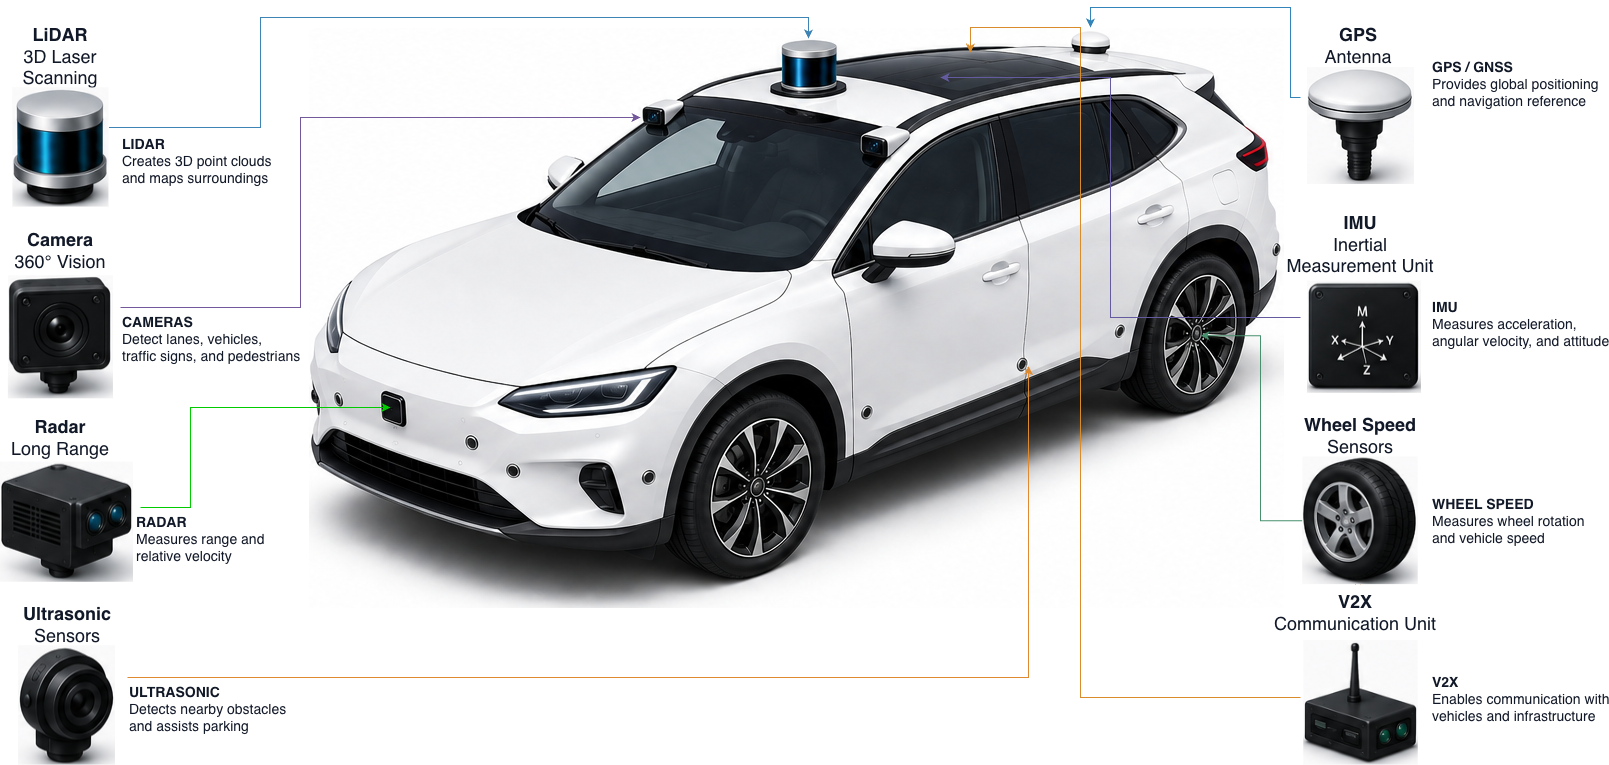
\includegraphics[width=\textwidth]{figures/autonomous_vehicle_sensors_layout_v02.png}
    \caption{Representative autonomous-vehicle sensor layout, showing complementary sensing modalities for perception, localisation, ego-motion estimation, short-range obstacle detection, and communication.}
    \label{fig:autonomous-vehicle-sensors-layout}
\end{figure}

The sensor layout in Fig.~\ref{fig:autonomous-vehicle-sensors-layout} highlights the complementarity that motivates autonomous-driving sensor fusion. The strengths, limitations, and typical fusion roles of the individual modalities are summarised in Tables~\ref{tab:av-onboard-sensors} and~\ref{tab:av-cooperative-inputs}; here we only note the overall pattern: cameras contribute semantics, LiDAR contributes geometry, radar contributes range and velocity under poor visibility, ultrasonic sensors cover the near field, IMUs and wheel odometry provide high-rate ego-motion subject to drift, and GNSS, maps, V2X, and roadside infrastructure extend awareness beyond the onboard field of view.

These modalities are not interchangeable. Instead, each provides a different type of information, with different uncertainty, sampling rate, field of view, latency, and failure modes. Autonomous-driving fusion therefore aims to exploit both \emph{complementarity}, where one sensor provides information that another cannot, and \emph{redundancy}, where multiple sensors observe related aspects of the same scene and can be used for consistency checking, robustness, and fault tolerance.

Table~\ref{tab:av-onboard-sensors} summarises common onboard sensing modalities, while Table~\ref{tab:av-cooperative-inputs} summarises cooperative, localisation, and map-based inputs that support autonomous-driving fusion.

\begin{table}[!t]
    \centering
    \small
    \caption{Onboard sensing modalities commonly used in autonomous-driving sensor fusion.}
    \label{tab:av-onboard-sensors}
    \begin{tabular}{p{0.08\linewidth} p{0.28\linewidth} p{0.30\linewidth} p{0.25\linewidth}}
        \hline
        \textbf{Sensor} & \textbf{Strengths} & \textbf{Limitations} & \textbf{Typical Fusion Role} \\
        \hline
        Camera & Dense appearance, colour, texture, lane markings, traffic signs, traffic lights, and semantic cues & Sensitive to lighting, glare, shadows, night-time conditions, adverse weather, and limited direct depth estimation & Semantic perception, object classification, lane detection, traffic-light recognition, image--LiDAR and image--radar fusion \\
        \hline
        LiDAR & Accurate 3D geometry, depth, object shape, road structure, and point-cloud representation & Higher cost, sparse at long range, affected by rain, fog, snow, and reflective surfaces & 3D object detection, mapping, localisation, free-space estimation, camera--LiDAR fusion \\
        \hline
        Radar & Long range, direct relative velocity, robustness to poor visibility and adverse weather & Lower angular resolution, multipath effects, ghost detections, noisier spatial structure & Object tracking, velocity estimation, long-range detection, radar--camera and radar--LiDAR fusion \\
        \hline
        Ultrasonic & Low-cost short-range sensing, useful for parking and close obstacle detection & Very limited range, low spatial resolution, affected by surface geometry and environmental noise & Low-speed manoeuvring, parking assistance, near-field obstacle detection \\
        \hline
        IMU & High-rate acceleration and angular velocity, useful for short-term ego-motion estimation & Biases and integration drift accumulate over time & Ego-motion prediction, inertial navigation, GNSS--IMU, visual--inertial, and LiDAR--inertial fusion \\
        \hline
        Wheel odometry & Direct vehicle motion information, low cost, high update rate & Accumulates drift, affected by wheel slip, tyre deformation, and road surface conditions & Dead reckoning, vehicle state estimation, GNSS--IMU--odometry fusion \\
        \hline
    \end{tabular}
\end{table}

\begin{table}[!t]
    \centering
    \small
    \caption{Cooperative sensing, localisation, and map-based inputs used in autonomous-driving fusion.}
    \label{tab:av-cooperative-inputs}
    \begin{tabular}{p{0.13\linewidth} p{0.26\linewidth} p{0.28\linewidth} p{0.24\linewidth}}
        \hline
        \textbf{Input} & \textbf{Strengths} & \textbf{Limitations} & \textbf{Typical Fusion Role} \\
        \hline
        GNSS & Provides global positioning in open-sky environments and supports absolute localisation & Degraded by tunnels, urban canyons, multipath, signal blockage, interference, and spoofing risks & Global localisation, correction of accumulated drift in GNSS--IMU, GNSS--wheel odometry, and map-based localisation \\
        \hline
        High-definition maps & Provide prior information about lanes, road boundaries, intersections, landmarks, traffic rules, and road topology & Can become outdated, require accurate localisation, and are costly to build, update, and maintain & Map matching, lane-level localisation, perception priors, planning context, road-structure reasoning \\
        \hline
        V2X communication & Extends perception beyond line of sight and can provide information from nearby vehicles, infrastructure, and traffic-management systems & Depends on connectivity, latency, standardisation, trust, cyber-security, and communication coverage & Cooperative perception, hazard warning, traffic-signal information, occlusion handling, extended situational awareness \\
        \hline
        Roadside infrastructure sensors & Provide external viewpoints from fixed cameras, LiDARs, radars, or smart-city infrastructure & Require deployment and maintenance, depend on communication links, and raise calibration, synchronisation, privacy, and security issues & Infrastructure-assisted perception, validation, cooperative tracking, scenario recording, ground-truth-like reference generation \\
        \hline
    \end{tabular}
\end{table}

\section{Fusion Pipeline and Architectural Levels}

Sensor fusion appears at several points in the autonomous-driving pipeline. A typical system includes sensing, calibration and synchronisation, preprocessing, perception, localisation and mapping, tracking, prediction, planning, and control. Measurements from cameras, LiDAR, radar, ultrasonic sensors, IMUs, wheel encoders, GNSS receivers, maps, V2X messages, and infrastructure sensors must first be temporally synchronised and spatially aligned. This usually requires intrinsic calibration, extrinsic calibration, timestamp correction, latency compensation, motion compensation, and coordinate-frame transformations.

Figure~\ref{fig:autonomous-driving-fusion-pipeline} illustrates the main stages of a typical autonomous-driving sensor-fusion pipeline. The important point is that fusion is not confined to a single block. It can occur repeatedly at different abstraction levels and for different purposes.

\begin{figure}[!t]
    \centering
    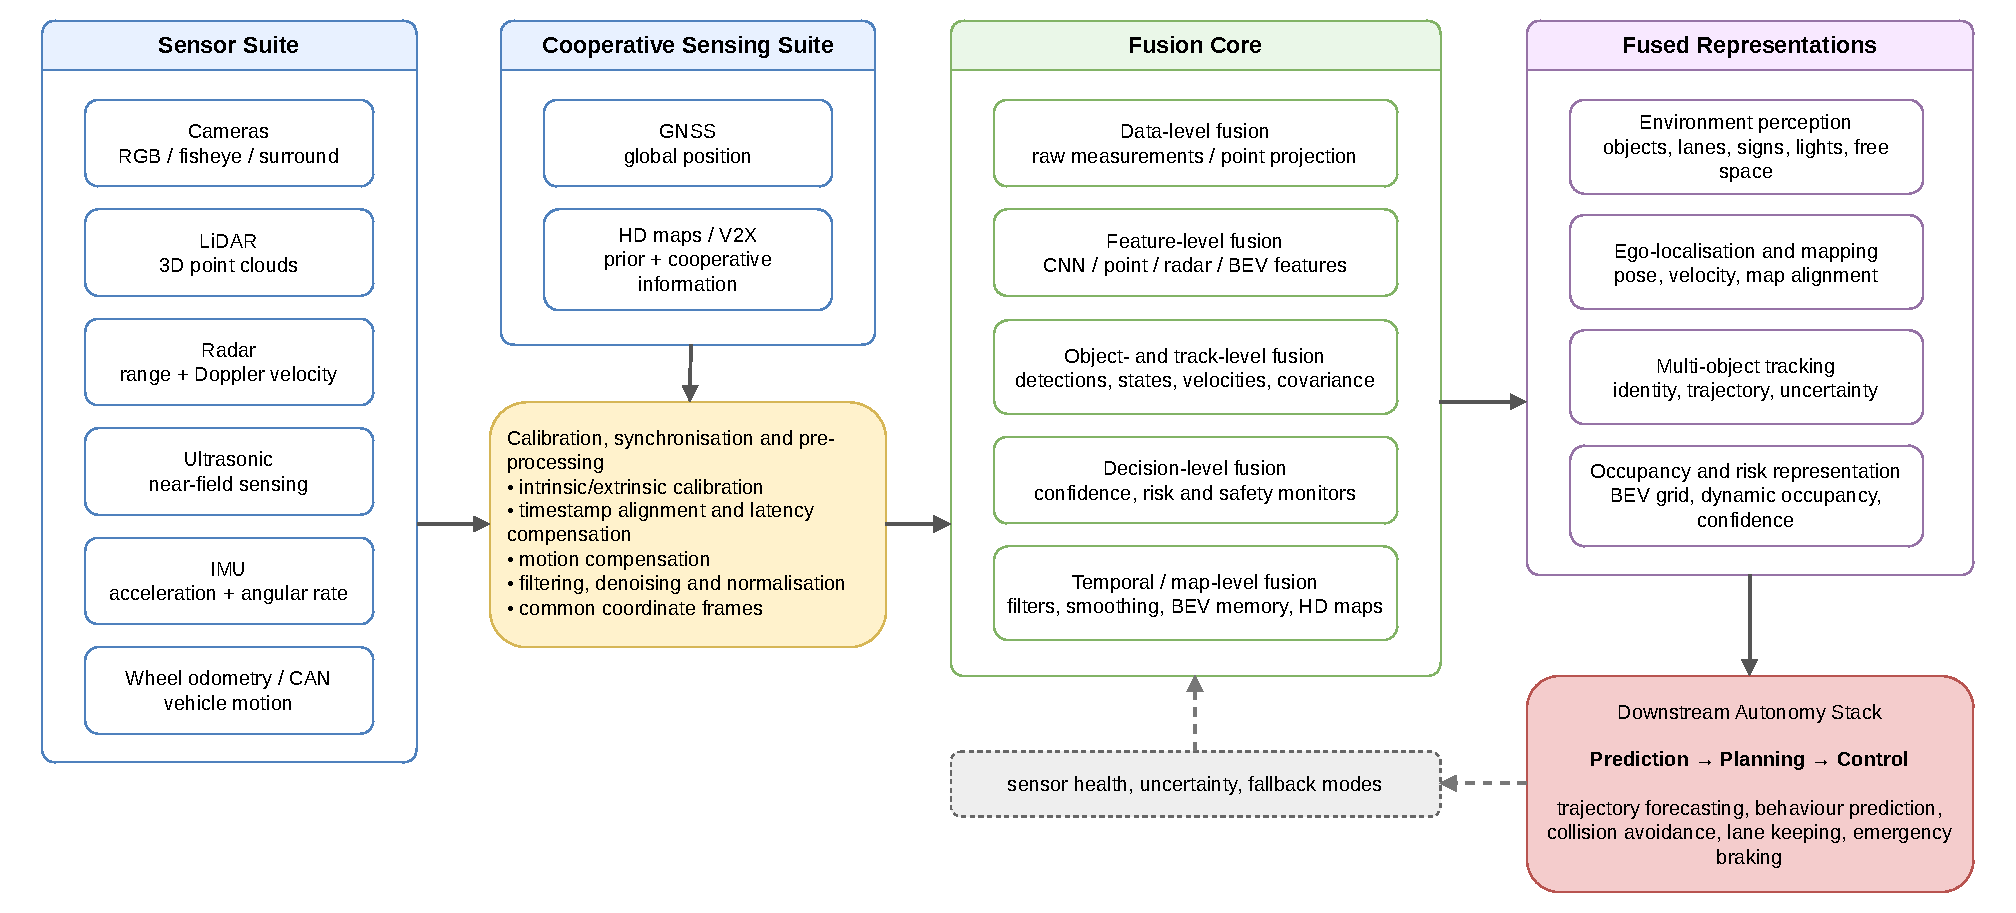
\includegraphics[width=\textwidth]{figures/autonomous_driving_fusion_pipeline.pdf}
    \caption{Autonomous-driving sensor fusion pipeline. Heterogeneous sensor measurements are calibrated, synchronised, and pre-processed before being fused at data, feature, object, decision, temporal, and map levels. The fused representations support environment perception, ego-localisation, mapping, tracking, occupancy estimation, prediction, planning, and control.}
    \label{fig:autonomous-driving-fusion-pipeline}
\end{figure}

Data-level fusion combines low-level measurements directly, for example by projecting LiDAR points into the image plane, aggregating multiple LiDAR sweeps, or associating radar detections with point-cloud clusters. Feature-level fusion combines extracted or learned representations, as in camera--LiDAR, camera--radar, LiDAR--radar, and bird's-eye-view neural architectures. Object- and track-level fusion combines detections, bounding boxes, velocities, class probabilities, covariances, and track states across sensors. Decision-level fusion combines classifier outputs, risk scores, occupancy decisions, or safety-monitoring signals. Temporal fusion uses filtering, smoothing, recurrent networks, temporal attention, or memory-based BEV representations to integrate information over time. Map-level fusion aligns online sensor observations with high-definition maps or previously built local maps.

This layered view clarifies why autonomous driving is a demanding fusion problem. The vehicle must combine onboard exteroceptive sensing for environment perception, proprioceptive sensing for ego-motion estimation, global and map-based references for localisation, and cooperative information for extended situational awareness \cite{2023:IEEE_ITSM,TANG2023109165}. These inputs must then be transformed into representations that are useful for downstream prediction, planning, and control. Errors in calibration, synchronisation, data association, uncertainty modelling, or sensor reliability estimation can therefore propagate through the entire autonomy stack.

\section{Core Fusion Tasks}

Autonomous-driving fusion supports several core tasks. The first is environment perception, where cameras, LiDAR, radar, and maps are used to estimate drivable space, lanes, road boundaries, traffic signs, traffic lights, vehicles, cyclists, pedestrians, and other obstacles. LiDAR depth can improve the spatial accuracy of image-based segmentation, while image semantics can improve the interpretation of sparse point clouds. Radar can contribute long-range range-rate information, especially for moving objects and adverse-weather scenarios. Map priors can further help distinguish valid road areas, pavements, junctions, and lane-level structure.

A second major task is three-dimensional object detection and tracking. Camera--LiDAR fusion is widely used for accurate 3D bounding-box estimation and classification, while radar is valuable for long-range detection and velocity estimation. Tracking extends detection over time by maintaining object identity, position, velocity, acceleration, heading, and uncertainty. Classical filters, smoothing methods, data-association algorithms, and track-management logic remain important even when the detections themselves are produced by deep neural networks.

A third task is ego-localisation and mapping. GNSS, IMU, wheel odometry, cameras, LiDAR, and high-definition maps are fused to estimate the vehicle's position and orientation relative to a local map, global frame, or lane-level map. GNSS alone is insufficient in tunnels, dense urban areas, and multipath environments, while inertial and odometry estimates drift over time. Visual, LiDAR, and map-based localisation can correct this drift, but must handle outdated maps, temporary roadworks, changed lane layouts, perceptual aliasing, and localisation uncertainty.

A fourth task is occupancy, free-space, and risk estimation. Instead of representing the scene only as a list of detected objects, occupancy-based fusion estimates which regions of space are free, occupied, unknown, or dynamically occupied. Risk-aware fusion can incorporate object uncertainty, time-to-collision, occlusion regions, road boundaries, predicted future occupancy, and traffic-rule constraints. These representations are especially important for prediction and planning because the planner must act not only on what is detected, but also on what may be hidden, uncertain, or about to enter the vehicle's path.

Robustness is central to all of these tasks. Rain, fog, snow, darkness, glare, dust, road spray, sensor contamination, and unusual traffic behaviour affect modalities differently. Reliability-aware fusion can adjust sensor weights according to environmental conditions and sensor-health indicators, while temporal fusion can reduce transient false positives and improve consistency. However, fusion cannot compensate for all failures. If several modalities degrade simultaneously, or if the scene lies outside the training or design distribution, the fusion system must detect its own uncertainty and support conservative fallback behaviour.

\section{Datasets, Metrics, and Evaluation}

Public datasets have played a major role in autonomous-driving fusion research. Common benchmarks include KITTI, nuScenes, Waymo Open Dataset, Argoverse, Lyft Level 5, ApolloScape, Oxford RobotCar, Cityscapes, A2D2, ONCE, and BDD100K\addednew{~\cite{geiger2013_kitti,caesar2020_nuscenes,sun2020_waymo,chang2019_argoverse,cordts2016_cityscapes,yu2020_bdd100k}}. These datasets differ in sensor suite, geographic coverage, weather diversity, annotation type, object classes, and supported tasks. A method developed on a camera--LiDAR dataset may not transfer directly to radar fusion, adverse-weather perception, infrastructure-assisted sensing, or map-based localisation. \addednew{Because the datasets named above are dominated by clear-weather scenes, adverse-condition and robustness-oriented benchmarks are increasingly necessary complements: the Seeing Through Fog dataset provides camera--LiDAR--radar recordings in fog, rain, and snow \cite{bijelic2020_stf}, while corruption suites in the style of RoboBEV systematically perturb inputs to probe how BEV fusion architectures degrade \cite{dong2023_robobev}. For a survey whose central claim is robustness through fusion, such benchmarks matter more than average-case leaderboards.} % [July 2026 pass] Dataset name-dropping without citations was a reviewer-visible gap; added citations and an adverse-weather benchmark note. Bib entries in references_additions.bib.

Fusion systems can be evaluated across 2D object detection, 3D object detection, semantic segmentation, panoptic segmentation, lane detection, free-space estimation, multi-object tracking, ego-localisation, odometry, mapping, occupancy prediction, and trajectory prediction. Detection tasks commonly use average precision and mean average precision, while segmentation tasks use intersection-over-union and mean intersection-over-union. Localisation and odometry are often evaluated using absolute trajectory error, relative pose error, drift, heading error, and map-matching accuracy. Tracking metrics additionally assess identity switches, track fragmentation, missed detections, false positives, and trajectory consistency.

For autonomous driving, average benchmark accuracy is not sufficient. Evaluation should also consider latency, throughput, memory footprint, energy consumption, hardware utilisation, uncertainty calibration, false-negative rates for vulnerable road users, robustness under degraded sensing, and performance in rare safety-critical scenarios. Scenario-based testing, simulation, hardware-in-the-loop evaluation, closed-course testing, and real-world trials are important complements to public benchmarks because many critical failures are rare, context-dependent, and difficult to capture in static datasets.

\section{Implementation and Validation}

A practical autonomous-driving fusion system requires more than the fusion algorithm itself. It also requires sensor drivers, calibration tools, data logging, synchronisation mechanisms, coordinate-frame management, visualisation tools, middleware, and deployment-aware software design. ROS and ROS2 are widely used for prototyping because they provide modular communication between sensor, perception, localisation, planning, and control nodes. Python is often used for rapid algorithm development and evaluation, while C++ is commonly used for performance-critical deployment. Deep learning frameworks such as PyTorch and TensorFlow are used for training and evaluating learning-based fusion models.

Practical systems must maintain consistent coordinate frames and timestamps throughout the processing pipeline. This typically requires calibration files, transform trees, time-offset estimation, motion compensation, and careful handling of missing, delayed, or out-of-order messages. Deployment platforms may include CPUs, GPUs, FPGAs, and heterogeneous embedded computing architectures. FPGA-based Kalman and LQG implementations illustrate how estimation cores can be accelerated and validated using hardware-in-the-loop frameworks \cite{deliparaschos_fpgabased_2016}. Such implementations are relevant because latency, energy consumption, and timing determinism become critical when fusion outputs directly affect planning and control.

Several implementation patterns illustrate the connection between fusion theory and deployment. GNSS--IMU--wheel odometry fusion uses inertial and odometry measurements for prediction and GNSS or map-based updates for drift correction. Camera--LiDAR feature-level fusion combines semantic image features with geometric point-cloud or BEV features for 3D perception. Radar--camera--LiDAR track-level fusion associates detections across modalities and maintains object states over time. Reliability-aware fusion adapts sensor weights according to visibility, blockage, timestamp delay, calibration quality, detection confidence, environmental condition, and sensor-health indicators.

System-level validation is essential because real-world fusion performance depends not only on the algorithm, but also on timing, sensor configuration, calibration quality, communication latency, compute resources, and interaction with downstream planning and control. Integrated testing and simulation infrastructures can evaluate sensor fusion components together with perception, control, and human-interaction models \cite{deliparaschos_preliminary_2020}. A concrete example is the Multi-User Environment for Autonomous Vehicle Innovation (MUEAVI), an integrated validation infrastructure for autonomous vehicles and smart-city transport. The facility combines physical road infrastructure, heterogeneous sensor networks, embedded edge processing, a central data-fusion centre, visualisation tools, scenario recording, and software-based validation \cite{deliparaschos_preliminary_2020}.

The MUEAVI camera-tracking pipeline illustrates how infrastructure-level sensing can be connected to perception and actuation through middleware. In this scenario, a full-HD video stream from a PTZ camera is decoded using the NVIDIA DeepStream framework, object detection and tracking are performed, object-detection messages are broadcast through Apache Kafka, and the \texttt{kafka\_ROS\_connector} node converts these messages into custom ROS messages. The \texttt{deepstream\_ptz\_control} node then computes relative pan--tilt--zoom commands from the detected-object list, while the \texttt{ptz\_control} node sends these commands to the PTZ camera and publishes camera status information \cite{deliparaschos_preliminary_2020}. Figure~\ref{fig:mueavi-camera-tracking} illustrates this camera-tracking control-loop validation scenario.

\begin{figure}[!t]
    \centering
    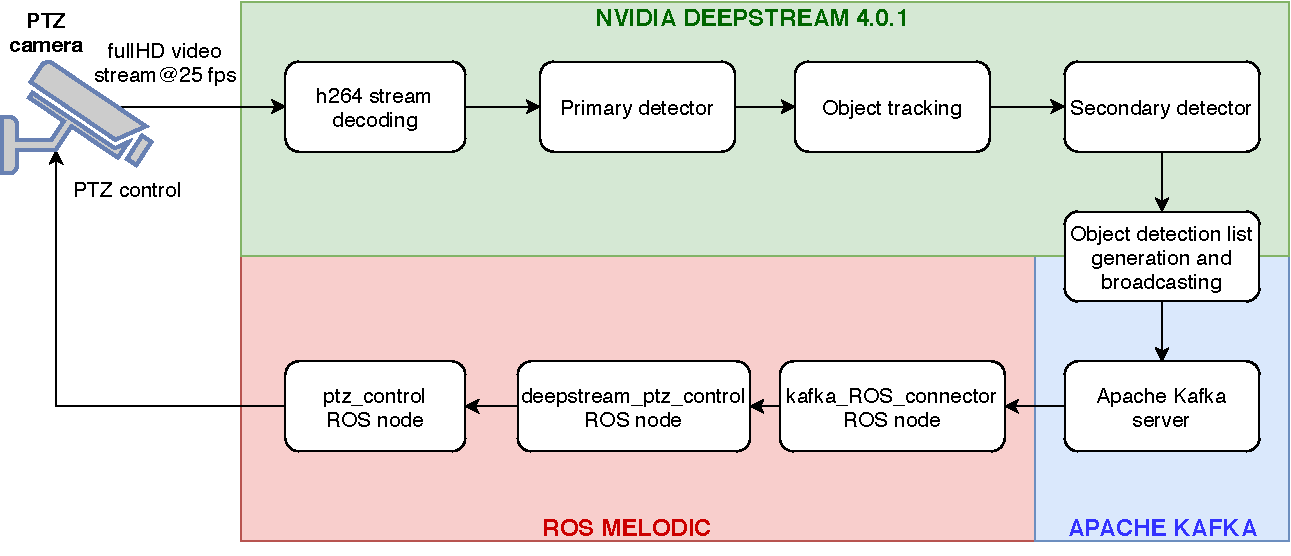
\includegraphics[width=\textwidth]{figures/tracking_with_camera.pdf}
    \caption{Camera tracking control-loop validation scenario based on the MUEAVI infrastructure. The pipeline receives a full-HD video stream from a PTZ camera, decodes it using the NVIDIA DeepStream framework, performs object detection and tracking, broadcasts object-detection messages through Apache Kafka, and converts these messages into ROS messages using the \texttt{kafka\_ROS\_connector} node. The \texttt{deepstream\_ptz\_control} ROS node computes relative pan--tilt--zoom commands from the detected-object list, while the \texttt{ptz\_control} ROS node sends the commands to the PTZ camera and publishes camera status information.}
    \label{fig:mueavi-camera-tracking}
\end{figure}

Infrastructure-supported fusion systems extend this idea by combining data from vehicle-mounted and fixed sensing sources. Roadside cameras, LiDARs, and radars can observe vehicles and vulnerable road users from viewpoints that differ from those available to the ego vehicle. This can improve object tracking, support cooperative perception, provide external validation for onboard perception, and help analyse occluded or safety-critical scenarios.

A representative infrastructure-assisted architecture consists of three layers. The first layer performs local acquisition and preprocessing close to the sensors, including video decoding, timestamping, point-cloud filtering, radar parsing, clustering, and object detection. Camera-based detection can be implemented using real-time neural detectors such as YOLOv3 \cite{redmon_yolov3_2018}. LiDAR and radar preprocessing commonly involves point-cloud filtering, downsampling, segmentation, and clustering, with tools such as the Point Cloud Library and algorithms such as DBSCAN being widely used in practical implementations \cite{rusu_pcl_2011, ester_dbscan_1996}. The second layer performs centralised or distributed fusion, including coordinate transformation, multi-object tracking, object classification, sensor-selection logic, and scenario classification. The third layer supports validation, visualisation, data storage, and comparison against simulation or reference measurements.

This type of architecture connects sensor fusion with verification and validation rather than treating it as an isolated perception module. It also exposes practical implementation issues that are often hidden in algorithm-only descriptions, including time synchronisation, multi-sensor cross-calibration, middleware design, network latency, edge-computing constraints, and real-time data storage. Hardware--software co-design and systematic sensor-selection methods are therefore relevant when fusion algorithms must be deployed on embedded or resource-constrained platforms \cite{deliparaschos_fpga_2016}.

% ============================================
\chapter{Sensor Fusion in Multi-Agent Systems}
\label{sec:MAS}
% ============================================
\deleted{[Needs to be expanded, needs references, perhaps a numerical example]} % Addressed: graph-theoretic setting and consensus references added below, together with a worked numerical example.
Multi-agent sensor fusion extends the single-platform view by allowing several vehicles, robots, infrastructure nodes, or monitoring stations to share information about a common environment. The fused state may describe the pose of each agent, the state of external objects, a shared map, a risk field, or the health of a distributed infrastructure. This setting is increasingly important in autonomous driving, aerial robotics, smart-city monitoring, maritime surveillance, and critical-infrastructure protection, where a single agent may be occluded, communication-limited, or unable to observe the whole scene.

The main benefit of multi-agent fusion is complementary viewpoint diversity. In cooperative driving, for example, a roadside camera or another connected vehicle may observe a pedestrian hidden behind a parked truck from the ego vehicle's perspective. In aerial robotics, several drones can jointly localise themselves and map an environment while individual GNSS, vision, or range measurements are intermittent. In maritime monitoring, AIS, coastal radar, satellite imagery, and cable-based sensing form a distributed observation network rather than a single colocated sensor suite. These examples show that multi-agent fusion is not merely more data; it changes the observability, latency, trust, and coordination structure of the estimation problem.

Architecturally, multi-agent fusion can be centralised, decentralised, or hybrid. In a centralised architecture, agents transmit measurements, features, tracks, or local maps to a fusion centre, which performs association, estimation, and decision-making. This can produce a globally consistent estimate, but it requires communication bandwidth, low enough latency, and a trusted computational node. In a decentralised architecture, each agent maintains its own estimate and exchanges selected information with neighbours. Consensus filters, distributed Kalman filters, distributed particle filters, covariance-intersection methods, and belief-function frameworks are representative tools when no single node has all information or when cross-correlations are unknown \cite{khaleghi_multisensor_2013,foglietta_networked_2012}.

\deleted{[Too short this stuff about consensus. What is a neighbor? a graph? needs some explanation and reference if we want to use it.]}
\addednew{The natural abstraction for decentralised fusion is a communication graph $\mathcal{G}=(\mathcal{V},\mathcal{E})$, where the node set $\mathcal{V}=\{1,\dots,N\}$ collects the agents and an edge $(i,j)\in\mathcal{E}$ indicates that agents $i$ and $j$ can exchange information directly, for example over a V2V or V2I link. The \emph{neighbour set} $\mathcal{N}_i=\{j:(i,j)\in\mathcal{E}\}$ of agent $i$ therefore contains exactly the agents it can hear at a given time; no agent needs global knowledge of the network. Classical results show that if the graph is connected (or, for time-varying and directed networks, suitably jointly connected), simple local averaging rules drive all agents to agreement, with convergence speed governed by the algebraic connectivity of the graph \cite{olfatisaber2007_consensus,ren2005_consensus}.}
{\color{blue}
The simplest decentralised mechanism is the consensus filter, in which each agent $i$ repeatedly averages its local estimate with those of its communication neighbours,
\begin{equation}
\widehat{\mathbf{x}}_i(k+1)=\widehat{\mathbf{x}}_i(k)+\epsilon\sum_{j\in\mathcal{N}_i}\left(\widehat{\mathbf{x}}_j(k)-\widehat{\mathbf{x}}_i(k)\right),
\label{eq:consensus-filter}
\end{equation}
where $\mathcal{N}_i$ is the neighbour set of agent $i$ and $\epsilon>0$ is a step size bounded by the inverse of the maximum node degree. Under mild connectivity assumptions, all local estimates converge to a common value, so a network can agree on a fused state using only local exchanges. In practice, consensus iterations are interleaved with local measurement updates (consensus-on-information or consensus-on-measurement filters), and when the cross-correlations between agents' estimates are unknown, the covariance-intersection rule of \eqref{eq:ci-cov}--\eqref{eq:ci-est} in Section~\ref{subsec:track-fusion} provides the consistent way to merge the exchanged estimates.
}

{\color{RevisionOlive}
\begin{example}
Consider four vehicles on a path graph $1$--$2$--$3$--$4$ (each vehicle communicates only with its immediate neighbours), holding local range estimates to a common obstacle of $\widehat{x}_1(0)=10$, $\widehat{x}_2(0)=12$, $\widehat{x}_3(0)=11$, and $\widehat{x}_4(0)=15$ metres. The maximum node degree is $2$, so any step size $\epsilon<1/2$ is admissible; take $\epsilon=0.3$. One application of \eqref{eq:consensus-filter} yields
\begin{equation*}
\widehat{x}_1(1)=10.6,\,
\widehat{x}_2(1)=11.1,\,
\widehat{x}_3(1)=12.5,\,
\widehat{x}_4(1)=13.8.
\end{equation*}
Note that the sum (and hence the average, $12$) is preserved at every iteration; continued iterations contract the spread geometrically, and all four estimates converge to the network average $12$~m without any vehicle ever communicating beyond its neighbours. The outlier estimate of vehicle~4 is thus absorbed gradually, which also illustrates the main operational caveats: consensus requires several communication rounds per fused value, and a faulty or malicious agent biases the entire network unless it is detected and discounted.
\end{example}
}

Hybrid architectures are often the most practical: local edge nodes perform fast preprocessing and tracking, while a regional or cloud-level node performs slower map update, validation, learning, or fleet-level coordination \cite{deng_edge_2021,lim_federated_2020}.

The information exchanged between agents strongly affects both performance and deployability. Raw-data sharing can preserve the most information but is expensive and sensitive to synchronisation, calibration, and privacy constraints. Feature-level sharing reduces bandwidth and can support learned cooperative perception, but it requires compatible representations and careful uncertainty calibration. Object- or track-level sharing is efficient and interpretable, but it depends on reliable local detection, association, and covariance or confidence estimates. Decision-level sharing is the lightest option and is useful for warnings, alerts, or manoeuvre coordination, but it may hide the uncertainty and conflict that generated the decision. The choice of communication level is therefore a fusion-design decision, not only a networking detail.

Multi-agent fusion also introduces failure modes that are less visible in single-agent systems. Communication delays can make received information stale; packet losses can create intermittent measurements; inconsistent coordinate frames can corrupt cooperative tracks; duplicated information can cause overconfident estimates; and compromised or faulty agents can inject misleading evidence. Conservative fusion methods, including covariance intersection, evidence-theoretic conflict measures, innovation monitoring, and set-membership consistency checks, are therefore valuable when cross-agent dependencies or trust levels are uncertain. In connected automated vehicles, set-membership methods have been used to support shared situational awareness under occlusion, while evidence-distance and Dempster--Shafer approaches have been applied to real-time inter-vehicle data fusion \cite{narri2021_set_membership_shared_awareness,cho_realtime_2020}.

Validation is particularly demanding because the relevant scenarios involve both sensing and communication. A convincing evaluation should vary not only weather, occlusion, object density, and sensor degradation, but also network latency, packet loss, agent density, viewpoint overlap, calibration error, clock offset, malicious data, and inconsistent local maps. For safety-critical deployment, multi-agent fusion should expose the provenance of fused information, the age of received data, the assumed trust in each source, and the remaining uncertainty after cooperation. The open research challenge is to obtain the robustness benefits of cooperation without allowing communication constraints, correlation errors, or untrusted agents to make the fused estimate less reliable than a well-designed local estimate.

% ============================================
\chapter{Applications Beyond Autonomous Vehicles}
\label{sec:applications}
% ============================================
\deleted{[This paragraph doesn't make much sense and anyway not here. Seems a leftover]} % Resolved: the leftover was replaced by the bridging paragraph below (blue).
\added{The two case studies in this section are deliberately chosen to show how \emph{all} the classical ingredients of Chapter~\ref{sec:classicalSF} --- Kalman filtering and innovation monitoring, evidence-theoretic conflict handling, and MCDM-based prioritisation --- combine into complete fusion systems in a domain far from autonomous driving. They should be read as integrative worked examples of the survey's toolbox rather than as an exhaustive treatment of maritime sensing.}

\section{Maritime Anomaly Detection and Infrastructure Protection}

Maritime anomaly detection is a representative application in which sensor fusion is needed because no single information source provides a complete and trustworthy maritime picture. The Automatic Identification System (AIS) provides vessel identity, position, speed, course, and other navigation information, but AIS messages can be missing, delayed, spoofed, or intentionally misleading. Coastal radar, electro-optical and infrared cameras, satellite imagery, synthetic-aperture radar, hydrophones, and distributed acoustic sensing can provide independent observations, but each modality has different coverage, resolution, latency, and false-alarm characteristics. Recent surveys of AIS anomaly detection highlight the diversity of abnormal behaviours that must be considered, including route deviation, loitering, unexpected stops, speed anomalies, encounter anomalies, and suspicious gaps in transmission \cite{wolsing_anomaly_2022}. This problem is becoming more relevant as maritime navigation systems become increasingly digital and interconnected, exposing the fused navigation pipeline itself to faults, spoofing, and cyber--physical disturbances \cite{oliva_innovation_2026}.

The practical difficulty is that suspicious behaviour is not always dramatic. A vessel may keep transmitting AIS in order to avoid immediate suspicion while still performing small route deviations, abnormal speed profiles, unusual loitering, or manoeuvres close to protected infrastructure. This is especially relevant in congested and geopolitically sensitive regions such as the Baltic Sea, where normal maritime traffic coexists with dense networks of submarine power and communication cables. A maritime fusion architecture should therefore combine trajectory analysis with contextual information: proximity to coastlines, shipping lanes, restricted areas, cable corridors, anchorages, recent incidents, weather, and vessel class.

At the trajectory level, fusion typically starts by constructing vessel tracks from AIS and radar measurements, associating visual or satellite detections with those tracks, and extracting behavioural features such as speed over ground, course change, distance from shipping lanes, proximity to restricted areas, encounter geometry, and consistency between reported identity and observed motion. Remote-sensing imagery and AIS can also be fused to identify small vessels or vessels whose reported AIS state is inconsistent with the observed scene \cite{chen_sviadf_2025}. Graph-based route models provide an additional layer of context: a recent Baltic Sea framework constructs a Probabilistic Roadmap (PRM) of feasible maritime corridors, projects AIS trajectories onto this graph, and derives interpretable features such as route inefficiency, deviation from learned corridors, and speed or dwell time near submarine cables \cite{oliva_tomei_prm_access_2026}. This illustrates a broader design principle: raw trajectories become more informative when fused with geospatial constraints and infrastructure maps.

Maritime anomaly detection should also include the estimation layer. In navigation and monitoring systems, GNSS, inertial sensors, radar, and AIS may be fused through Kalman-filter-based estimators. Some cyber--physical anomalies or stealthy disturbances may first appear as abnormal innovations before they become visible as large trajectory deviations. Innovation-based monitoring can therefore test whether the residual sequence remains zero-mean, covariance-consistent, Gaussian, and temporally white; such diagnostics can expose coloured spoofing or disturbance patterns that may bypass a simple \(\chi^2\) covariance check \cite{oliva_innovation_2026}. This connects ship anomaly detection directly to the sensor-fusion pipeline rather than treating it only as offline post-processing of AIS tracks.

Evidence theory is well suited to this setting because maritime anomalies are often ambiguous. A vessel moving slowly near a cable route may be fishing, drifting because of a mechanical problem, performing maintenance, or preparing an illegal anchoring activity. A frame of discernment can include hypotheses such as \emph{normal transit}, \emph{loitering}, \emph{route deviation}, \emph{AIS inconsistency}, \emph{collision risk}, \emph{infrastructure threat}, and \emph{unknown}. AIS-derived behaviour, radar tracks, camera detections, satellite observations, innovation-test alarms, and acoustic or cable-sensing cues can each provide BBAs over this frame. If several sources support the same abnormal hypothesis, the fused belief increases. If AIS reports normal transit while radar, imagery, or cable sensing indicates inconsistent behaviour, the conflict mass becomes an operator-relevant warning rather than being hidden inside a single confidence score.

MCDM can complement this process by ranking alerts and response actions. Criteria may include distance to protected infrastructure, confidence of track association, deviation from learned maritime corridors, innovation-test alarms, severity of the suspected anomaly, persistence over time, weather and visibility, vessel type, traffic density, and expected operator workload. AHP-style pairwise comparisons can encode expert preferences from coast guards, port authorities, or infrastructure operators, while real-time sensor indicators provide the criterion scores. The resulting MCDM score can prioritise which anomalies require immediate attention, which sensors should be tasked for confirmation, or which vessels should be monitored more closely.

The main challenges are data quality, class imbalance, interpretability, and validation. True anomalous events are rare and often poorly labelled, while normal maritime traffic varies strongly with geography, season, weather, and port operations. Synthetic anomalies, incident-based case studies, and infrastructure-aware features can help evaluate candidate methods, but broader external validation remains necessary \cite{oliva_tomei_prm_access_2026}. For operational deployment, a transparent combination of track-level fusion, innovation monitoring, evidence-theoretic uncertainty handling, and MCDM-based prioritisation can be more useful than a black-box anomaly score alone.

\section{Sensor Fusion for Submarine Cable Monitoring}

Submarine power and telecommunication cables are critical infrastructures for digital connectivity, energy interconnection, offshore wind farms, and security-sensitive maritime operations \cite{carter_submarine_2009,kavanagh_achieving_2025}. They are exposed to accidental and intentional hazards such as anchor dragging, bottom trawling, seabed instability, fatigue, construction activity, and deliberate tampering. Anchor-related events are particularly important, with the risk depending on anchor geometry, burial depth, seabed properties, and vessel drift \cite{yoon_safety_2013,osthoff_anchor_soil_2017,li_anchor_risk_2025}. Monitoring is difficult because the relevant events are spatially distributed, the assets extend over tens or hundreds of kilometres, and damaging interactions may be masked by waves, currents, seabed coupling, and ordinary vessel activity.

Distributed acoustic sensing (DAS) turns an optical fibre into a dense array of strain or strain-rate measurements by interrogating backscattered light along the cable \cite{hartog_intro_2017,lu_distributed_2019,lindsey_fiberoptic_2021}. In marine environments, this is attractive because seafloor instrumentation is difficult and expensive to deploy, while existing or dedicated fibre-optic cables may cover long distances with metre-scale spatial sampling. Long-term subsea deployments show that DAS can support real-time detection of bottom-trawl fishing, ship anchoring, and seismic events over cable spans of operational length \cite{waagaard_longterm_2022}, and related demonstrations cover seismic, hydroacoustic, and power-cable strain sensing \cite{williams_distributed_2019,matsumoto_hydroacoustic_2021,masoudi_dynamic_2018}.

For underwater-cable monitoring, DAS can support several fusion tasks. First, it can provide spatially distributed acoustic or deformation evidence of nearby vessels, anchors, trawling activity, sediment motion, or cable vibration. Second, it can be fused with AIS, radar, bathymetry, weather, ocean-current estimates, and maintenance records to interpret the cause of the observed signal. Third, it can support infrastructure protection by detecting events close to telecom cables, power cables, pipelines, offshore wind farms, or port approaches. Experimental work using an optical telecom cable offshore Toulon showed that ship-radiated noise could be detected and, in favourable conditions, used for trajectory estimation \cite{rivet_ship_2021}, while more recent Applied Ocean Research work studies DAS-based vessel monitoring using submarine fibre-optic cables in the presence of growing offshore infrastructure and vessel traffic \cite{paap_vessel_2025}. For power cables, \(\phi\)-OTDR experiments have also been used to distinguish calm sea, anchor drop, and anchor drag signatures \cite{lv_otdr_2018}.

The fusion problem is challenging because DAS measurements are not equivalent to conventional hydrophone measurements. The response depends on cable coupling to the seabed, cable orientation relative to the incoming wavefield, gauge length, interrogation settings, local bathymetry, and the propagation path. Some cable segments may be well coupled to the seafloor, while suspended or poorly coupled sections may respond differently. A robust fusion system should therefore include a cable-state model and should not treat all DAS channels as equally reliable.

Model-based monitoring can help bridge the gap between raw distributed measurements and actionable alarms. Cable dynamics can be approximated through physically grounded tensioned-structure models, with finite-dimensional state-space approximations providing a natural interface to filtering and diagnosis \cite{irvine_linear_1974,baudouin_cable_pde_2018}. 

In a recent paper~\cite{fioravanti_cable_med_2026} this direction is followed by modelling a submarine cable as a damped tensioned structure, obtaining a finite-dimensional state-space approximation, and applying Kalman filtering to distributed deformation measurements. Under nominal conditions, the filter innovations should remain statistically consistent with the model and the assumed environmental excitation. Localised mechanical interactions, such as an anchor strike or tampering event, appear as systematic deviations in the innovation sequence and can be detected using sliding-window statistical tests. This approach complements purely data-driven DAS processing because it introduces physical interpretability and separates stochastic environmental forcing from persistent structural perturbations.

Evidence theory can be used to represent uncertainty in event interpretation. For a cable segment and time window, the hypotheses may include \emph{passing vessel}, \emph{anchoring or trawling risk}, \emph{seismic event}, \emph{oceanographic background}, \emph{cable-coupling artefact}, \emph{mechanical tampering}, and \emph{unknown}. DAS spectral features, distributed deformation residuals, AIS proximity, radar tracks, hydrophone data, bathymetry, and environmental models can each assign belief masses. High conflict, such as a strong cable disturbance without a nearby AIS vessel, may indicate an unreported vessel, missing data, a non-vessel geophysical source, or a localised mechanical interaction requiring inspection.

MCDM is useful for prioritising alerts and sensor resources. Criteria may include signal-to-noise ratio, distance to the cable, estimated vessel size, consistency with AIS, innovation-test significance, persistence of the event, cable criticality, environmental conditions, and cost of dispatching inspection assets. The same framework can rank candidate explanations or decide whether to request additional confirmation from patrol vessels, satellite imagery, or nearby fixed sensors. In this way, DAS-based cable monitoring becomes a full sensor-fusion problem: dense acoustic or deformation sensing provides the raw evidence, physical models and filters structure the residuals, and contextual maritime data and decision logic turn that evidence into actionable situation awareness.

\chapter{Open Challenges and Future Directions}
\label{sec:open-challenges}

\section{Robustness Under Adverse and Long-Tail Conditions}

Sensor-fusion systems must operate under rare, degraded, and difficult-to-model conditions. In autonomous driving, these include adverse weather, unusual lighting, rare road users, roadworks, emergency vehicles, sensor blockage, and unusual traffic behaviour. In other domains, such as maritime monitoring or critical-infrastructure protection, long-tail events may include spoofed reports, missing data, rare vessel behaviours, or infrequent physical disturbances. Public datasets only partially cover such cases, while synthetic augmentation may not fully reproduce real sensor degradation. Future work should develop more realistic sensor-corruption models, richer adverse-condition datasets\addednew{~\cite{bijelic2020_stf,dong2023_robobev}}, and evaluation protocols that reward robust behaviour rather than only average-case performance.

\section{Calibration Drift, Sensor Failure, and Degraded Modalities}

Fusion performance depends strongly on calibration, synchronisation, and sensor health. Mechanical vibration, temperature change, sensor replacement, clock drift, communication delays, or physical obstruction can introduce spatial or temporal misalignment. Sensors may also be blocked, degraded, spoofed, saturated, or damaged. Future systems require online calibration monitoring, automatic fault detection, sensor-health estimation, and fusion architectures that degrade gracefully when one or more modalities become unreliable.

\section{Uncertainty Estimation, Conflict Handling, and Explainability}

Many learning-based fusion systems produce accurate predictions but poorly calibrated confidence estimates. For safety-critical applications, the system must know when it does not know. Future research should improve uncertainty estimation, out-of-distribution detection, explainable sensor weighting, and conflict detection between modalities. Hybrid approaches that combine neural perception with probabilistic estimation, evidence theory, fuzzy logic, or interpretable reliability models are promising because they can expose why a sensor was trusted, down-weighted, or treated as conflicting.

\section{Real-Time Embedded Deployment}

Modern fusion architectures can be computationally expensive, especially when they use high-resolution images, dense point clouds, radar tensors, distributed acoustic measurements, temporal histories, or transformer-based attention. Real-time deployment requires careful optimisation of latency, memory, power consumption, communication bandwidth, and hardware utilisation, on automotive-grade platforms such as NVIDIA DRIVE Orin, Qualcomm Snapdragon Ride, TI TDA4-class SoCs, and FPGA-based accelerators\deleted{ [Cite something?]}\addednew{~\cite{lin2018_architectural,liu2019_edge_computing,sze2017_efficient}}. Future research should consider efficient model design, sparse computation, quantisation, hardware-aware training, and co-design between algorithms and embedded platforms.

\section{Verification, Validation, and Safety Assurance}

Sensor-fusion systems must be validated under a very large scenario space, including rare events, sensor failures, degraded sensing, and conflicting inputs. Simulation, scenario-based testing, closed-course testing, hardware-in-the-loop systems, real-world trials, and formal safety arguments are all required. A key open problem is how to validate learning-based fusion systems whose behaviour depends on high-dimensional data and may not be easily interpretable. Validation should therefore assess not only task accuracy, but also uncertainty calibration, fault tolerance, graceful degradation, and the effect of fusion errors on downstream decisions. \addednew{Emerging automotive standards give this challenge a concrete regulatory shape: ISO~26262 addresses functional safety of electronic systems, ISO~21448 (SOTIF) addresses hazards arising from functional insufficiencies of the intended behaviour --- including perception and fusion errors without any hardware fault --- and ISO/PAS~8800 targets safety of AI-based functions in road vehicles. A fusion architecture whose uncertainty, conflict, and degradation signals are explicit, as advocated throughout this survey, is substantially easier to argue about under these frameworks than an end-to-end black box.} % [July 2026 pass] A V&V subsection in a 2026 automotive survey should acknowledge the applicable safety standards; added without new bib entries (standards are cited by designation, as is common in IEEE Access).

{\color{blue}
\section{Sim-to-Real Transfer and Continual Adaptation}

\deleted{[I don't completely follow. this paragraph is short and could be more informative.]} % Addressed in the previous round: subsection rewritten (blue block).

Learning-based fusion models are increasingly trained or augmented in simulation, because rare and dangerous scenarios are cheap to generate synthetically. However, simulated sensor models rarely reproduce the detailed failure characteristics of real cameras, LiDAR, and radar --- noise textures, multipath, blooming, spray, or weather-dependent attenuation --- so models can inherit a sim-to-real gap precisely in the degraded conditions for which simulation was used. Closing this gap requires physically faithful sensor simulation, domain-adaptation techniques evaluated per modality, and validation protocols that measure transfer explicitly. A related challenge is continual and online learning: fusion systems that adapt during deployment (recalibrating reliability weights, updating maps, or fine-tuning detectors) must do so without catastrophic forgetting and without invalidating prior safety arguments.

\section{Privacy, Standardisation, and Interoperability}
\deleted{[I don't completely follow. this paragraph is short and could be more informative.]} % Addressed in the previous round: subsection rewritten (blue block).
Multi-agent and infrastructure-assisted fusion make data governance a first-order design constraint. Cooperative perception exchanges observations of identifiable people and vehicles across organisational boundaries, raising privacy, retention, and consent questions that pure onboard fusion avoids; techniques such as feature-level sharing, anonymisation, and federated learning trade information content against privacy exposure. Interoperability is equally unresolved: V2X message formats, coordinate conventions, time bases, uncertainty representations, and trust models must be standardised before fused estimates from heterogeneous vendors can be combined safely. Without agreed ways to exchange covariances, confidences, and provenance, receiving agents cannot apply the consistency mechanisms (covariance intersection, evidence discounting) that this survey has argued are essential.
}

\section{Foundation Models and End-to-End Fusion}
\deleted{[I don't completely follow. this paragraph is short and could be more informative.]}
Recent progress in large-scale representation learning and foundation models may influence future sensor-fusion systems. Large multimodal models could improve generalisation, semantic reasoning, and data efficiency, while end-to-end architectures may learn integrated perception, prediction, planning, or monitoring representations. However, these approaches raise important questions about interpretability, safety, uncertainty, data bias, compute requirements, and failure analysis. Future fusion research must determine how to combine the flexibility of large learned models with the reliability, structure, and auditability required for safety-critical operation.

\addednew{Two concrete developments illustrate the trend. First, planning-oriented end-to-end architectures such as UniAD train perception, prediction, and planning jointly in a single network, so that fusion is no longer an explicit module but an emergent property of intermediate representations \cite{hu2023_uniad}; recent surveys of end-to-end driving systematise the rapidly growing design space and its open problems, including causal confusion, covariate shift, and the difficulty of interpreting intermediate features \cite{chen2024_e2e_survey}. Second, large multimodal language models are being explored as high-level reasoning layers on top of fused perception, for instance to interpret rare scenes, explain decisions in natural language, or serve as a semantic prior for long-tail objects \cite{cui2024_mllm_driving}. For the fusion perspective taken in this survey, the key open questions are where the classical safety layer should sit when the fusion function is implicit --- for example, whether innovation-style consistency checks can be applied to latent representations --- how calibrated uncertainty can be extracted from end-to-end models, and whether foundation-model outputs can be treated as one more (highly capable but occasionally unreliable) information source to be discounted and audited with the conflict-handling machinery of Chapter~\ref{sec:classicalSF}.}

% ============================================
\chapter{Concluding Remarks}
\label{sec:conclusions}
% ============================================

This book has presented a tutorial and survey of sensor fusion for autonomous driving vehicles. By focusing on autonomous driving as the central application domain, the book has connected classical fusion methods, learning-based multimodal perception, reliability-aware reasoning, practical implementation, and safety-critical evaluation. Classical methods such as Bayesian filtering, statistical fusion, evidence theory, and optimisation remain essential for localisation, tracking, uncertainty management, and sensor-health reasoning. Learning-based methods, particularly deep multimodal and bird's-eye-view fusion, have become central to perception tasks such as object detection, segmentation, tracking, and occupancy estimation.

Set-membership and zonotopic estimation add a conservative bounded-error layer for consistency checking, complementing probabilistic and learning-based fusion when explicit guarantees are needed.

A central theme of this survey is that robust autonomous driving requires more than combining sensor outputs for improved benchmark accuracy. Fusion systems must also handle calibration errors, asynchronous data, adverse weather, sensor degradation, out-of-distribution scenes, computational constraints, and uncertainty propagation. The interaction between fusion outputs and downstream prediction, planning, and control means that safety, latency, interpretability, and fault tolerance must be considered throughout the design process.

\deleted{[Check what follows.]} % Checked and approved.
\added{If a single lesson is to be drawn from this survey, it is that additional sensors improve a system only when their measurement models, uncertainties, and mutual dependencies are represented honestly: an ignored correlation, a miscalibrated covariance, or an unmodelled failure mode can make a fused estimate confidently wrong, which is worse than being uncertain. The corollary is architectural: learned perception and classical estimation are not competitors but layers, with the classical layer supplying the uncertainty bookkeeping that makes learned outputs safe to act on.}

Future research is likely to move towards hybrid architectures that combine the representational power of deep learning with the structure, uncertainty handling, and interpretability of classical estimation and decision-making methods. Progress will also depend on improved datasets, more realistic robustness benchmarks, efficient embedded deployment, and rigorous verification and validation. Sensor fusion will therefore remain a core research and engineering challenge in the development of safe, reliable, and scalable autonomous driving vehicles. \deleted{[This is chatgpt 100\%. but the idea of a final personal address is nice.]}\added{We hope this survey serves as both a map and an invitation: the most valuable near-term contributions are likely to come not from a single better detector or filter, but from the disciplined integration of the two traditions reviewed here, and from the community adopting shared benchmarks that reward calibrated uncertainty and graceful degradation rather than average-case accuracy alone.}

\chapter*{Acknowledgements}
\addcontentsline{toc}{chapter}{Acknowledgements}
\addednew{The authors thank the anonymous reviewers for their constructive comments, which substantially improved the structure and completeness of this survey.} % [July 2026 pass] Placeholder acknowledgement text retained from the original source.

\backmatter
\bibliographystyle{unsrt}
\bibliography{references}

% ============================================
% About the Authors
% ============================================
\chapter*{About the Authors}
\addcontentsline{toc}{chapter}{About the Authors}

\begin{authorbiography}[{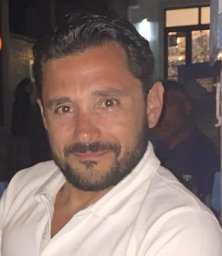
\includegraphics[width=1in,height=1.25in,clip,keepaspectratio]{figures/kdeliparaschos.jpg}}]{Kyriakos M. Deliparaschos} (Senior Member, IEEE) received his B.Eng. (Hons) in Electronic Engineering and M.Sc. in Mechatronics from De Montfort University, UK, and the National Technical University of Athens (NTUA), Greece. He earned his Ph.D. from the Department of Signals, Control and Robotics, School of Electrical and Computer Engineering, NTUA, Greece. He currently holds a Special Teaching Staff position in the Department of Electrical Engineering, and Computer Science and Engineering (EECSE) at the Cyprus University of Technology (CUT), Cyprus. He has held academic and research positions at New York College and IST College in Athens, Greece; NTUA, Greece; CUT, Cyprus; Trinity College Dublin, Ireland; and Cranfield University, UK. His research interests include embedded systems, reconfigurable hardware acceleration, sensor fusion, resilient cyber-physical systems, intelligent control, real-time robotic navigation, and medical robotics for minimally invasive surgery.
\end{authorbiography}


\begin{authorbiography}[{
\includegraphics[width=1in,height=1.25in,clip,keepaspectratio]{figures/goliva.jpg}}]{Gabriele Oliva} (Senior Member, IEEE) received the M.Sc and the Ph.D. degrees in computer science and automation engineering from the University Roma Tre of Rome, Italy, in 2008 and 2012, respectively. He is currently an Associate Professor in automatic control with the University Campus Bio-Medico of Rome, Italy, where he directs the Complex Systems \& Security Laboratory\deleted{.} (CoserityLab). Since 2022, he is an Associate Editor for the IEEE Control Systems Letters Journal. Moreover, he has been an Associate Editor for the Conference Editorial Board of the IEEE Control Systems Society and for PLOS ONE. His main research interests include distributed multi-agent systems, optimisation, decision-making, maritime situation awareness, and critical infrastructure protection.
\end{authorbiography}

\begin{authorbiography}[{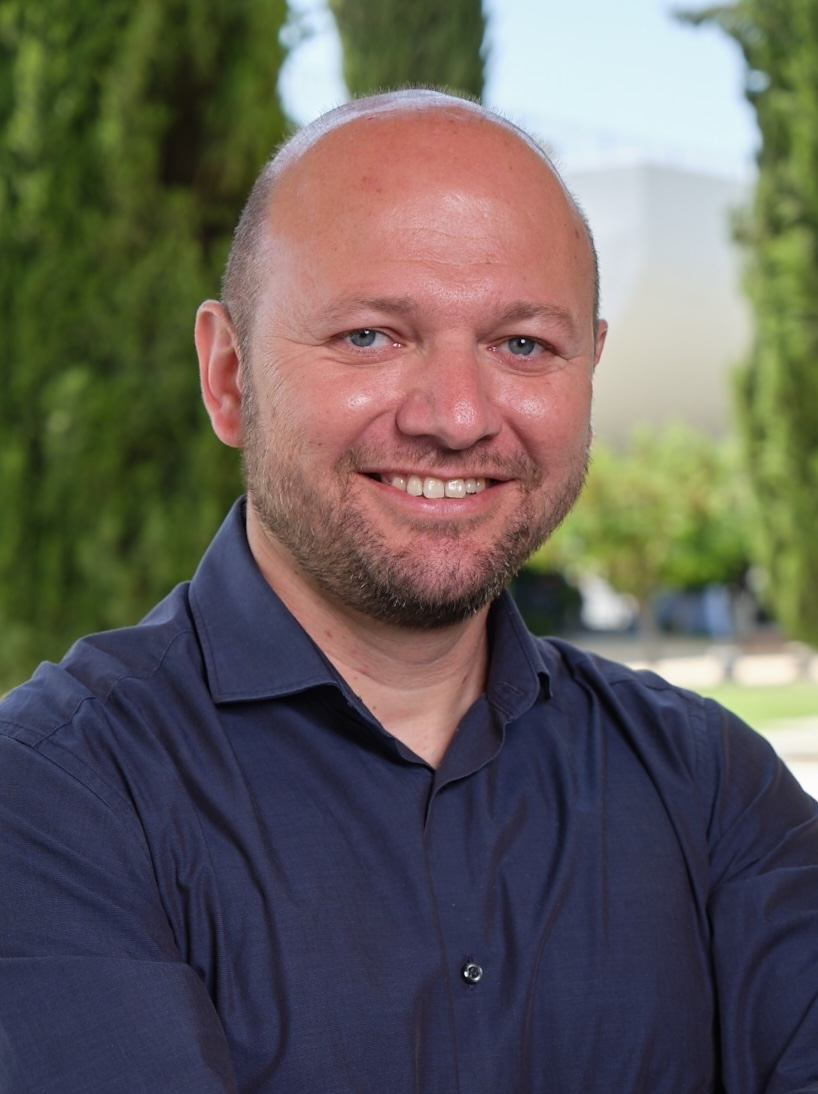
\includegraphics[width=1in,height=1.25in,clip,keepaspectratio]{figures/themis4-papers.jpg}}]{Themistoklis Charalambous}~(Senior Member, IEEE) received the BA (First Class
Honours) and M.Eng. (Distinction) degrees in Electrical and Information Sciences from Trinity College, University of Cambridge, and the Ph.D. degree from the Control Laboratory, Department of Engineering, University of Cambridge.
%
Following his PhD, he held research and teaching positions at
Imperial College London, the University of Cyprus, KTH Royal Institute of Technology, and Chalmers University of Technology.
%
In 2017, he joined the Department of Electrical Engineering and Automation, School of Electrical Engineering, Aalto University, as an Assistant Professor; he was awarded the
title of Academy Research Fellow by the Academy of Finland in 2018 and was promoted to Associate Professor in 2020.
%
In September 2021, he joined the Department of Electrical and Computer Engineering, University of Cyprus, as a tenure-track Assistant Professor.
\added{In May 2022, he received an ERC Consolidator Grant for the project ``MINERVA: Emerging Cooperative Autonomous Systems: Information for Control and Estimation.''}
Since May 2026, he has been a tenured Associate Professor at the University of Cyprus. He is also a Visiting Professor at Aalto University and, since April 2023, at the FinEst Centre for Smart Cities.
%In September 2021, he continued his academic career at the University of Cyprus, where he joined the Department of Electrical and Computer Engineering as a tenure-track Assistant Professor. In May 2022, he was awarded an European Research Council (ERC) Consolidator Grant for the research project “MINERVA: Emerging Cooperative Autonomous Systems: Information for Control and Estimation.” From May 2026, he was appointed as a tenured Associate Professor at the University of Cyprus. He also remains affiliated with Aalto University as a Visiting Professor and, since April 2023, serves as a Visiting Professor at the FinEst Centre for Smart Cities.
%
%Prof. Charalambous is an Associate Editor of \textsc{IEEE Transactions on Automatic Control}
\end{authorbiography}

% ============================================
% End of book
% ============================================
\end{document}
